\chapter{Future Near Detectors for Long Baseline Neutrino Oscillation Experiments}\label{sec:hptpc}

For T2K, the statistical error is still the largest uncertainty on oscillation measurements. This will not be the case for the future long baseline neutrino oscillation experiments, HK and DUNE, and so they aim to perform 5$\sigma$ measurements of $\delta_{CP}$. However, as the statistical error becomes less significant, it is ever more important that systematic uncertainties are reduced. To achieve the target sensitivity, systematic errors will need to be reduced to the 1-2$\%$ level.

As discussed in Section \ref{sec:eb}, cross-section uncertainties are the dominant systematic, and these depend heavily on theoretical nuclear models. This is because the target nucleon resides inside a nucleus, and so nuclear effects and final state interactions (FSI) alter the measured kinematics of final state particles. As discussed in Section \ref{sec:interactions}, FSI effects cause the neutrino energy to be reconstructed incorrectly, and interactions to be misclassified, contributing a large systematic uncertainty. To reduce these uncertainties, tensions in nuclear models must be resolved, which can only be done with improved measurements of the multiplicity and momentum distributions of final state particles \cite{nustecscat}.

The NEUT, GENIE, and NuWro \cite{nuwro} neutrino event generators use cascade models tuned to hadron-nucleus scattering measurements to simulate final-state particles leaving the target nucleus. However, these measurements are sparse, as shown in Figure \ref{fig:nucxsec}, and so semi-empirical parametrisations are used to extrapolate to the relevant momentum ranges and target nuclei. The parametrisations are different in the three generators, leading to significant differences in the multiplicity of final state protons, as shown in Figure \ref{fig:generators}. Below 100 MeV, the proton momentum distributions diverge considerably, but this is below the detection threshold of current detectors.

\begin{figure}
\centering
\includegraphics*[width=0.75\textwidth,clip]{figs/nucxsec}
\caption{Cross-section measurements of protons on different nuclei. Figure from \cite{hptpcprop}.}\label{fig:nucxsec}
\end{figure}

\begin{figure}
\centering
\includegraphics*[width=0.8\textwidth,clip]{figs/neutgenienuwro}
\caption{Predicted proton energy distributions at the DUNE far detector using GENIE, NEUT and NuWro. The dashed and solid lines show the expected reconstruction thresholds in liquid and 10 atm gaseous argon detectors respecctively. Figure from \cite{dunehptpc}.}\label{fig:generators}
\end{figure}

It is therefore crucial that future near detectors are able to accurately measure final state particles, particularly at low momentum, to distinguish between nuclear models and reduce the effects of FSI.

\section{High Pressure Time Projection Chamber}

A high pressure time projection chamber (HPTPC) is a proposed near detector for future long baseline neutrino oscillation experiments. It is designed to be able to probe the low momentum region of parameter space to resolve nuclear model tensions and reduce neutrino interaction cross-section uncertainties.

Gas TPCs have lower momentum thresholds for detecting secondary particles as low energy hadrons travel further from the interaction point in gas than in denser detectors. The proton detection threshold is $\sim$110 MeV in water Cerenkov detectors, and $\sim$400 MeV in liquid argon TPCs. These are both too high to resolve model discrepancies. 

The main disadvantage of using gas as an active target is the reduction in number of events due to the lower density, but this effect can be reduced by increasing the pressure. This, combined with the Mega-Watt beams future experiments will utilise, mean there can be enough detected events using a gaseous target.

Having the TPC filled with the active target allows 4-$\pi$ angular coverage of final state particles, further adding to the HPTPC's ability to distinguish between interaction models.

An HPTPC is part of the planned near detector complex at DUNE, and T2K has explored the possibility of using an HPTPC as a long term near detector upgrade. 

\subsection{Single Transverse Variables}

When the true momentum vector of the final state lepton and hadrons are projected into the plane transverse to the original neutrino’s trajectory, any momentum imbalance is due to final state interactions and nuclear effects. By making accurate measurements of the multiplicity and momentum distributions of secondary particles, an HPTPC can probe the missing momentum, and better characterise events affected by FSI. This can be done using single transverse kinematics variables (STV) \cite{stv1}:

\begin{itemize}

\item $\delta p_{T}$: represents the imbalance in the three momentum in the transverse plane. It is zero in the absence of FSI.

\item $\delta \phi_{T}$: characterises how `back-to-back' the transverse components in the final states are. It is zero for a completely balanced final state.

\item $\delta \alpha_{T}$: describes how the hadronic system has been `accelerated' or `decelerated' by FSI effects. This is $<\pi$/2 if the proton transverse momentum is larger than expected for the observed lepton transverse momentum, and $>\pi$/2 if the proton transverse momentum is smaller than expected.

\end{itemize}

The geometric definitions of these variables in the plane transverse to the neutrino direction are shown in Figure \ref{fig:stvdef}.

\begin{figure}
\centering
\includegraphics*[width=0.8\textwidth,clip]{figs/HorizSTV}
\caption{Definition of the single transverse variables in the plane transverse to the neutrino direction. Figure from \cite{stv2}.}\label{fig:stvdef}
\end{figure}

These kinematics are also less dependent on the true incoming neutrino energy, which is not precisely known for individual events in accelerator neutrino experiments. Using these transverse variables can therefore provide insight into final state interactions and nuclear effects \cite{stv3}.

\subsection{Sensitivity Studies}

HPTPC simulation was produced to explore the potential sensitivity improvement from using an HPTPC. This was done by smearing the true kinematics of a subset of ND280 FGD1 MC events. For each event, for both the momentum and angle of the final state lepton, a random number was drawn from a Gaussian with mean equal to the true value of the variable in the ND280 MC, and width equal to the assumed resolution of the HPTPC. The assumed resolutions are shown in Table \ref{tab:hptpcres}.

The selection of events is similar to that described in Section \ref{sec:sel}, but using the full FGD1 volume. The assumed detection thresholds were different for the ND280 and HPTPC selections, as shown in Table \ref{tab:hptpcthresh}. The thresholds are the only differences between the ND280 and HPTPC MC.

The selected events are then divided by pion and proton multiplicity, giving seven samples in total:

\begin{center}
\begin{table}[!htbp]
\center
\begin{tabular}{l l||c}
\hline \hline
\multicolumn{2}{c||}{\textbf{Value}} & \textbf{Fractional Resolution}\\
\hline
\hline
$p_{\mu}$ & $<200$ MeV & 0.036 \\
 & 200-400 MeV & 0.043 \\
 & 400-600 MeV & 0.053 \\
 & 600-800 MeV & 0.070 \\
 & 800-1000 MeV & 0.090 \\
 & 1000-1200 MeV & 0.093 \\
 & 1200-1400 MeV & 0.110 \\
 & 1400-1600 MeV & 0.120 \\
 & 1600-1800 MeV & 0.125 \\
 & $>1800$ MeV & 0.130 \\  
\hline
cos$\theta_{\mu}$ & $<1$, $>-1$ & 0.040 \\
\hline \hline
\end{tabular}
\caption{Assumed HPTPC $p_{\mu}$ and cos$\theta_{\mu}$ resolutions.}
\label{tab:hptpcres}
\end{table}
\end{center}

\begin{center}
\begin{table}[!htpb]
\center
\begin{tabular}{c ||c c}
\hline \hline
 & \multicolumn{2}{c}{\textbf{Detection Threshold (MeV)}}\\
\textbf{Particle} & \textbf{ND280} & \textbf{HPTPC} \\
 \hline \hline
$\mu^{\pm}$ & 100 & 15 \\
$\pi^{\pm}$ & 120 & 16 \\
$p$ & 450 & 60 \\
\hline \hline
\end{tabular}
\caption{Assumed detection thresholds used in these studies for the HPTPC and ND280 MC.}
\label{tab:hptpcthresh}
\end{table}
\end{center}

\vspace{-1cm}
\begin{itemize}

\item \textbf{CC 0$\pi$ 0p:} 1 muon above threshold, 0 charged pions above threshold, 0 protons above threshold.

\item \textbf{CC 0$\pi$ 1p:} 1 muon above threshold, 0 charged pions above threshold, 1 proton above threshold.

\item \textbf{CC 0$\pi$ Np:} 1 muon above threshold, 0 charged pions above threshold, $>1$ protons above threshold.

\item \textbf{CC 1$\pi$ 1p:} 1 muon above threshold, 1 charged pion above threshold, 0 protons above threshold.

\item \textbf{CC 1$\pi$ 1p:} 1 muon above threshold, 1 charged pion above threshold, 1 proton above threshold.

\item \textbf{CC 1$\pi$ Np:} 1 muon above threshold, 1 charged pion above threshold, $>1$ protons above threshold.

\item \textbf{CC Other:} 1 muon above threshold, $>1$ charged pions above threshold.

\end{itemize}

The cross-section and flux systematics from the 2015 T2K oscillation analysis, described in \cite{tn265} and \cite{tn217} respectively, were applied. The main difference to the interaction model described in Section \ref{sec:xsec} is that a Relativistic Fermi Gas (RFG), rather than Spectral Function (SF), nuclear model was used. The flux model was tuned using data from a thinner replica target experiment than the model described in Section \ref{sec:flux}. Detector systematics have not been developed for the HPTPC, so weren't applied to either the HPTPC or ND280 MC.

The total number of events in each sample, for each detector, are shown in Table \ref{tab:hptpcrates}.

\begin{center}
\begin{table}[!htbp]
\center
\begin{tabular}{l ||c c}
\hline \hline
& \multicolumn{2}{c}{\textbf{Events}}\\
\textbf{Sample} & \textbf{ND280} & \textbf{HPTPC} \\
 \hline \hline
CC 0$\pi$ 0p & 3165.52 & 645.38 \\
CC 0$\pi$ 1p & 3038.75 & 4956.65 \\
CC 0$\pi$ Np & 491.36 & 2634.29 \\
CC 1$\pi$ 0p & 1296.50 & 833.26 \\
CC 1$\pi$ 1p & 1094.97 & 1719.41\\
CC 1$\pi$ Np & 94.69 & 516.67 \\
CC Other & 1104.51 & 1348.12 \\
\hline
Total & 10286.30 & 12653.78 \\
\hline \hline
\end{tabular}
\caption{Number of events in each sample for the ND280 and HPTPC MC.}
\label{tab:hptpcrates}
\end{table}
\end{center}

The CC 0$\pi$ 0p and CC 1$\pi$ 0p samples have more events for ND280, as higher multiplicity events will be misclassified as having zero protons due to the higher detection thresholds. Overall, there is a greater number of interactions in the HPTPC sample, due to the lower thresholds.

The $p_{\mu}$-cos$\theta_{\mu}$ distributions for the two detectors are shown in Figures \ref{fig:nd280PmuTmu} and \ref{fig:hptpcPmuTmu}.

\begin{figure}
\centering
\begin{subfigure}{.49\textwidth}
  \centering
  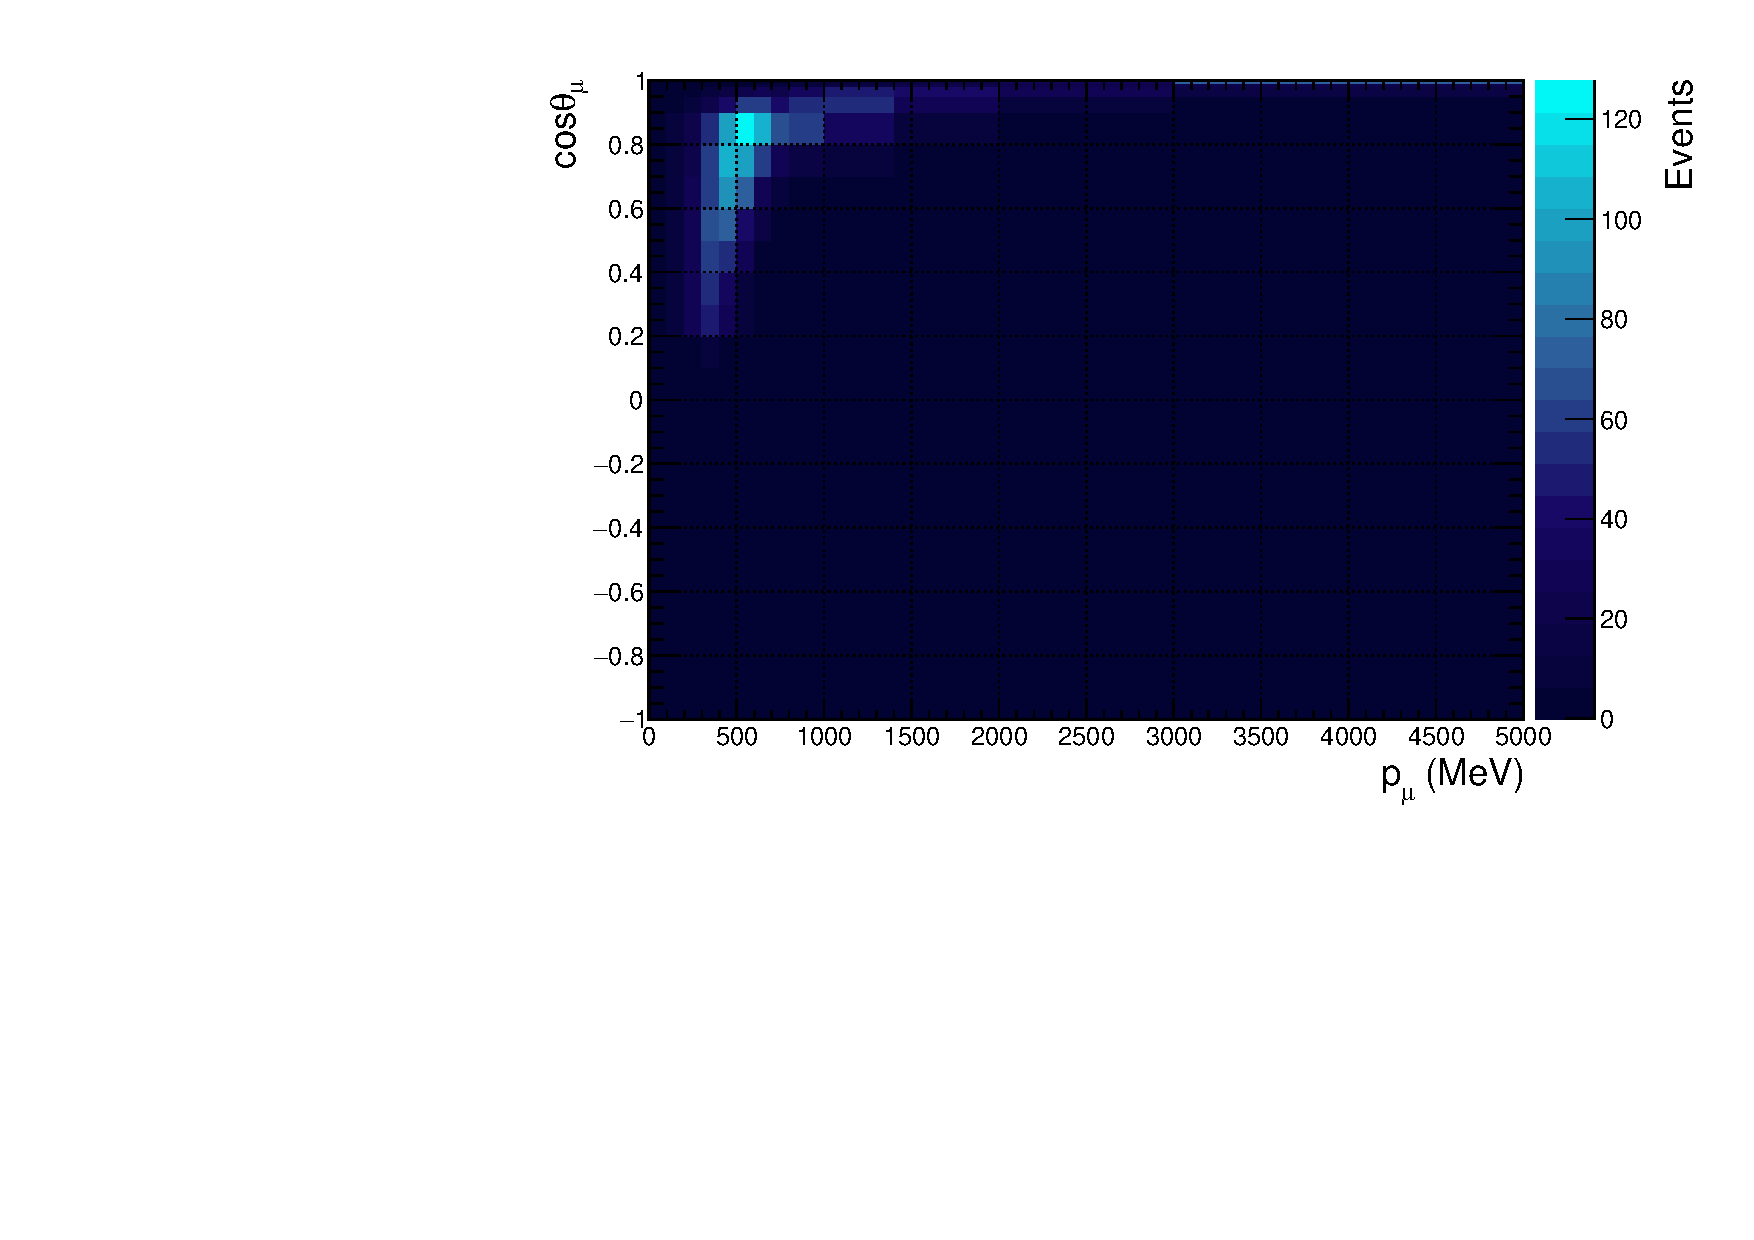
\includegraphics[width=0.9\linewidth]{figs/nd280_pmtmuu_cc0pi0p.pdf}
  \caption{CC 0$\pi$ 0p}
\end{subfigure}
\begin{subfigure}{.49\textwidth}
  \centering
  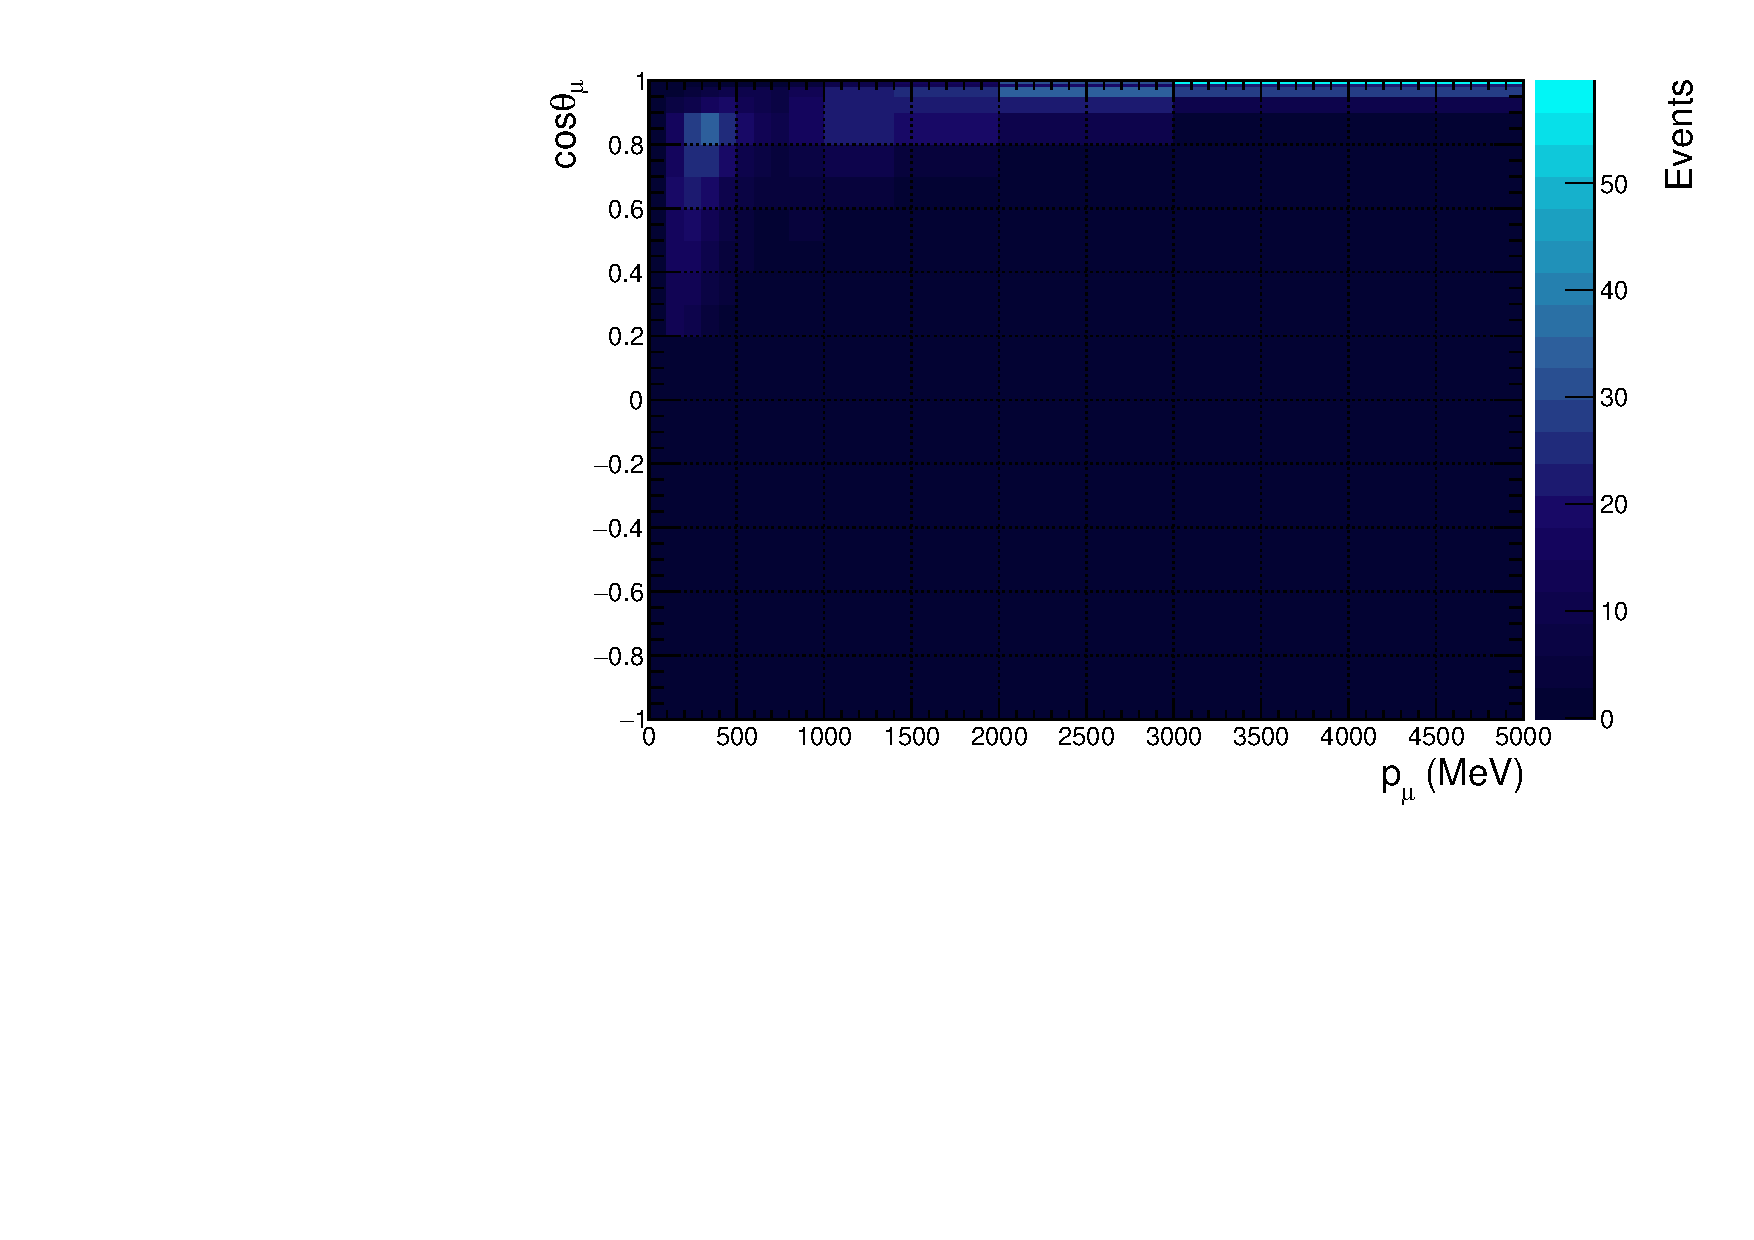
\includegraphics[width=0.9\linewidth]{figs/nd280_pmtmuu_cc1pi0p.pdf}
  \caption{CC 1$\pi$ 0p}
\end{subfigure}
\begin{subfigure}{.49\textwidth}
  \centering
  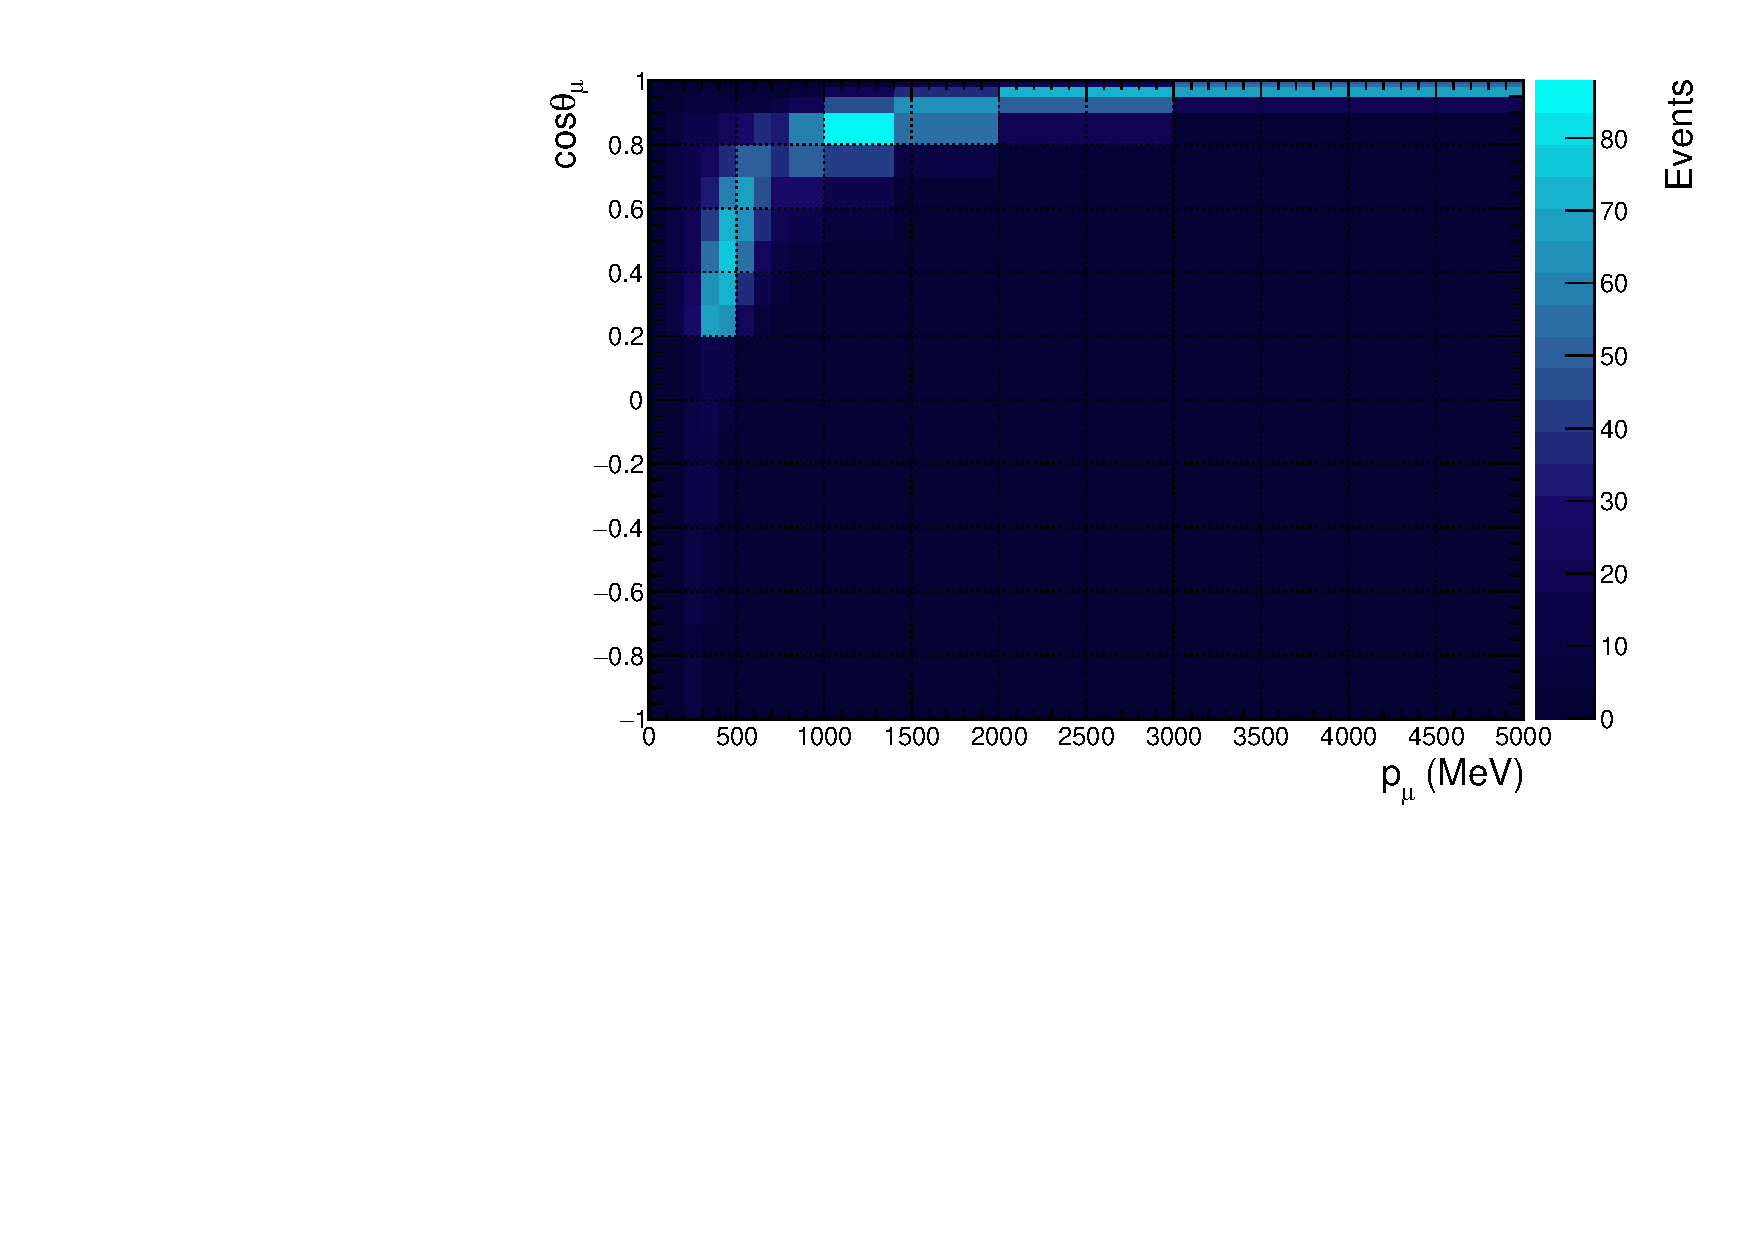
\includegraphics[width=0.9\linewidth]{figs/nd280_pmtmuu_cc0pi1p.pdf}
  \caption{CC 0$\pi$ 1p}
\end{subfigure}
\begin{subfigure}{.49\textwidth}
  \centering
  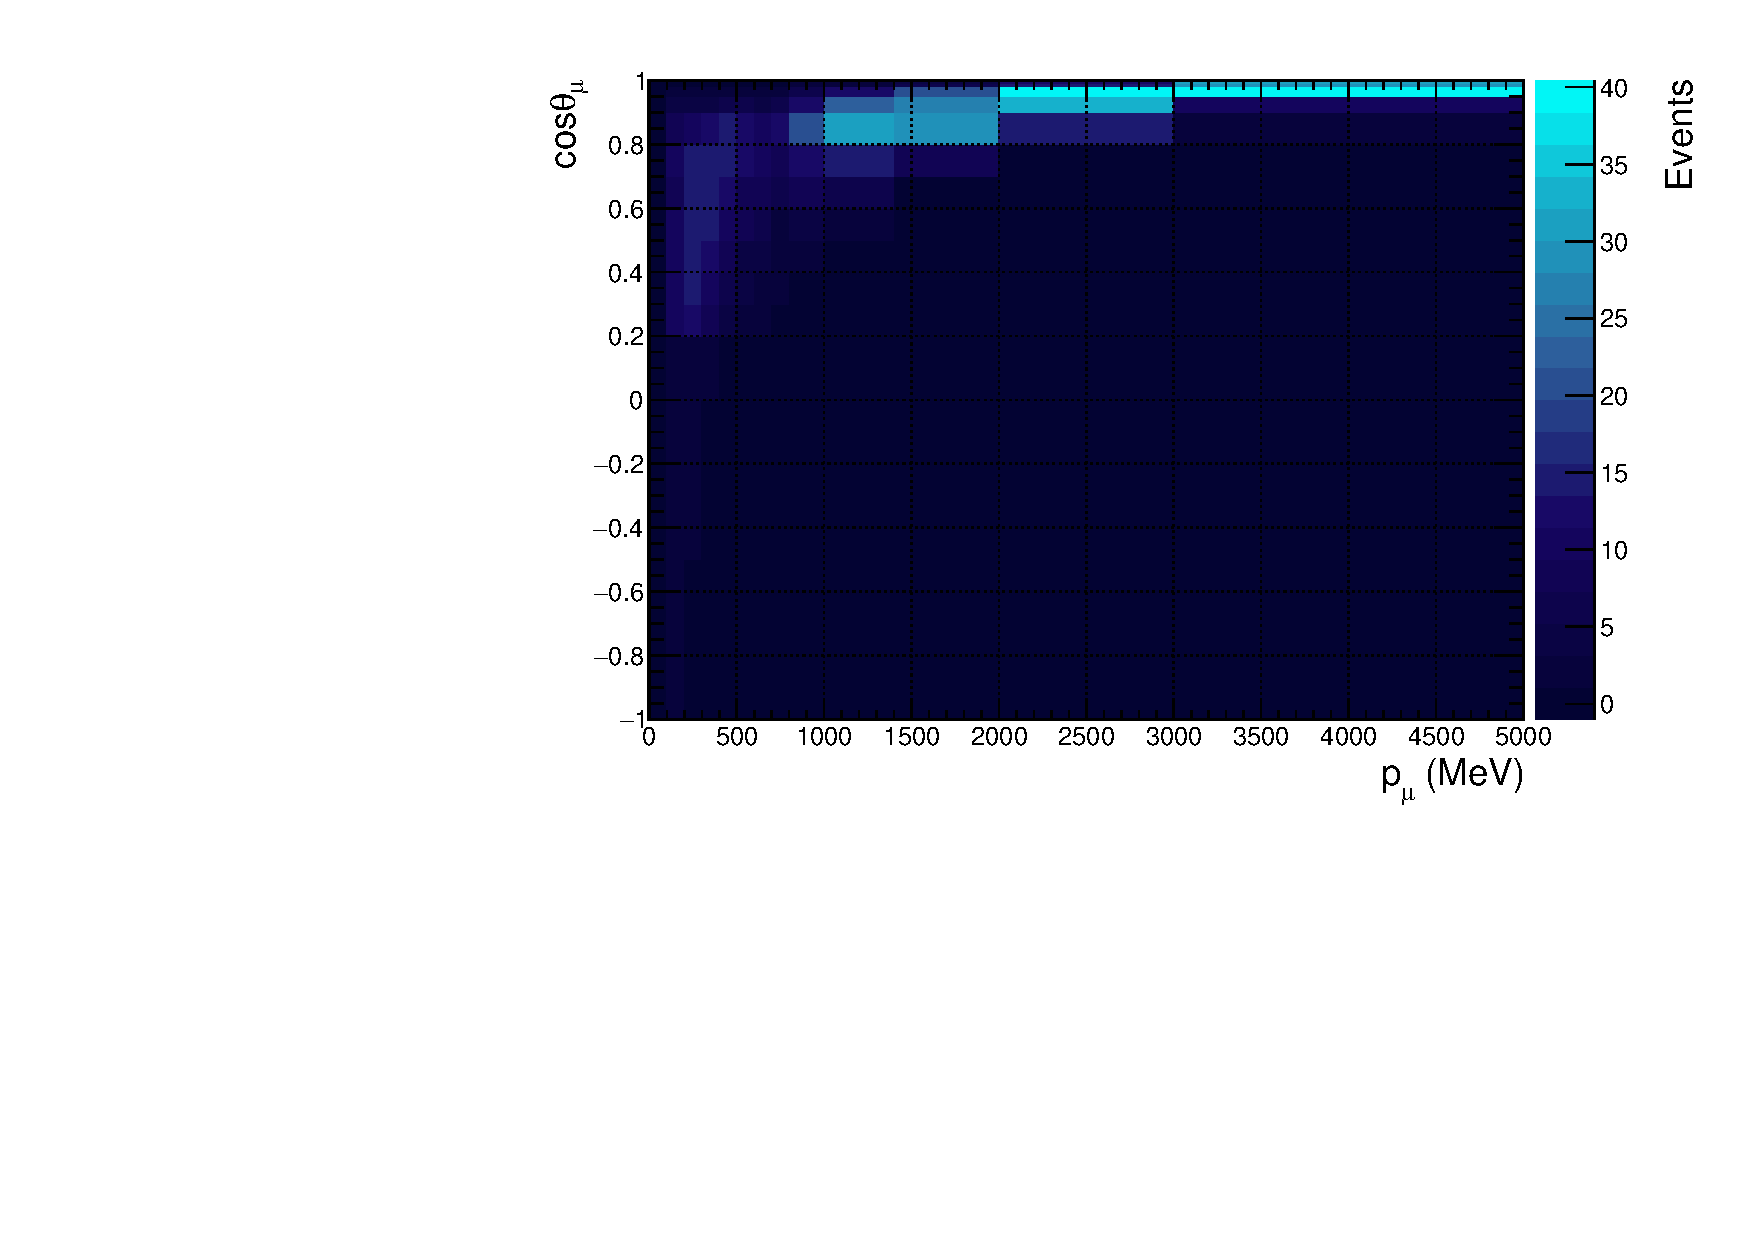
\includegraphics[width=0.9\linewidth]{figs/nd280_pmtmuu_cc1pi1p.pdf}
  \caption{CC 1$\pi$ 1p}
\end{subfigure}
\begin{subfigure}{.49\textwidth}
  \centering
  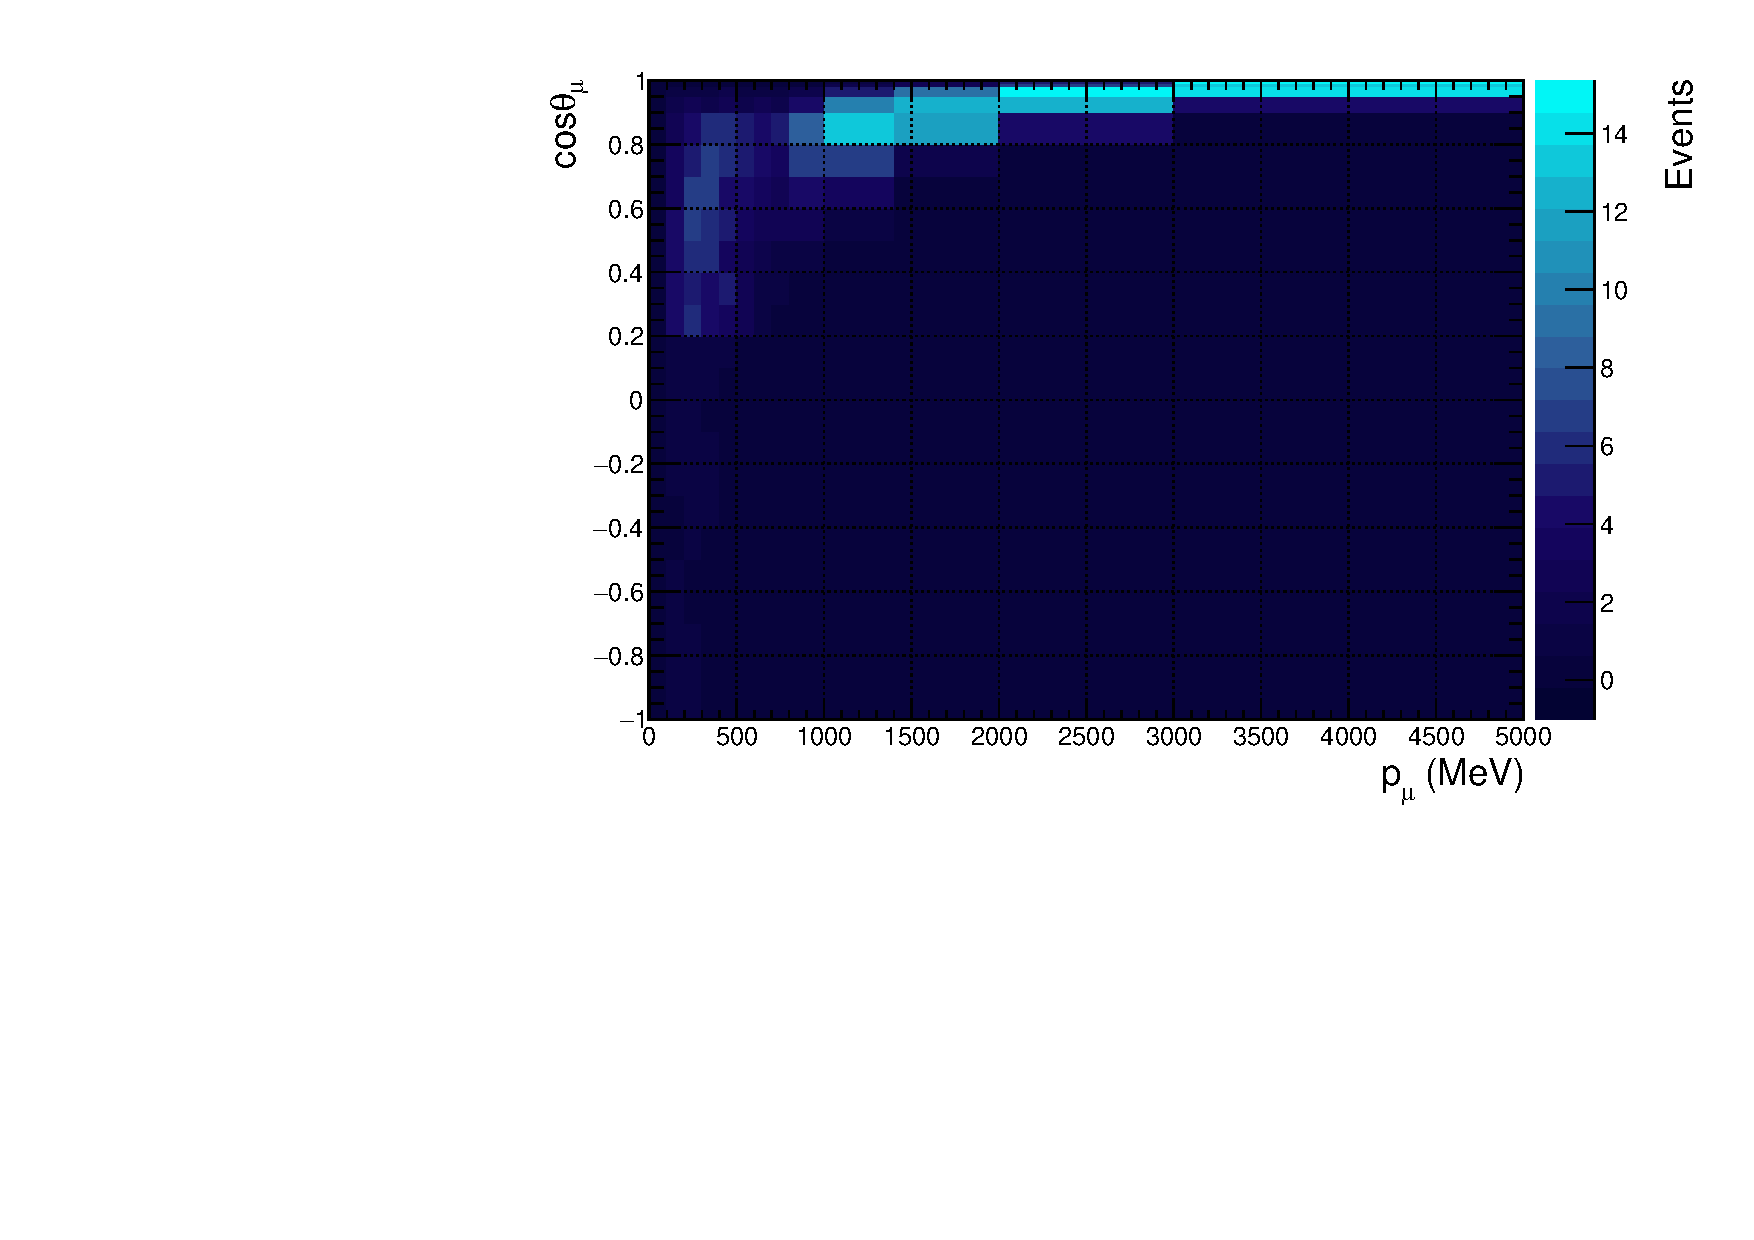
\includegraphics[width=0.9\linewidth]{figs/nd280_pmtmuu_cc0piNp.pdf}
  \caption{CC 0$\pi$ Np}
\end{subfigure}
\begin{subfigure}{.49\textwidth}
  \centering
  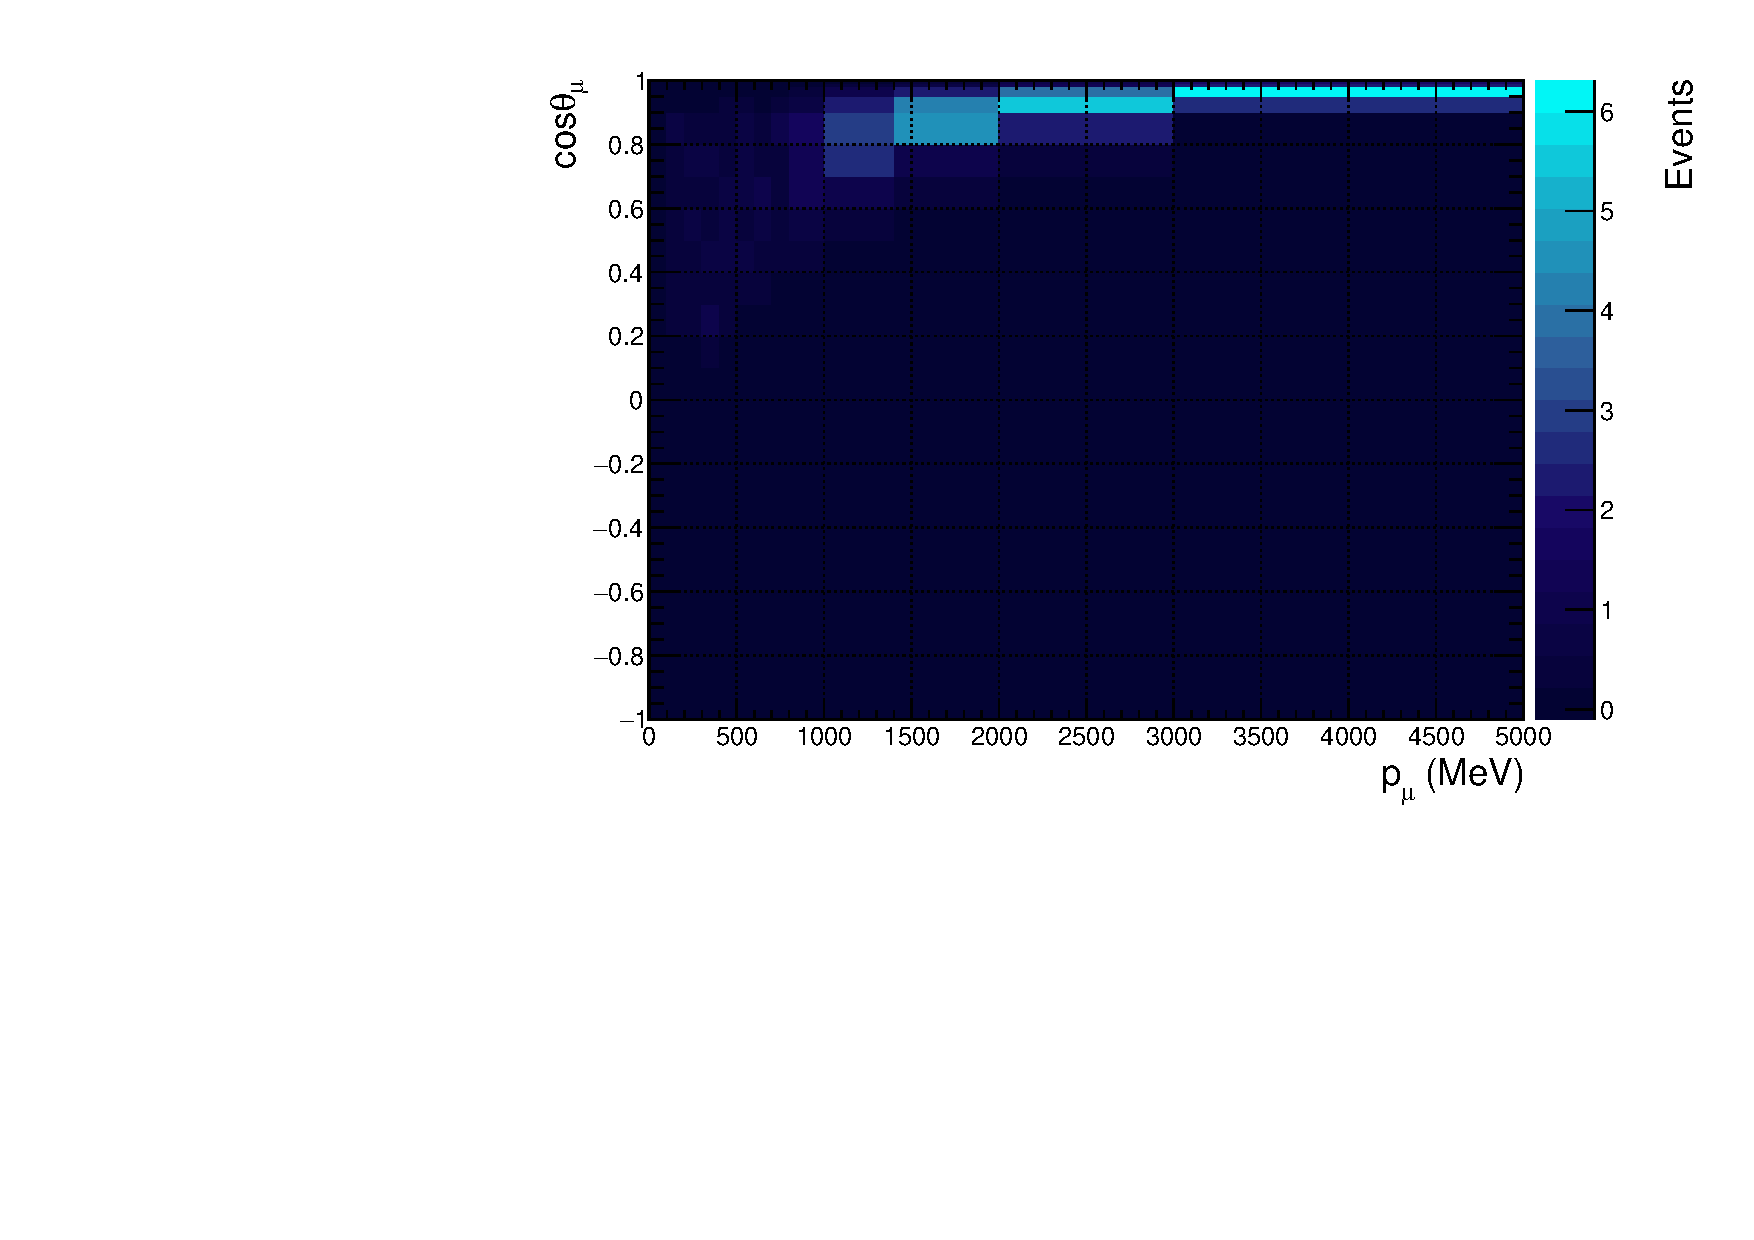
\includegraphics[width=0.9\linewidth]{figs/nd280_pmtmuu_cc1piNp.pdf}
  \caption{CC 1$\pi$ Np}
\end{subfigure}
\begin{subfigure}{.49\textwidth}
  \centering
  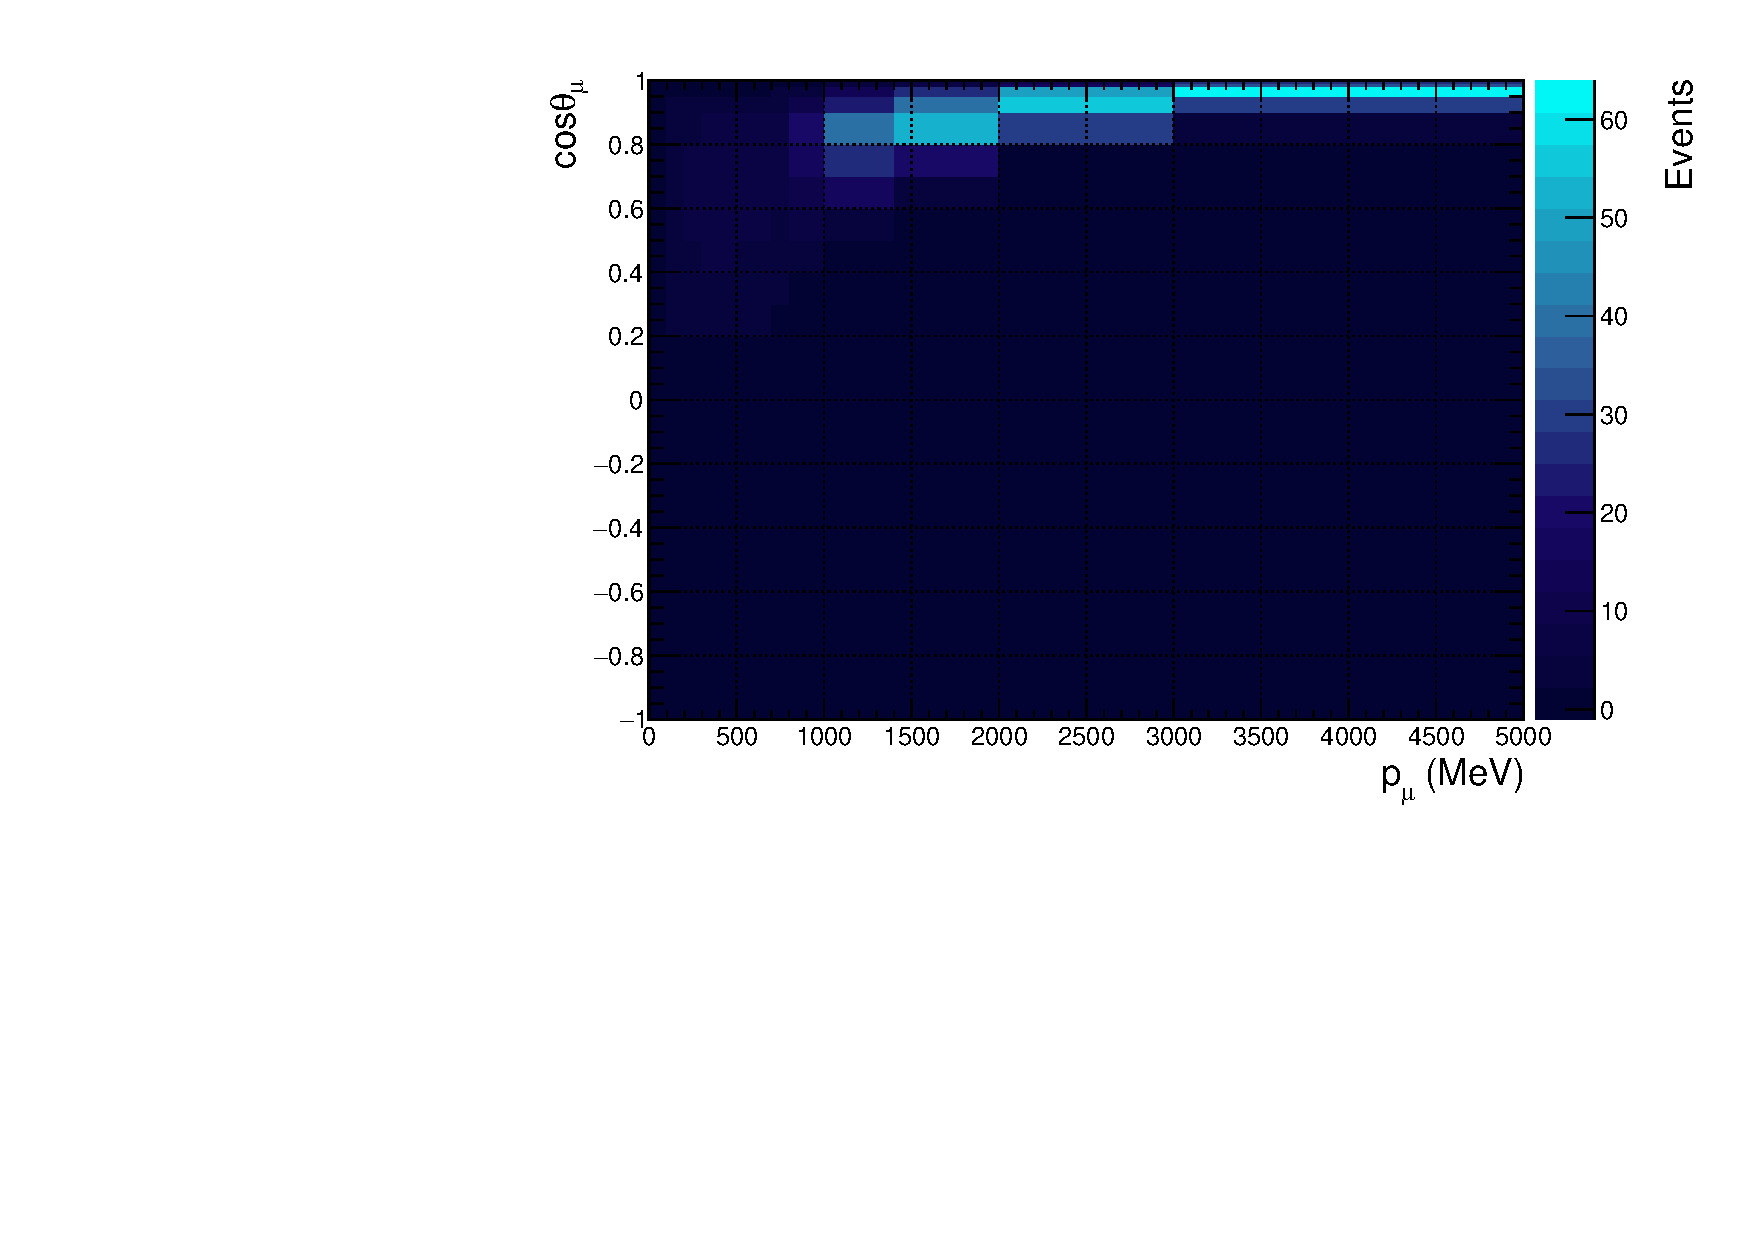
\includegraphics[width=0.9\linewidth]{figs/nd280_pmtmuu_ccOther.pdf}
  \caption{CC Other}
\end{subfigure}
\caption{True $p_{\mu}$-cos$\theta_{\mu}$ distributions for the ND280 MC.}
\label{fig:nd280PmuTmu}
\end{figure}

\begin{figure}
\centering
\begin{subfigure}{.49\textwidth}
  \centering
  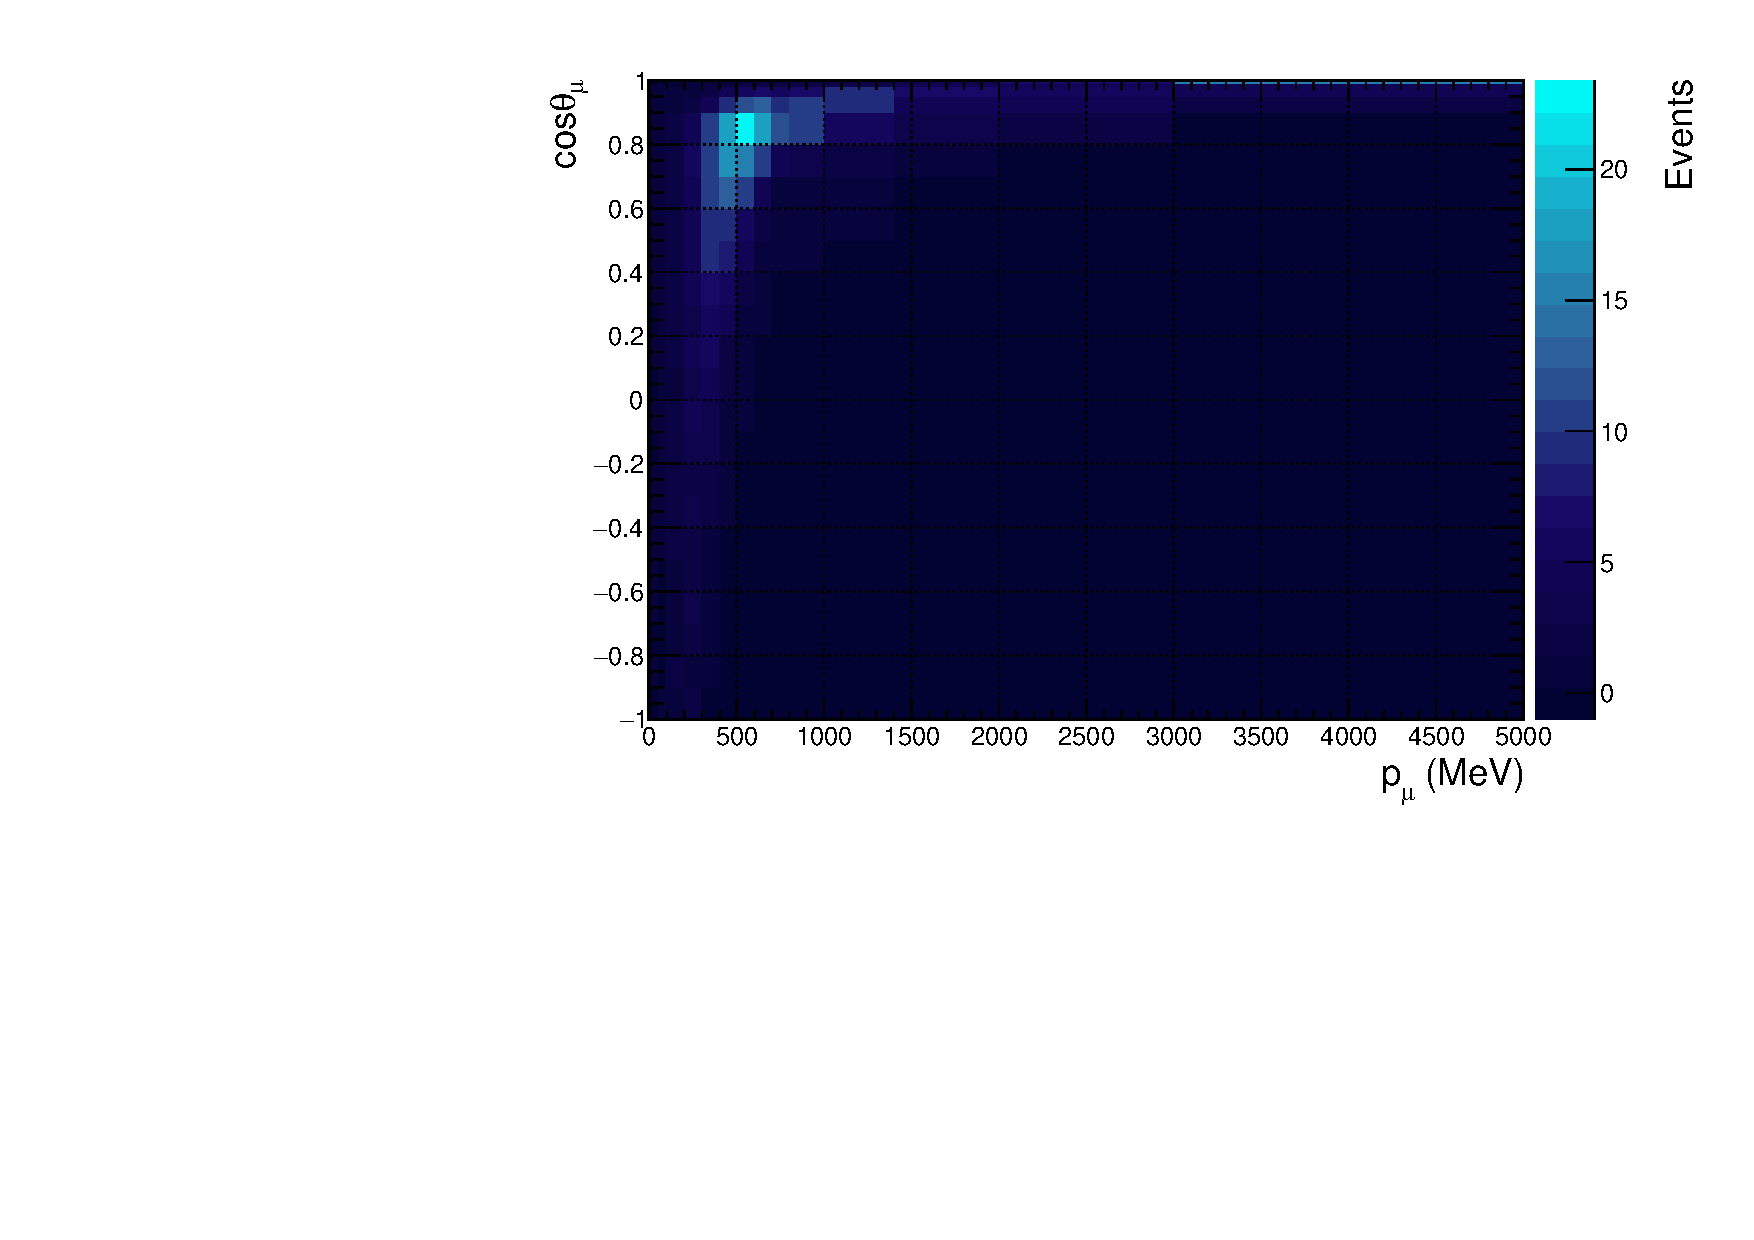
\includegraphics[width=0.9\linewidth]{figs/hptpc_pmtmuu_cc0pi0p.pdf}
  \caption{CC 0$\pi$ 0p}
\end{subfigure}
\begin{subfigure}{.49\textwidth}
  \centering
  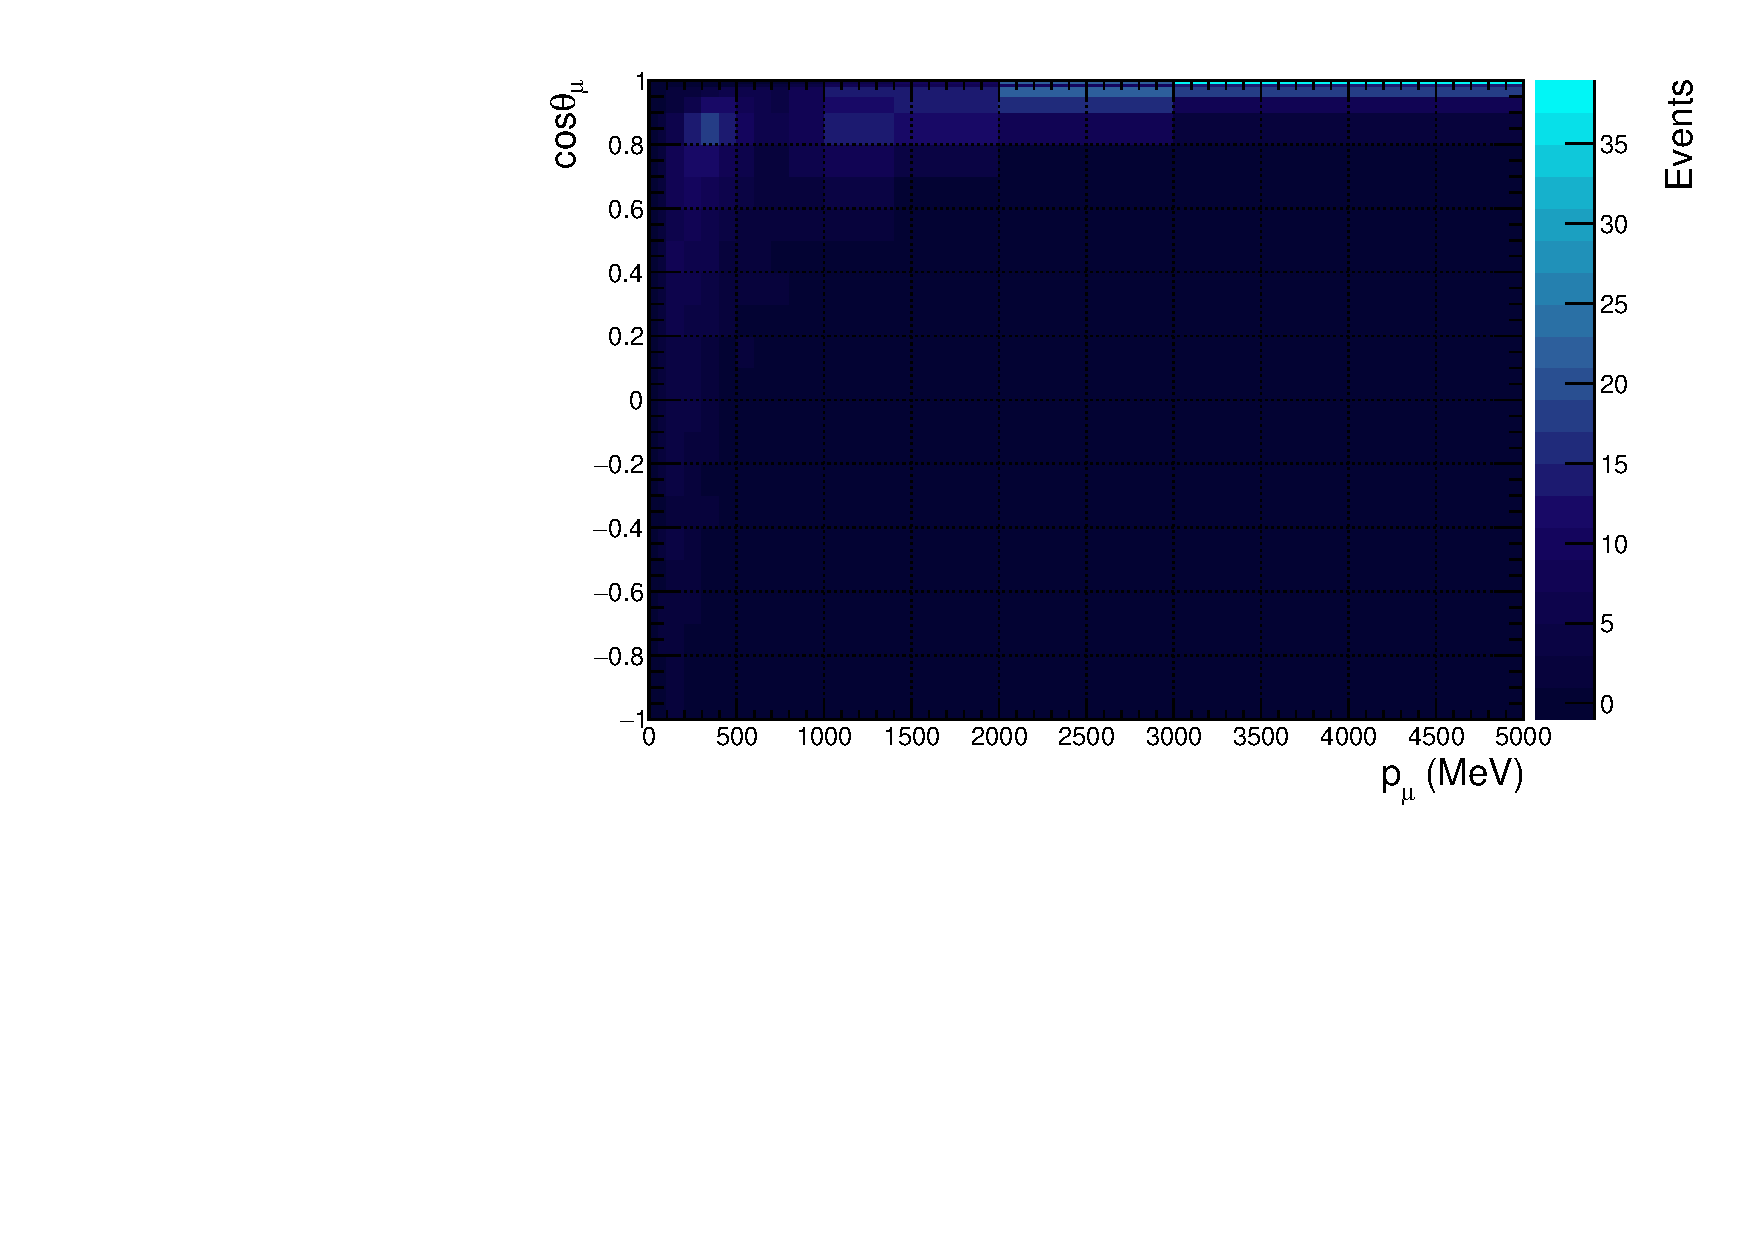
\includegraphics[width=0.9\linewidth]{figs/hptpc_pmtmuu_cc1pi0p.pdf}
  \caption{CC 1$\pi$ 0p}
\end{subfigure}
\begin{subfigure}{.49\textwidth}
  \centering
  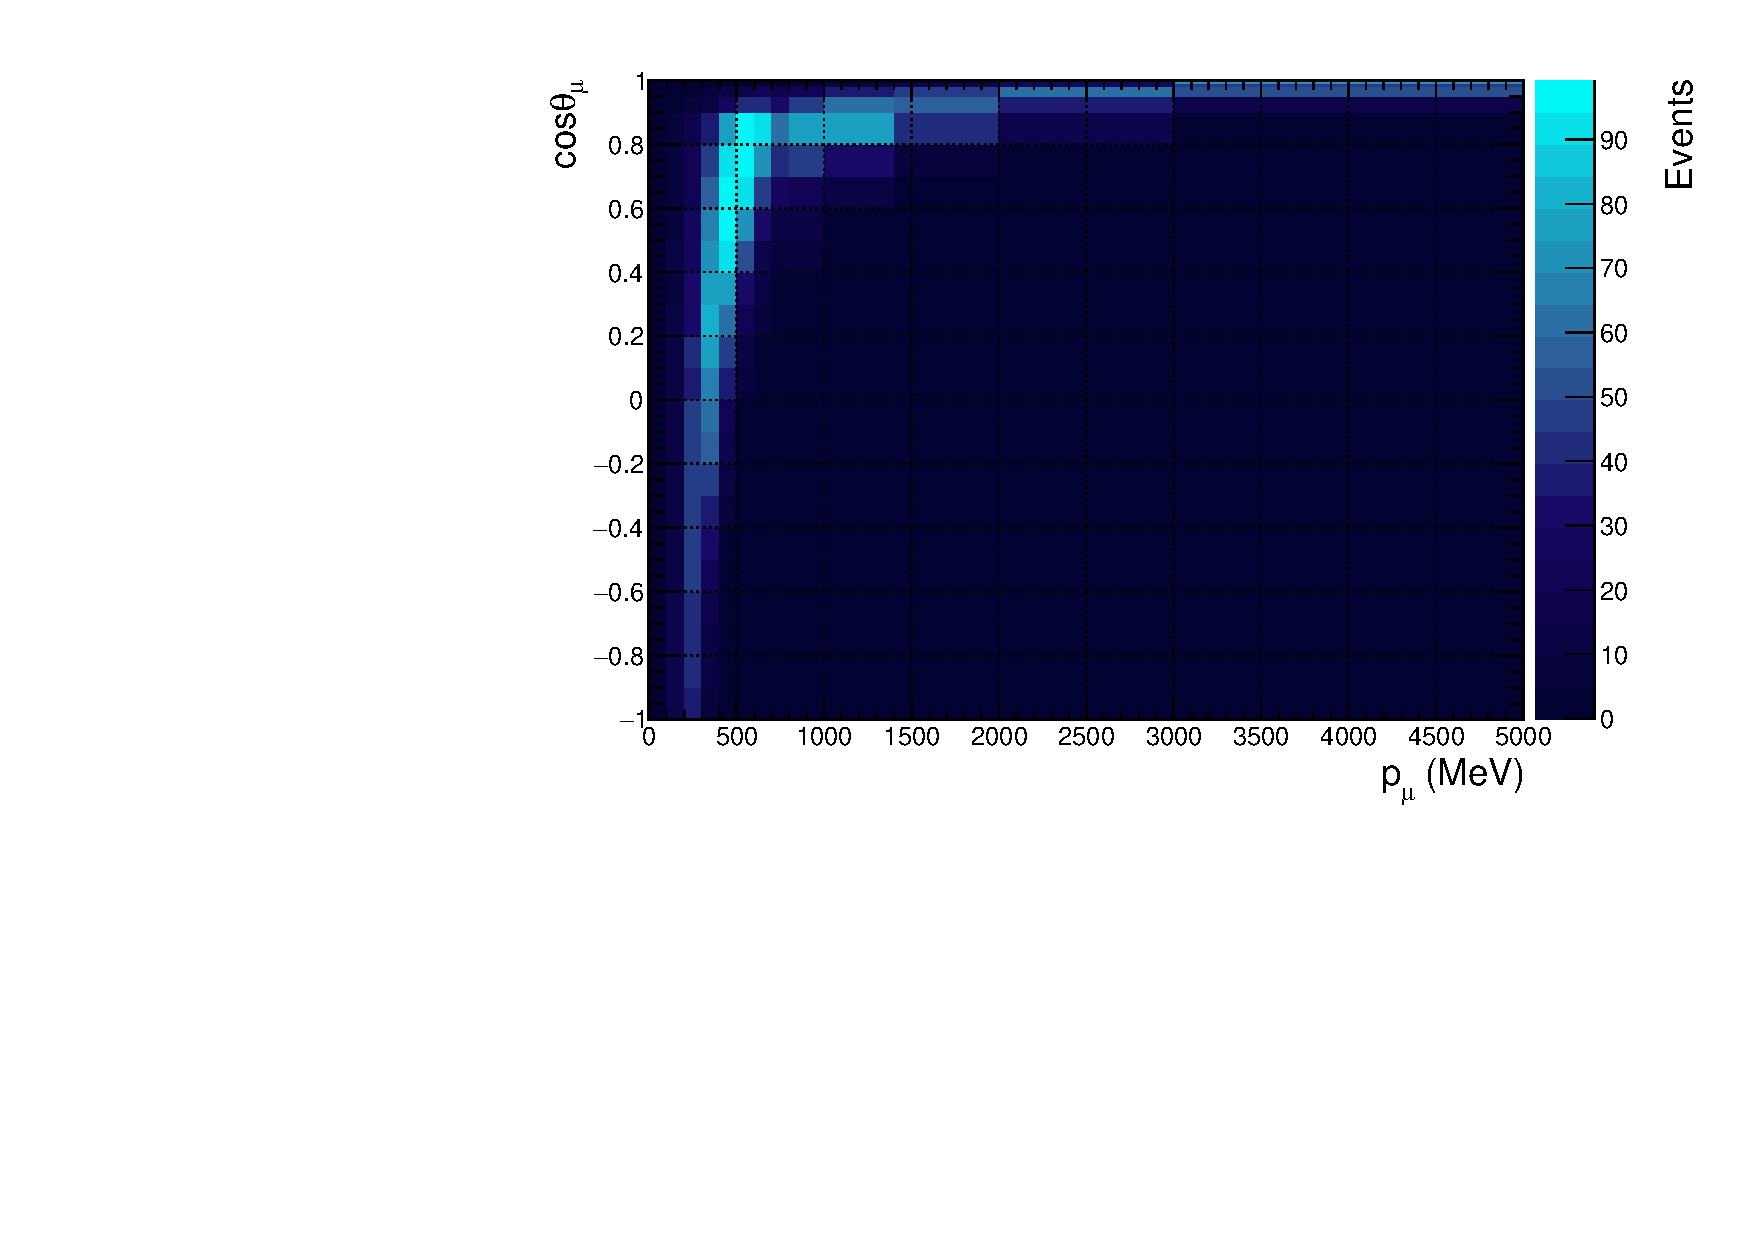
\includegraphics[width=0.9\linewidth]{figs/hptpc_pmtmuu_cc0pi1p.pdf}
  \caption{CC 0$\pi$ 1p}
\end{subfigure}
\begin{subfigure}{.49\textwidth}
  \centering
  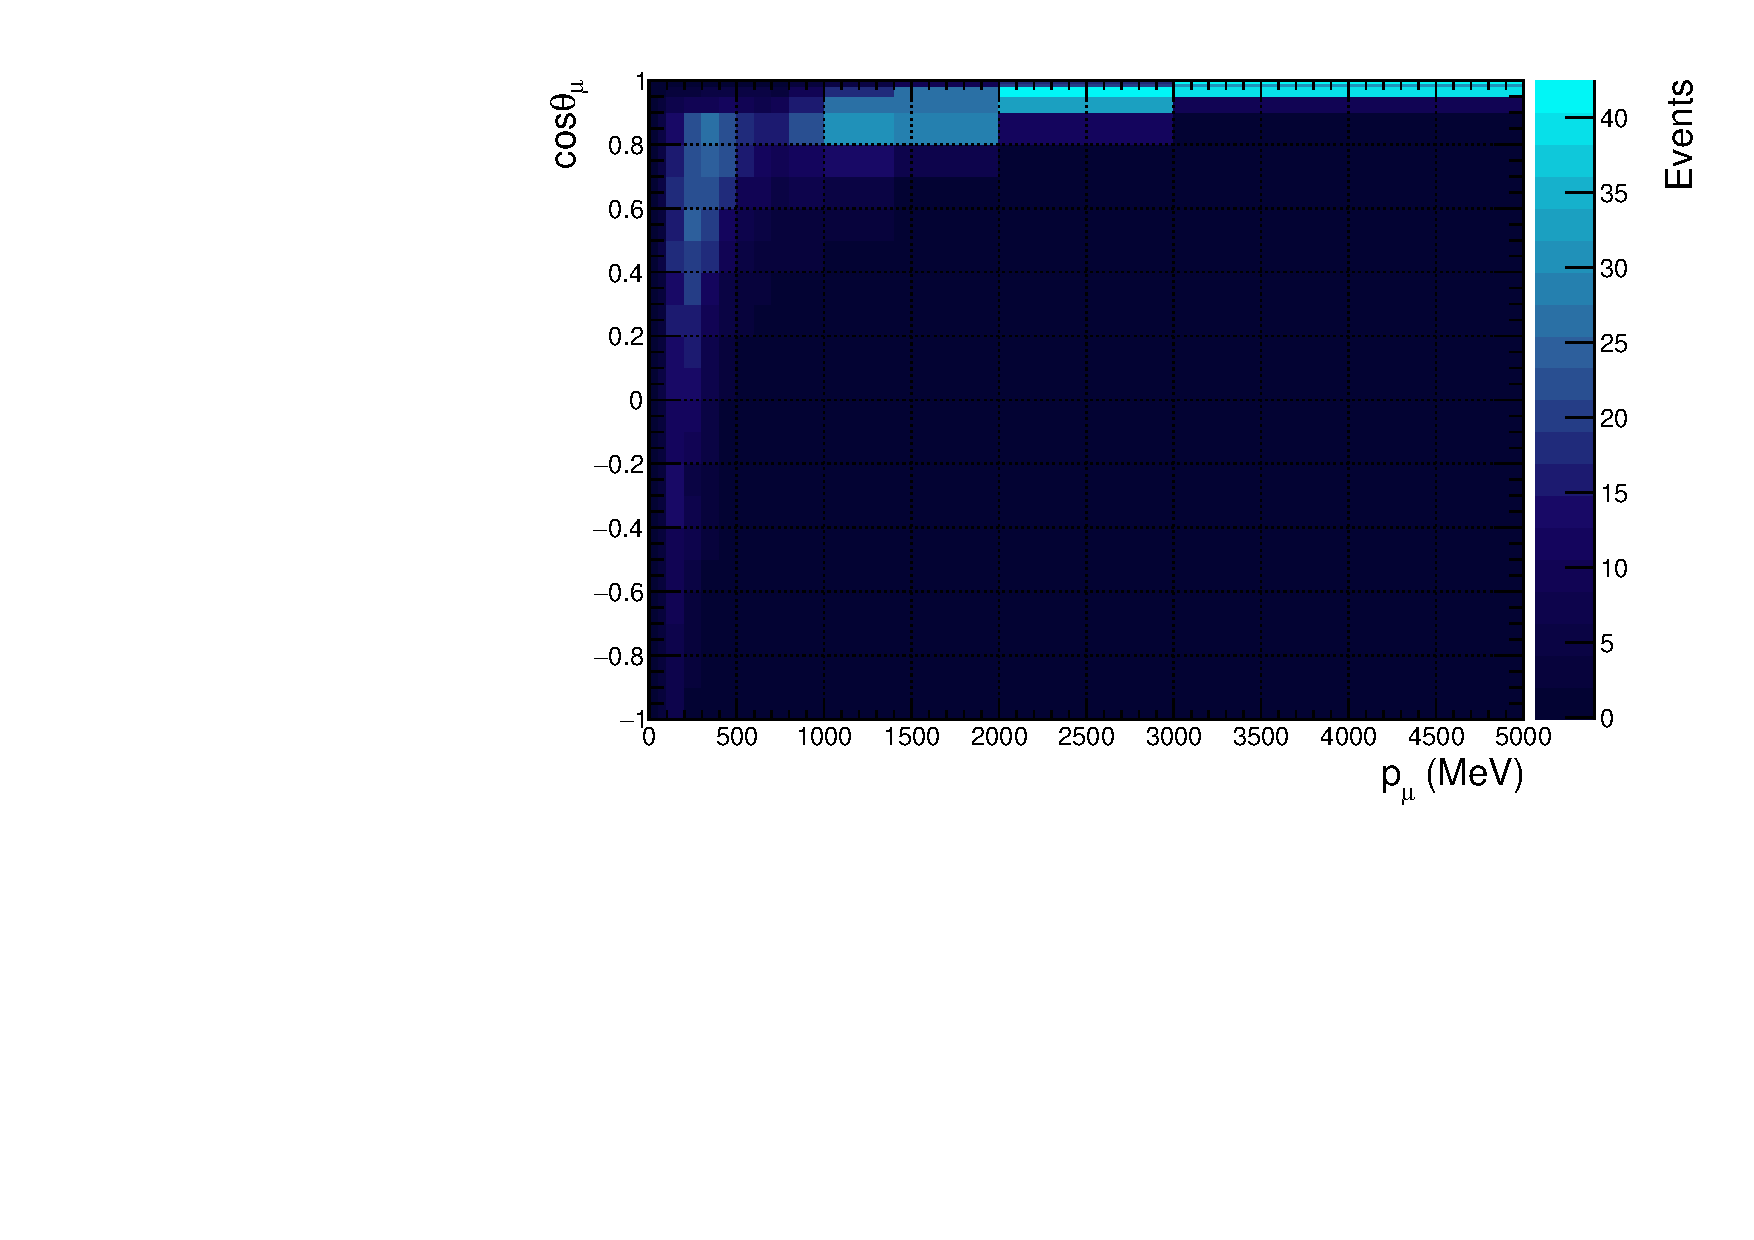
\includegraphics[width=0.9\linewidth]{figs/hptpc_pmtmuu_cc1pi1p.pdf}
  \caption{CC 1$\pi$ 1p}
\end{subfigure}
\begin{subfigure}{.49\textwidth}
  \centering
  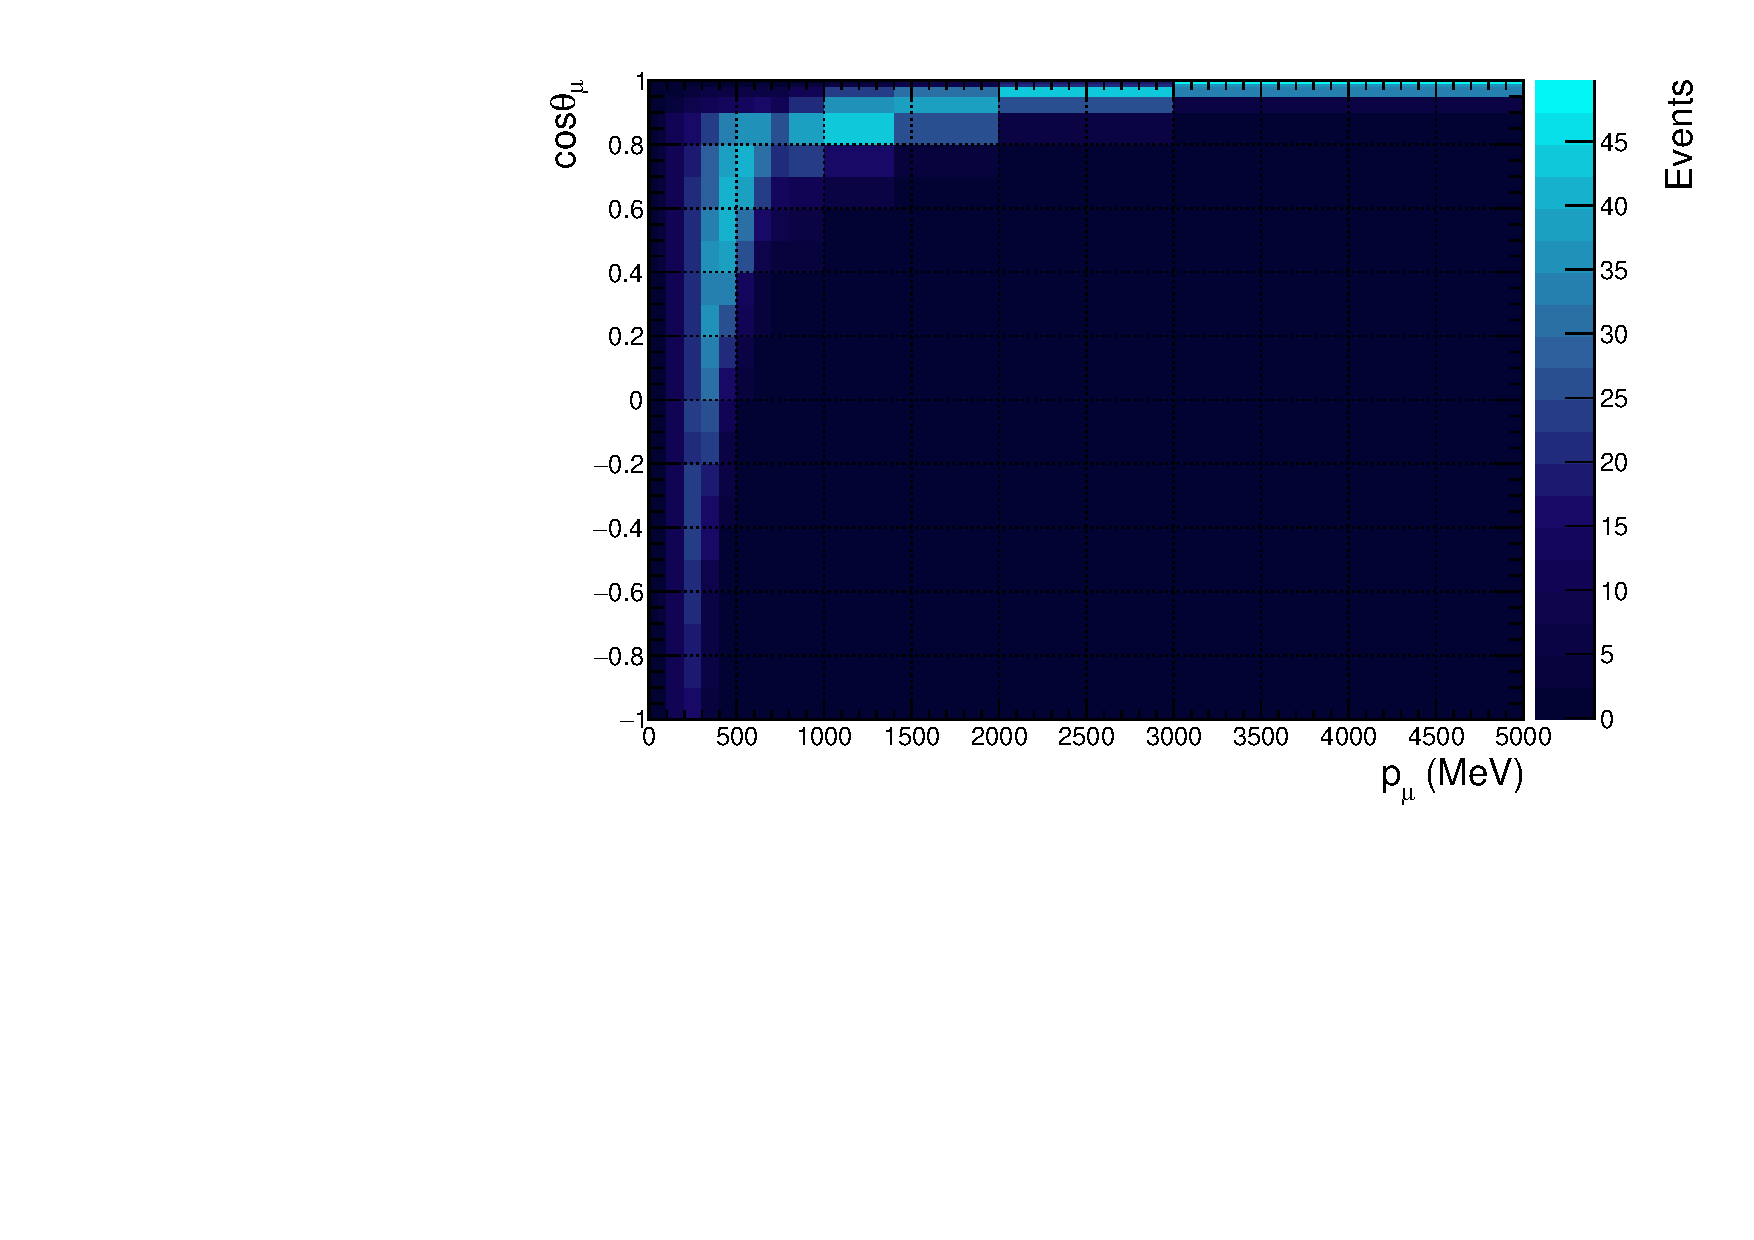
\includegraphics[width=0.9\linewidth]{figs/hptpc_pmtmuu_cc0piNp.pdf}
  \caption{CC 0$\pi$ Np}
\end{subfigure}
\begin{subfigure}{.49\textwidth}
  \centering
  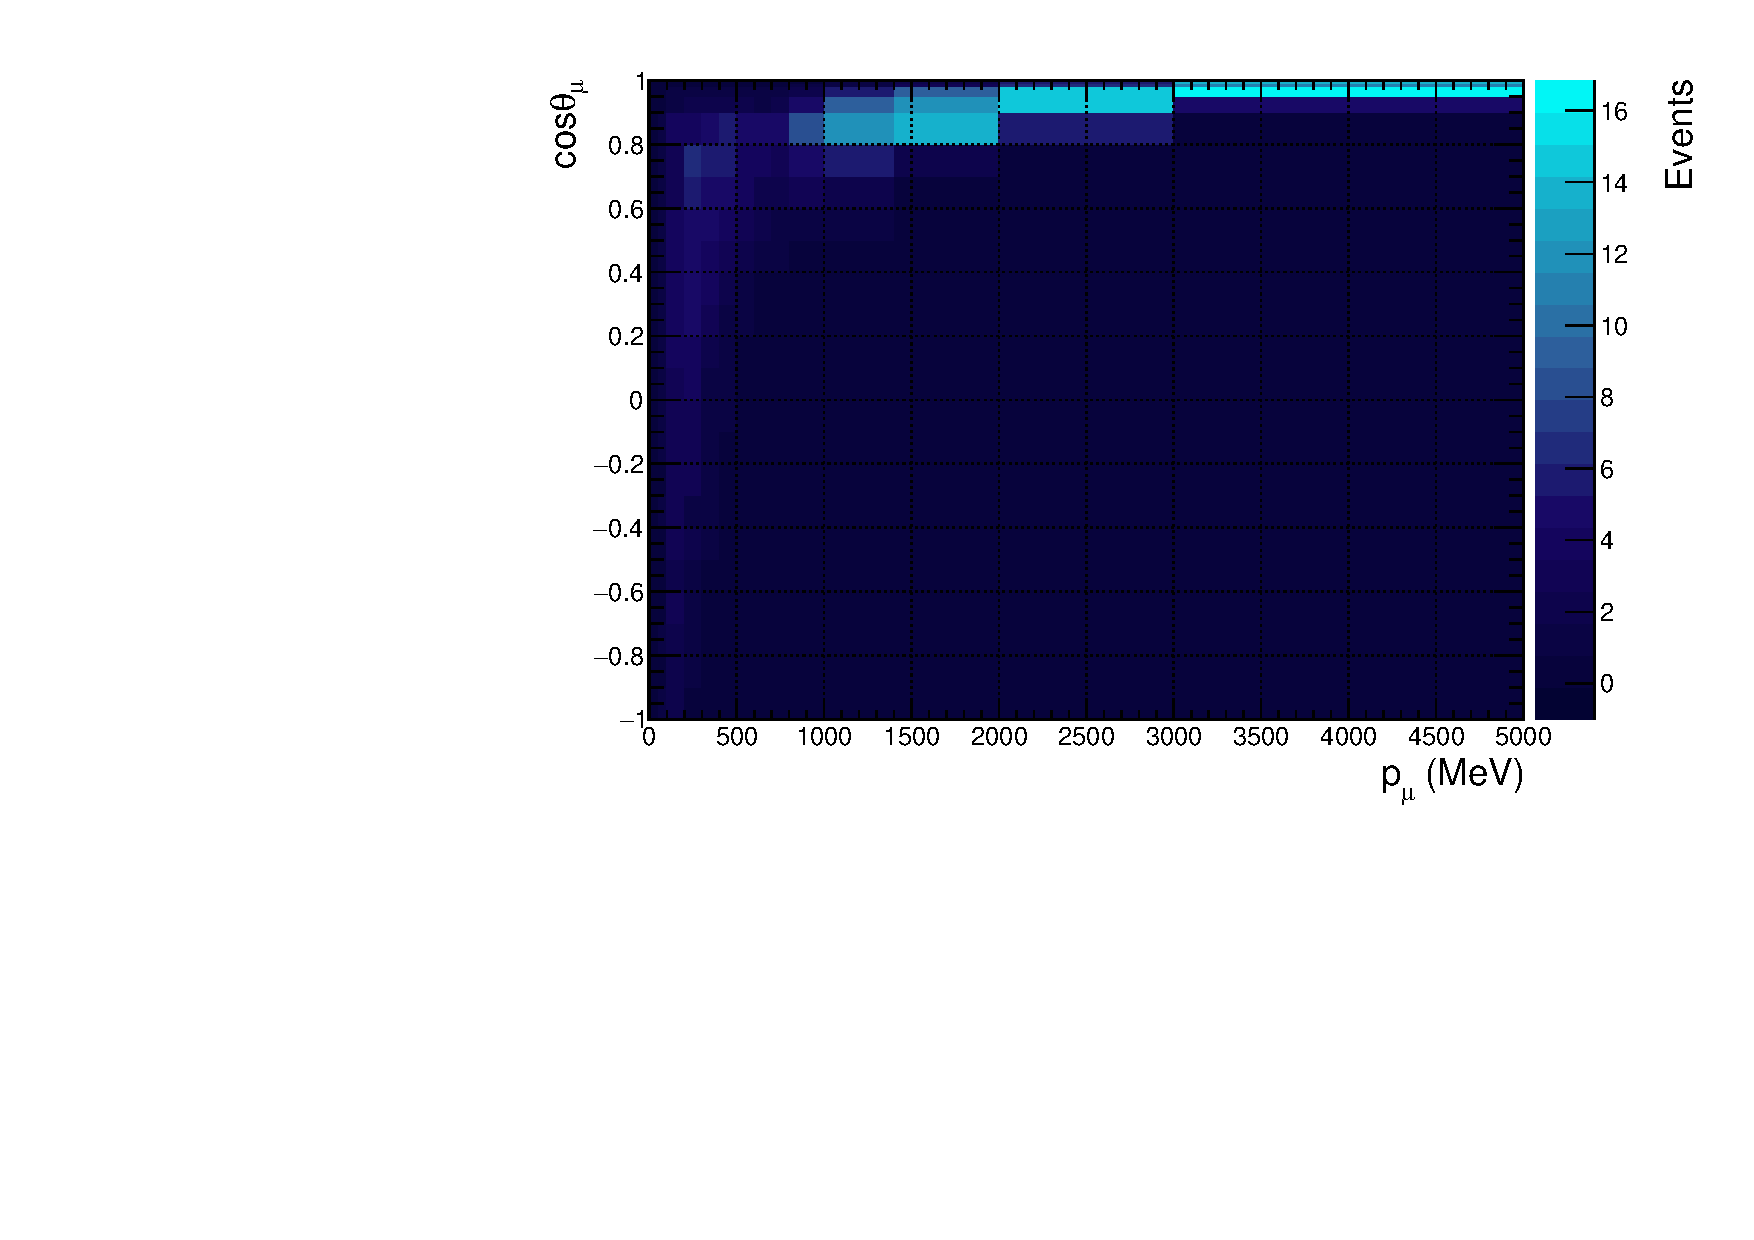
\includegraphics[width=0.9\linewidth]{figs/hptpc_pmtmuu_cc1piNp.pdf}
  \caption{CC 1$\pi$ Np}
\end{subfigure}
\begin{subfigure}{.49\textwidth}
  \centering
  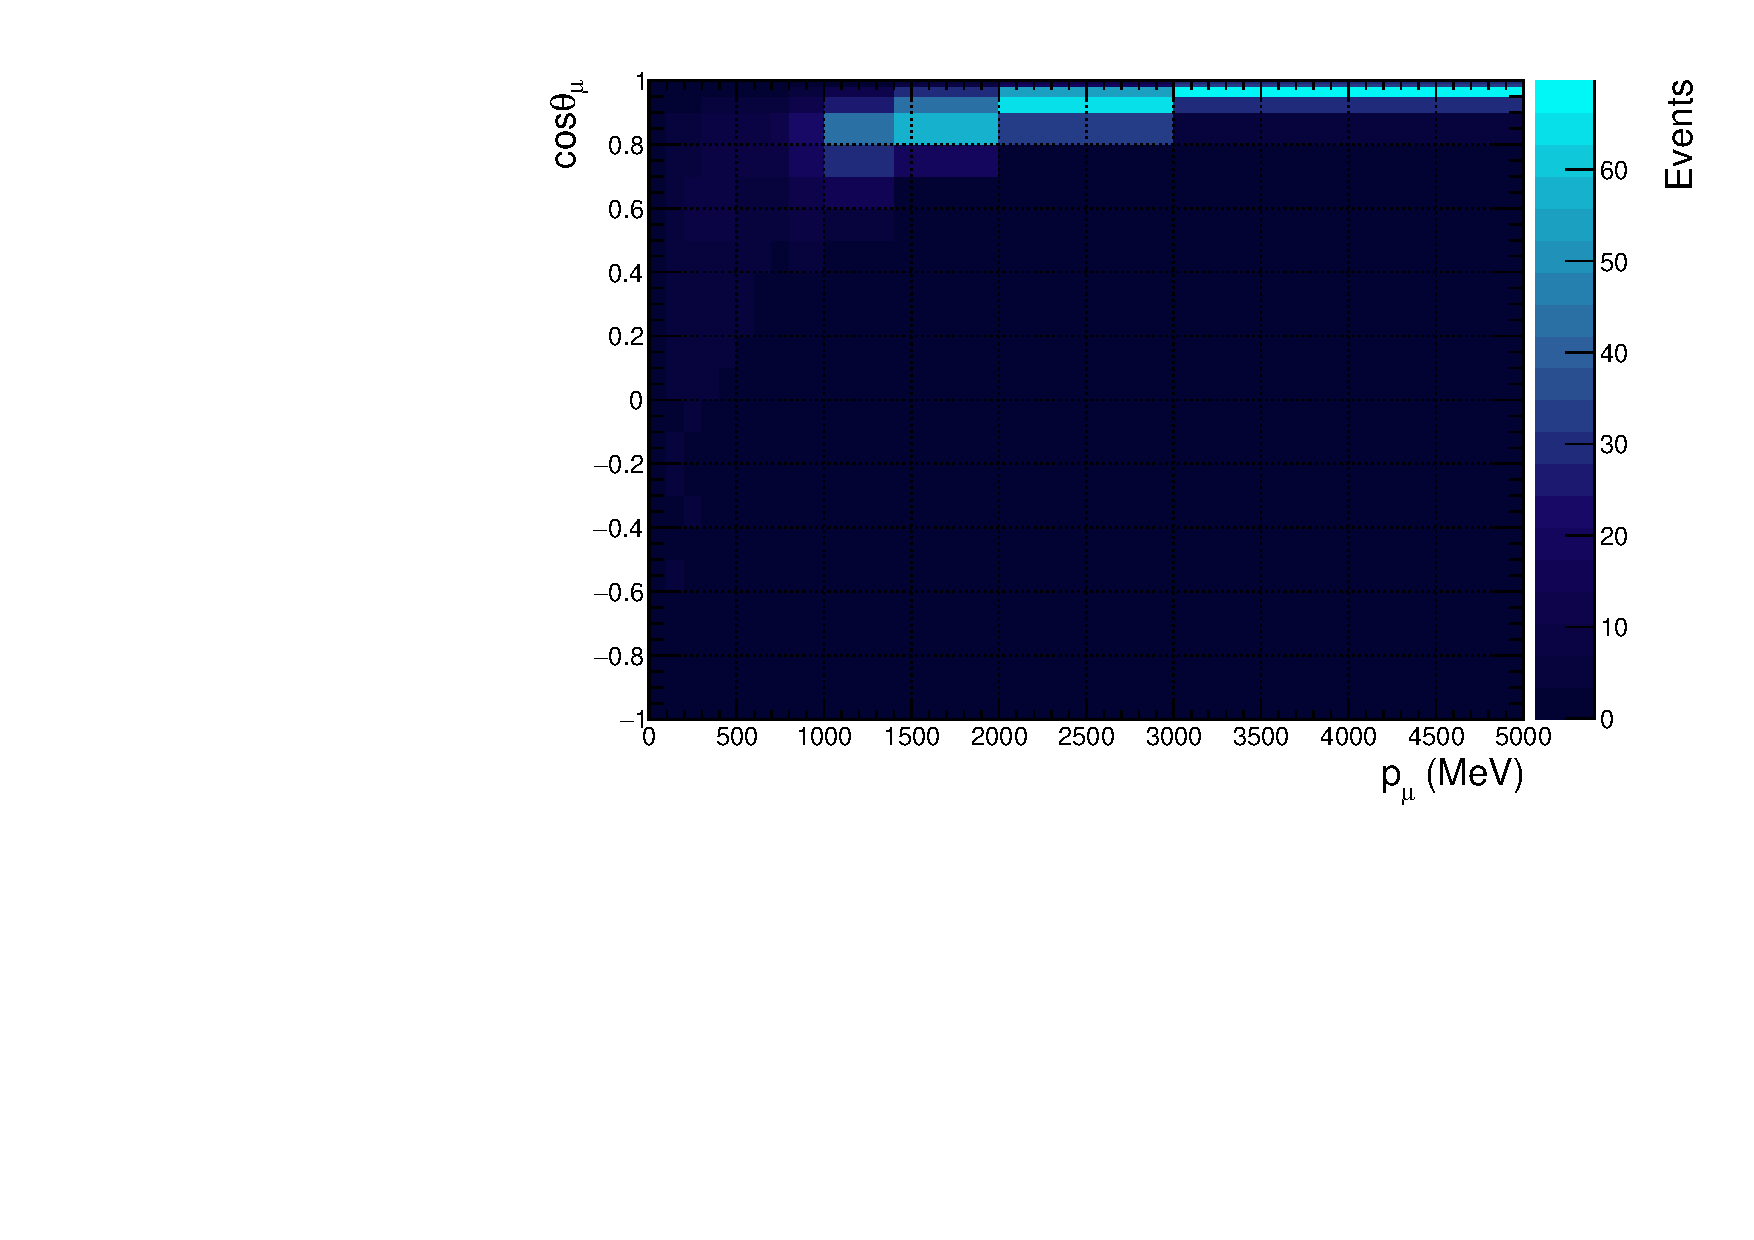
\includegraphics[width=0.9\linewidth]{figs/hptpc_pmtmuu_ccOther.pdf}
  \caption{CC Other}
\end{subfigure}
\caption{True $p_{\mu}$-cos$\theta_{\mu}$ distributions for the HPTPC MC.}
\label{fig:hptpcPmuTmu}
\end{figure}

The distributions of CC 0$\pi$ 0p and CC 0$\pi$ 1p samples are similar for the two detectors, but the normalisations are higher for ND280. The 1p and Np samples have significantly more backward going low momentum events in the HPTPC distributions than ND280. This is because if a proton is detected in an event with a low momentum lepton, the proton momentum is also likely to be low, and so more will be below the ND280 detection threshold. The shape of the CC Other distributions are similar, but there is a slightly higher normalisation for HPTPC.

The full potential sensitivity of the HPTPC to resolving nuclear model tensions cannot be achieved with lepton kinematics alone. To investigate the impact of using hadronic information in interactions, $\pm1\sigma$ parameter variations were run on the HPTPC MC in different combinations of single transverse variables, and lepton, proton, and pion momentum and angle. The process was the same as that described in Section \ref{sec:sigvar}, but events were binned in different variables.

The transverse variables are calculated for each event from the smeared true lepton momentum and angle. For each sample, the combination of interaction parameter and kinematic variables which caused the largest changed in the total number of events is shown in Table \ref{tab:hptpcsigvar}. 

\begin{center}
\begin{table}[!htbp]
\center
\begin{tabular}{l ||c c}
\hline \hline
\textbf{Sample} & \textbf{Parameter} & \textbf{Kinematic Variables} \\
 \hline \hline
CC 0$\pi$ 0p & $M_{A}^{RES}$ & $p_{\mu}$-cos$\theta_{\mu}$\\
CC 0$\pi$ 1p & 2p2h Shape C & $p_{p}$-cos$\theta_{\mu}$\\
CC 0$\pi$ Np & $M_{A}^{QE}$ & $p_{p}$-cos$\theta_{\mu}$\\
CC 1$\pi$ 0p & $M_{A}^{RES}$ & $p_{\pi}$-cos$\theta_{\mu}$\\
CC 1$\pi$ 1p & $C_{A}^{5}$ & $\delta p_{T}$-cos$\theta_{\mu}$\\
CC 1$\pi$ Np & $C_{A}^{5}$ & $p_{p}$-cos$\theta_{\mu}$\\
CC Other & CC DIS & $p_{\mu}$-cos$\theta_{\mu}$\\
\hline \hline
\end{tabular}
\caption{Combination of kinematic variable pair and interaction parameter which caused the biggest change in the total event rate for each sample in the $\pm1\sigma$ parameter variations.}
\label{tab:hptpcsigvar}
\end{table}
\end{center}

Interestingly, for each sample one of the pair of kinematic that  variables that cause the biggest change in the event rates in the parameter variations is either the lepton momentum or angle. This is likely because these variables can be measured with the best resolution by the detectors.

The distributions in these pairs of kinematics for the HPTPC MC samples are shown in Figure \ref{fig:hptpcsigvar}.

\begin{figure}
\centering
\begin{subfigure}{.49\textwidth}
  \centering
  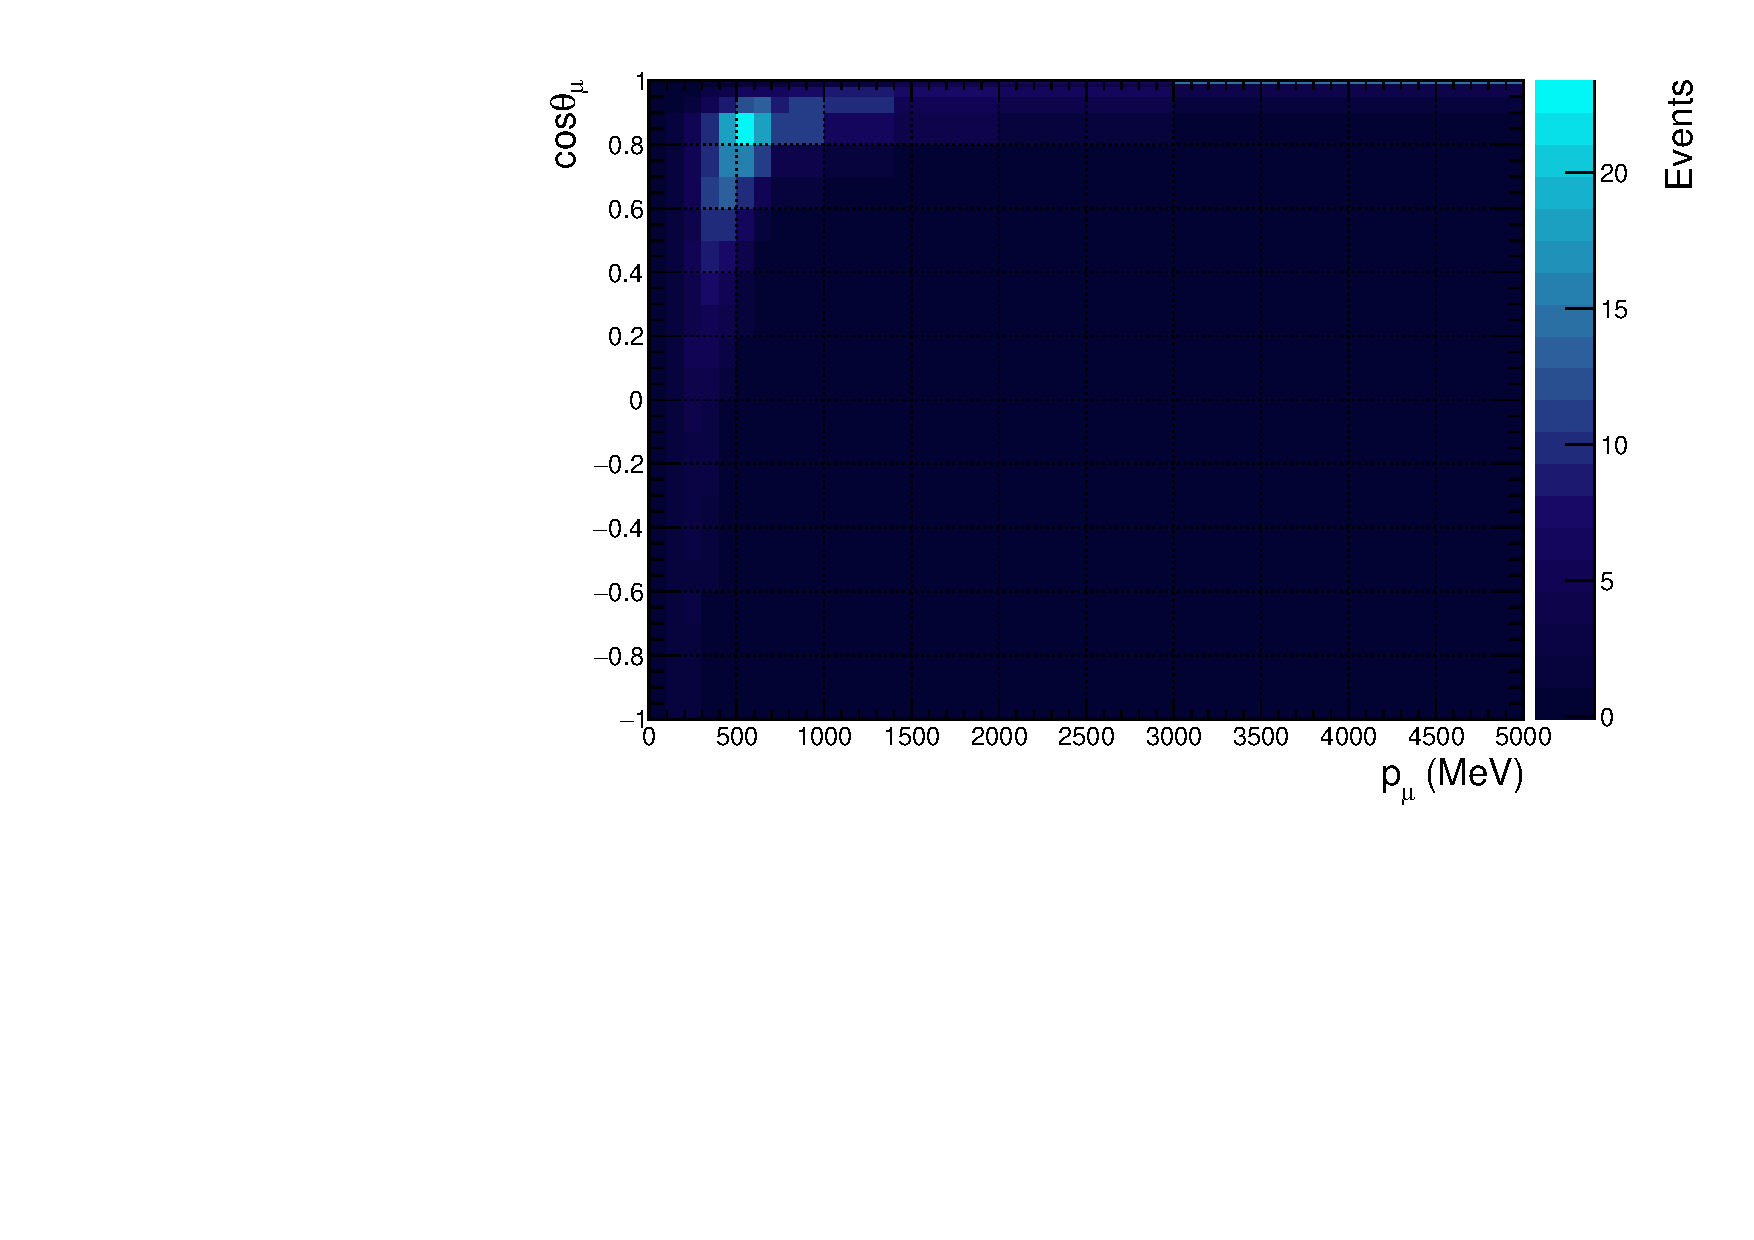
\includegraphics[width=0.9\linewidth]{figs/hptpc_sigvar_cc0pi0p.pdf}
  \caption{CC 0$\pi$ 0p: $p_{\mu}$-cos$\theta_{\mu}$}
\end{subfigure}
\begin{subfigure}{.49\textwidth}
  \centering
  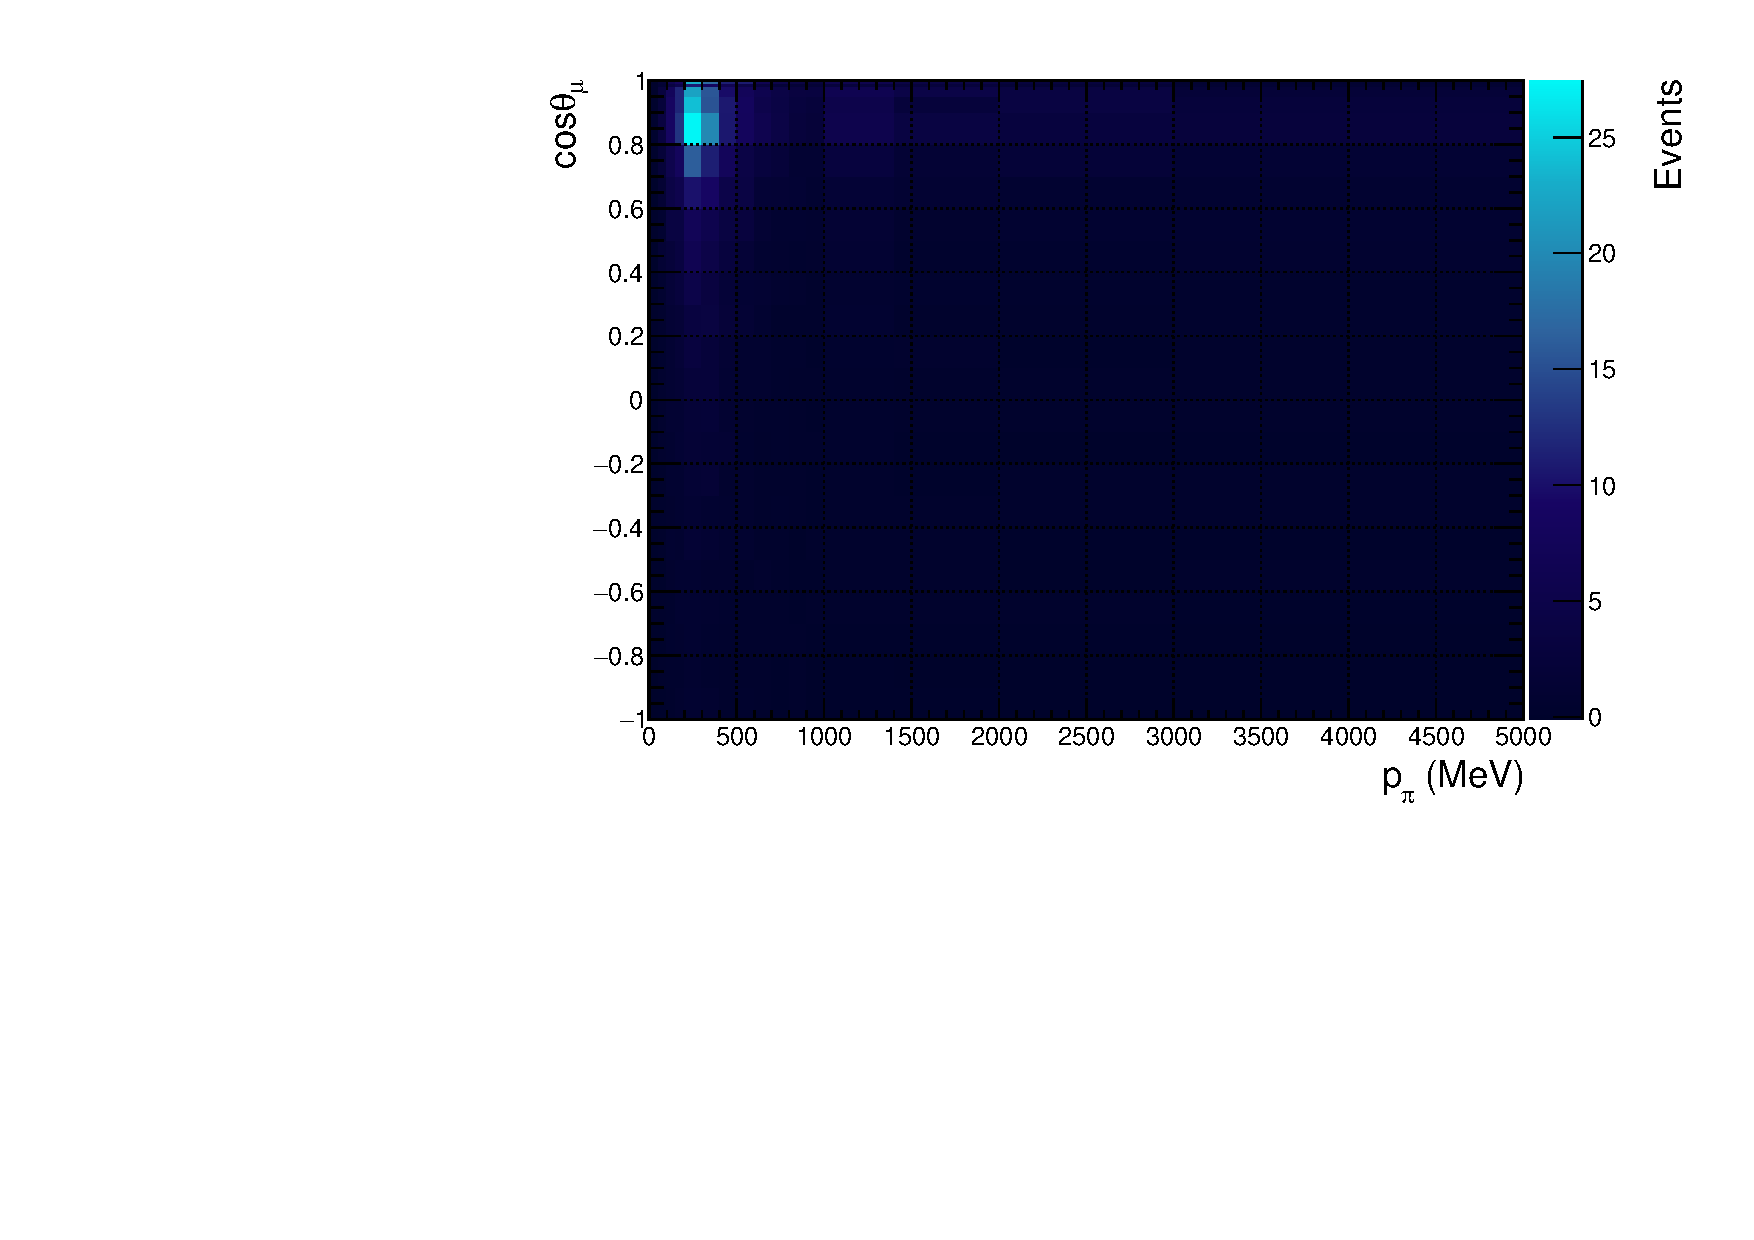
\includegraphics[width=0.9\linewidth]{figs/hptpc_sigvar_cc1pi0p.pdf}
  \caption{CC 1$\pi$ 0p: $p_{\pi}$-cos$\theta_{\mu}$}
\end{subfigure}
\begin{subfigure}{.49\textwidth}
  \centering
  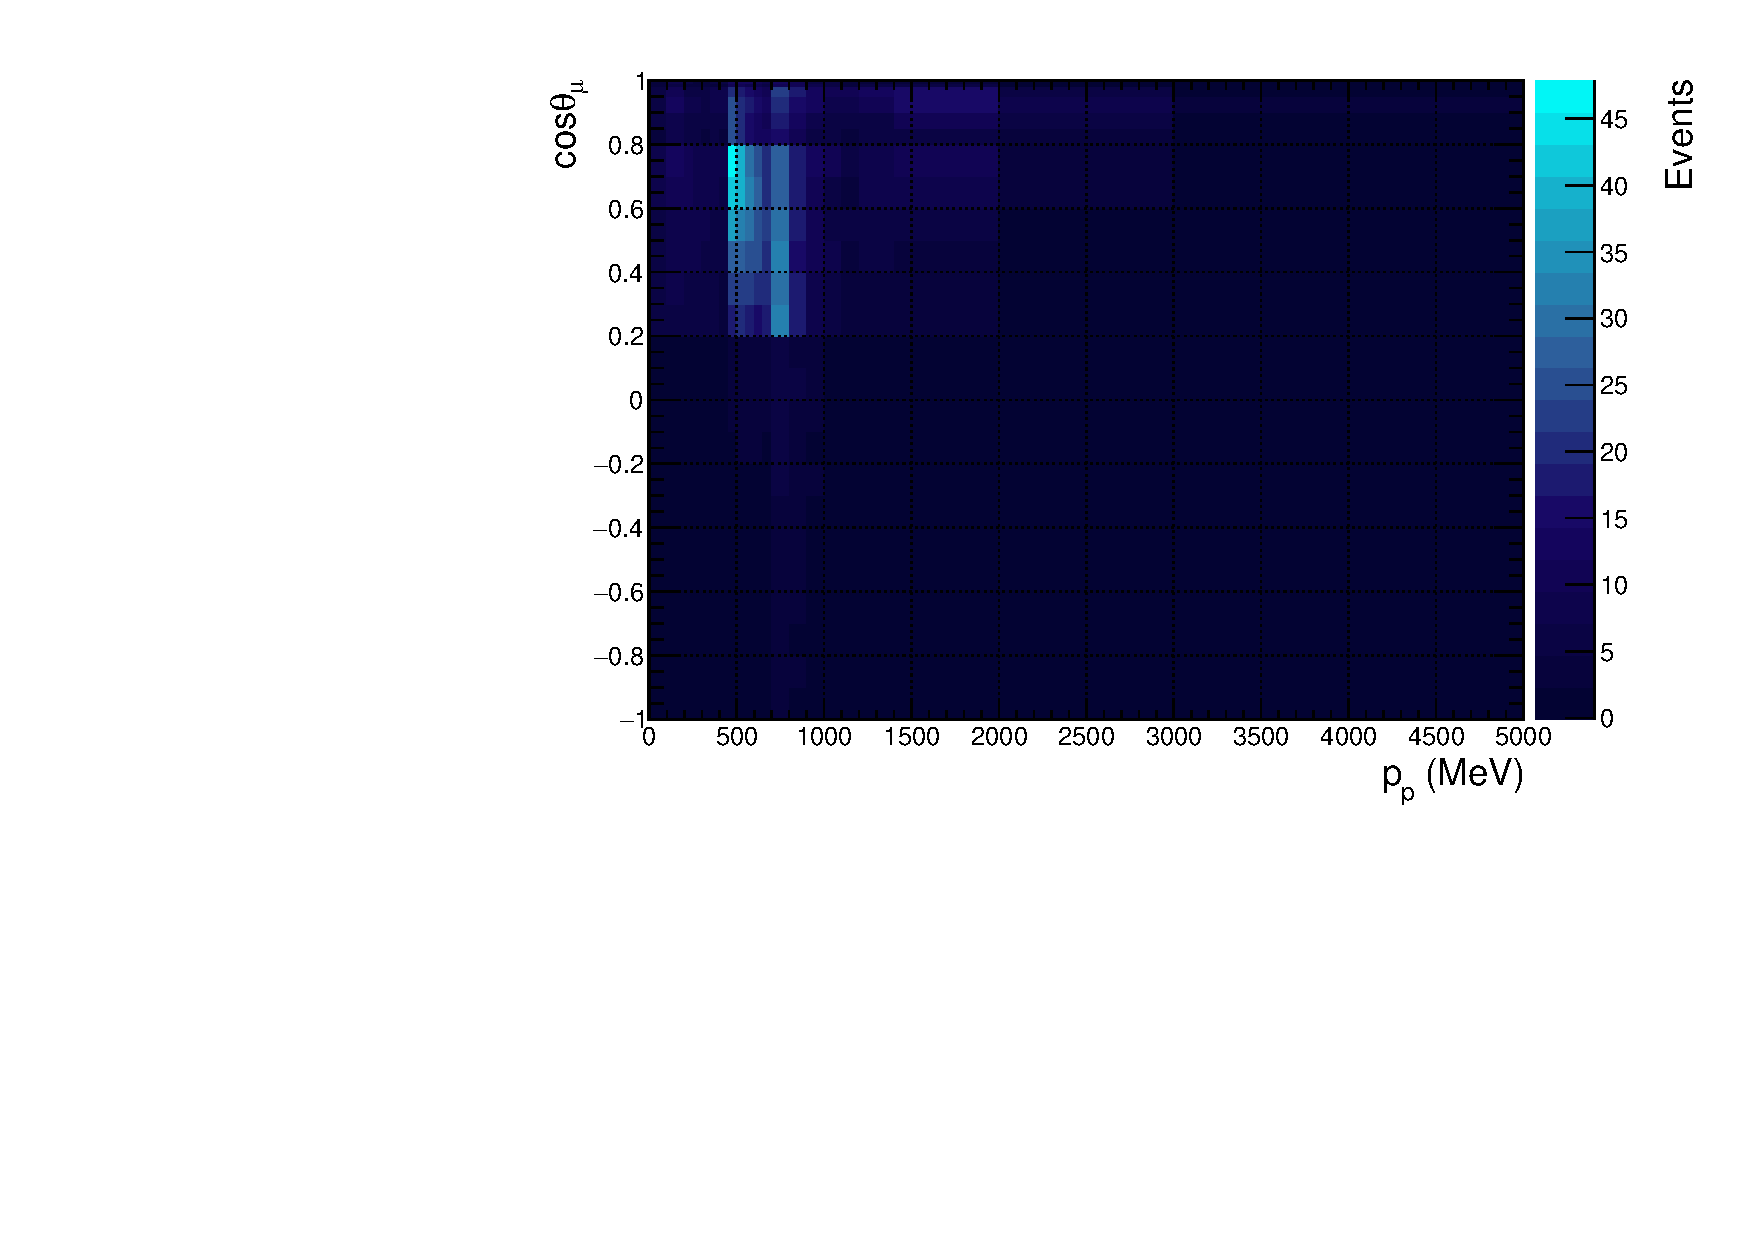
\includegraphics[width=0.9\linewidth]{figs/hptpc_sigvar_cc0pi1p.pdf}
  \caption{CC 0$\pi$ 1p: $p_{p}$-cos$\theta_{\mu}$}
\end{subfigure}
\begin{subfigure}{.49\textwidth}
  \centering
  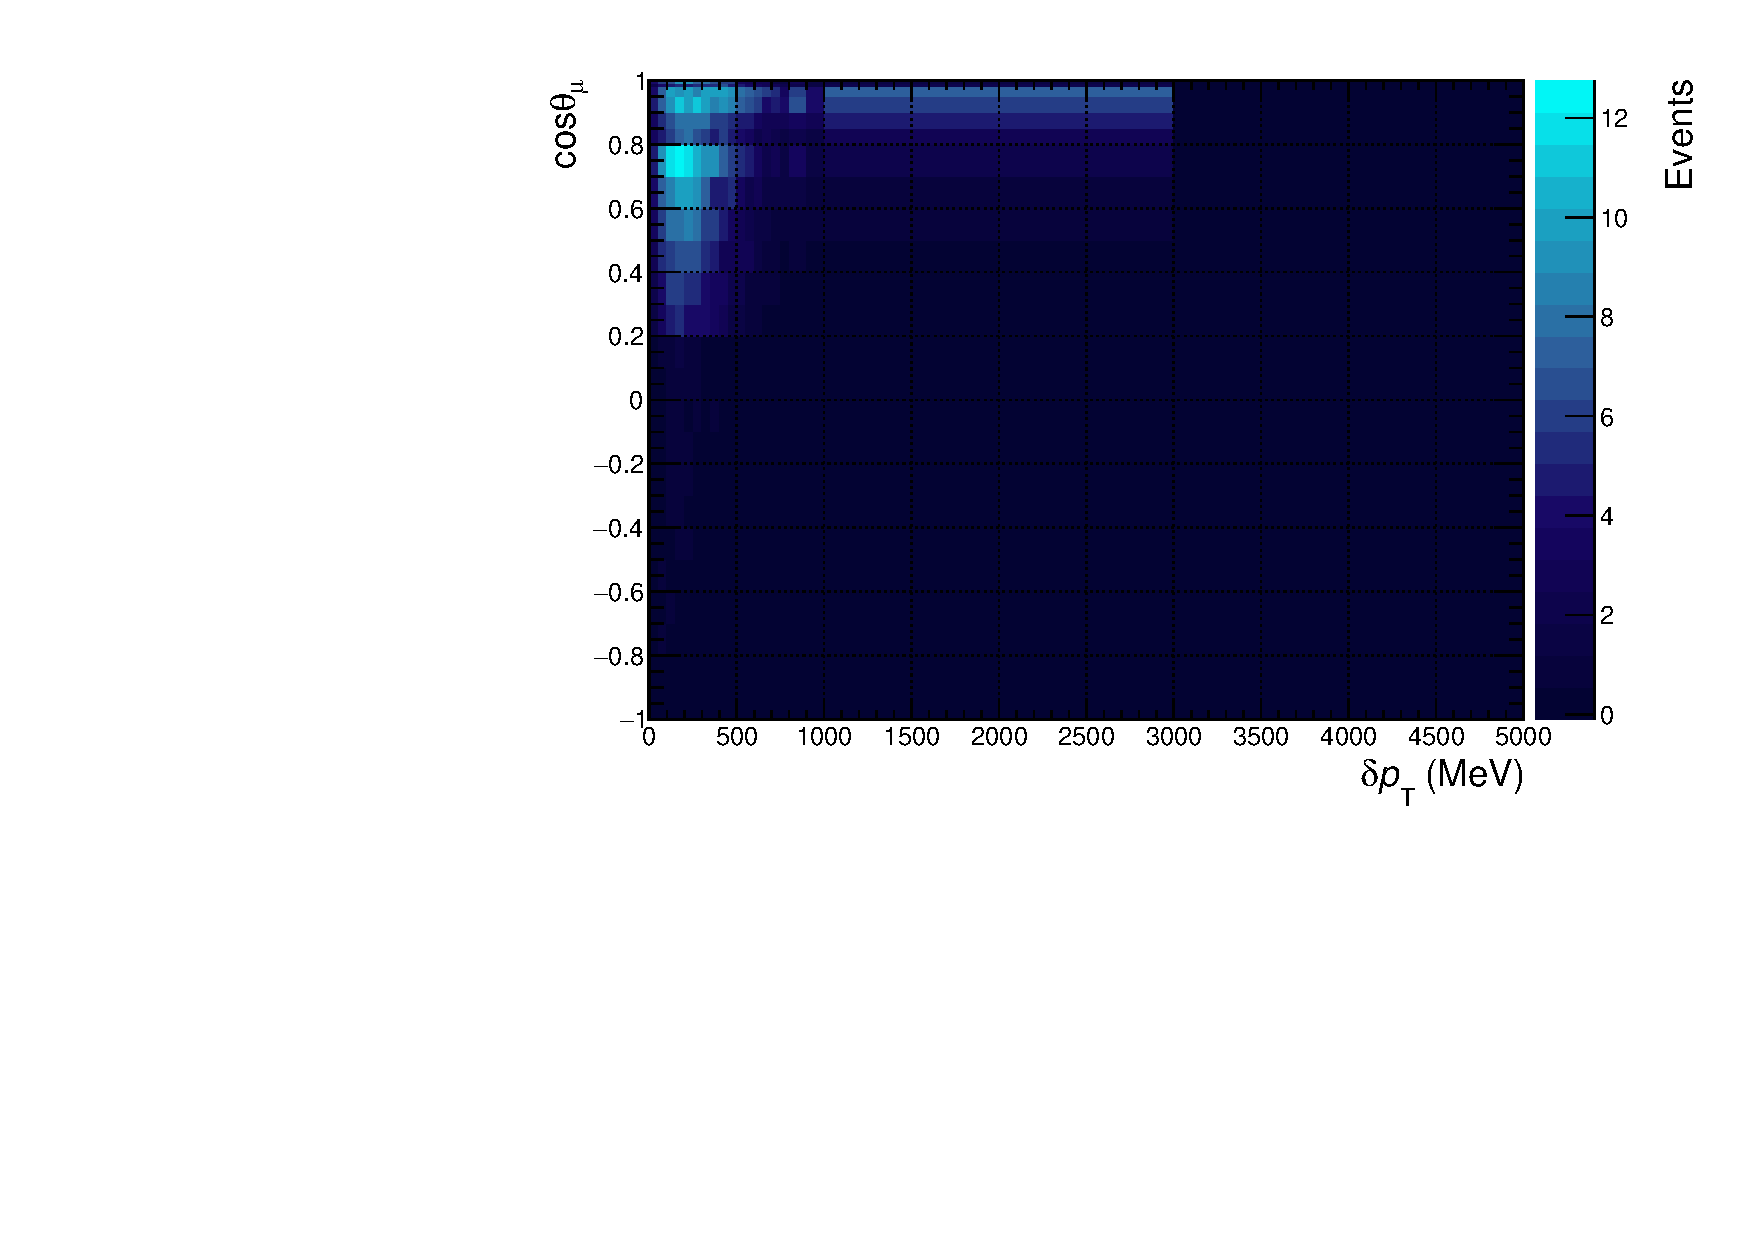
\includegraphics[width=0.9\linewidth]{figs/hptpc_sigvar_cc1pi1p.pdf}
  \caption{CC 1$\pi$ 1p: $\delta p_{T}$-cos$\theta_{\mu}$}
\end{subfigure}
\begin{subfigure}{.49\textwidth}
  \centering
  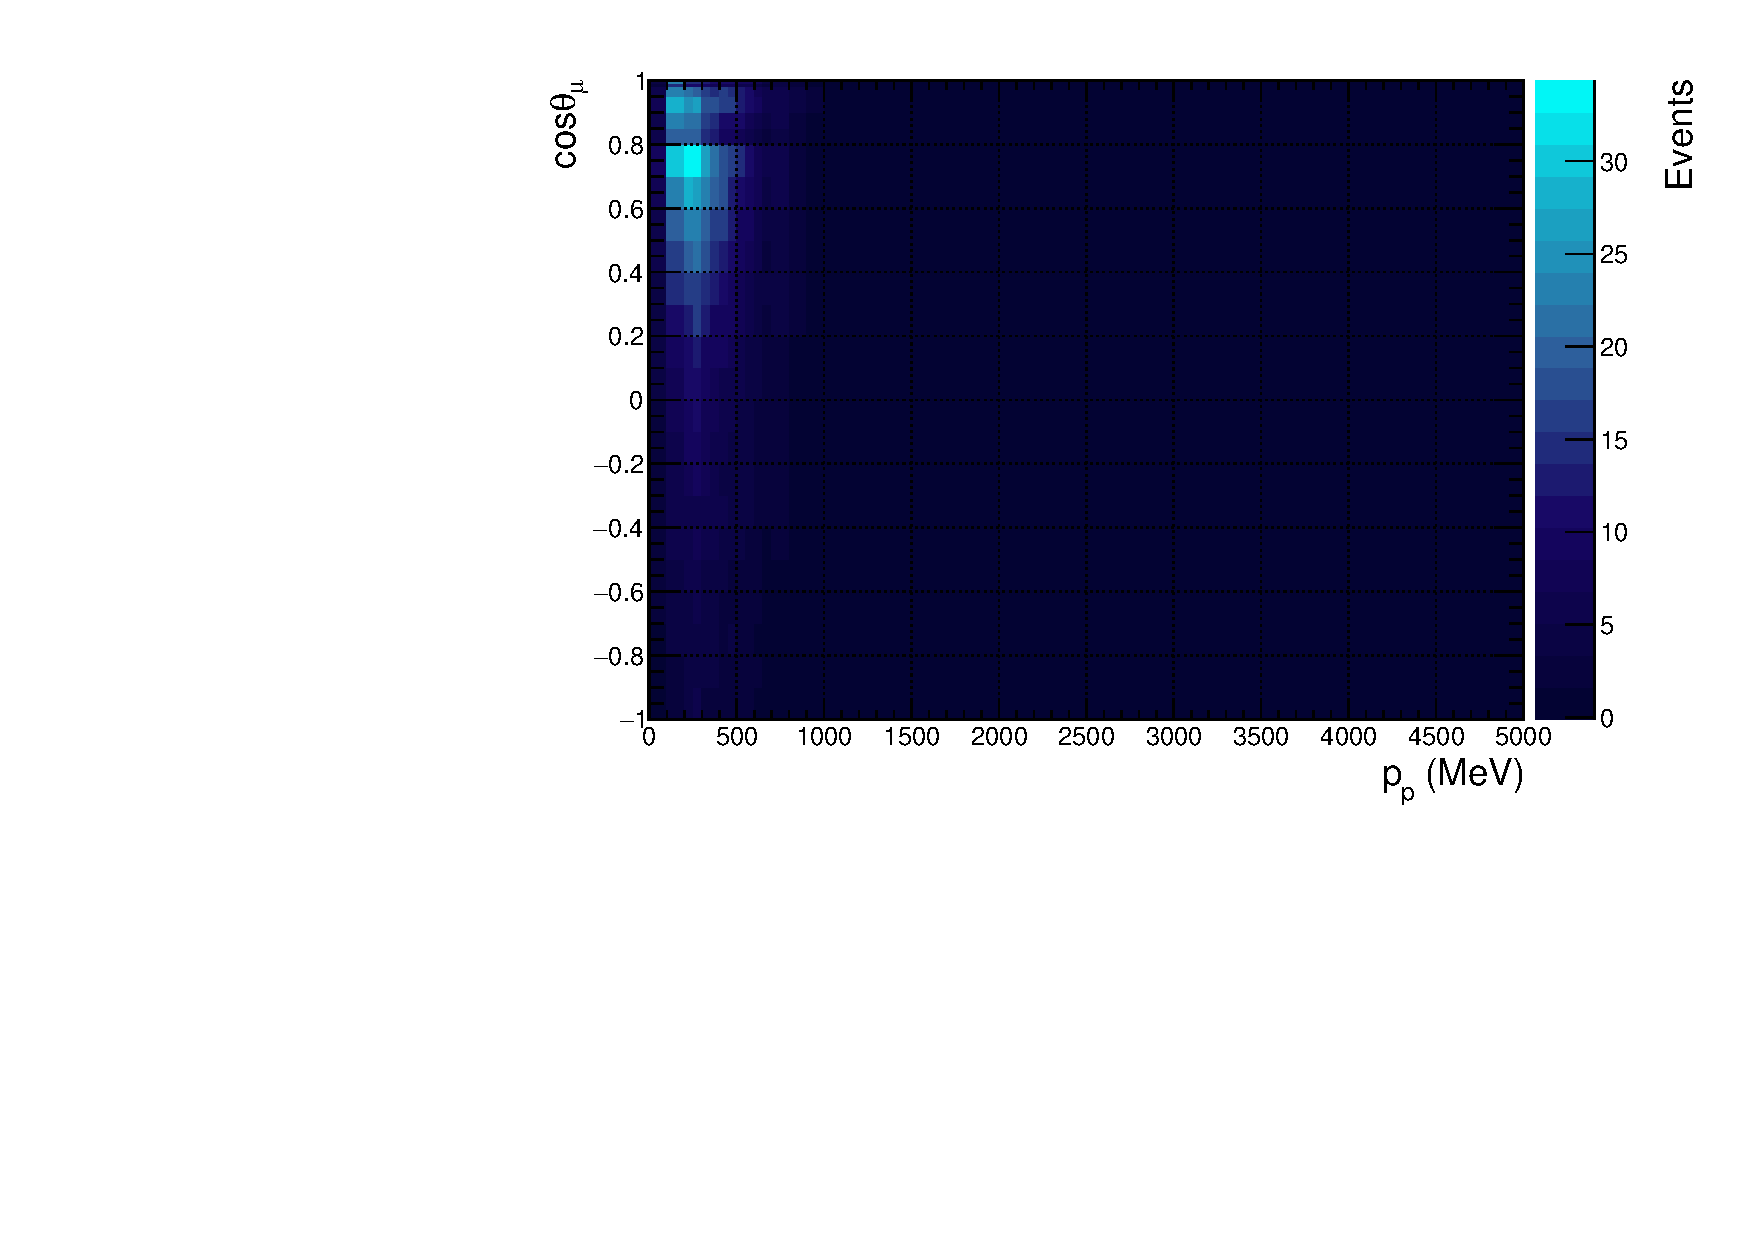
\includegraphics[width=0.9\linewidth]{figs/hptpc_sigvar_cc0piNp.pdf}
  \caption{CC 0$\pi$ Np: $p_{p}$-cos$\theta_{\mu}$}
\end{subfigure}
\begin{subfigure}{.49\textwidth}
  \centering
  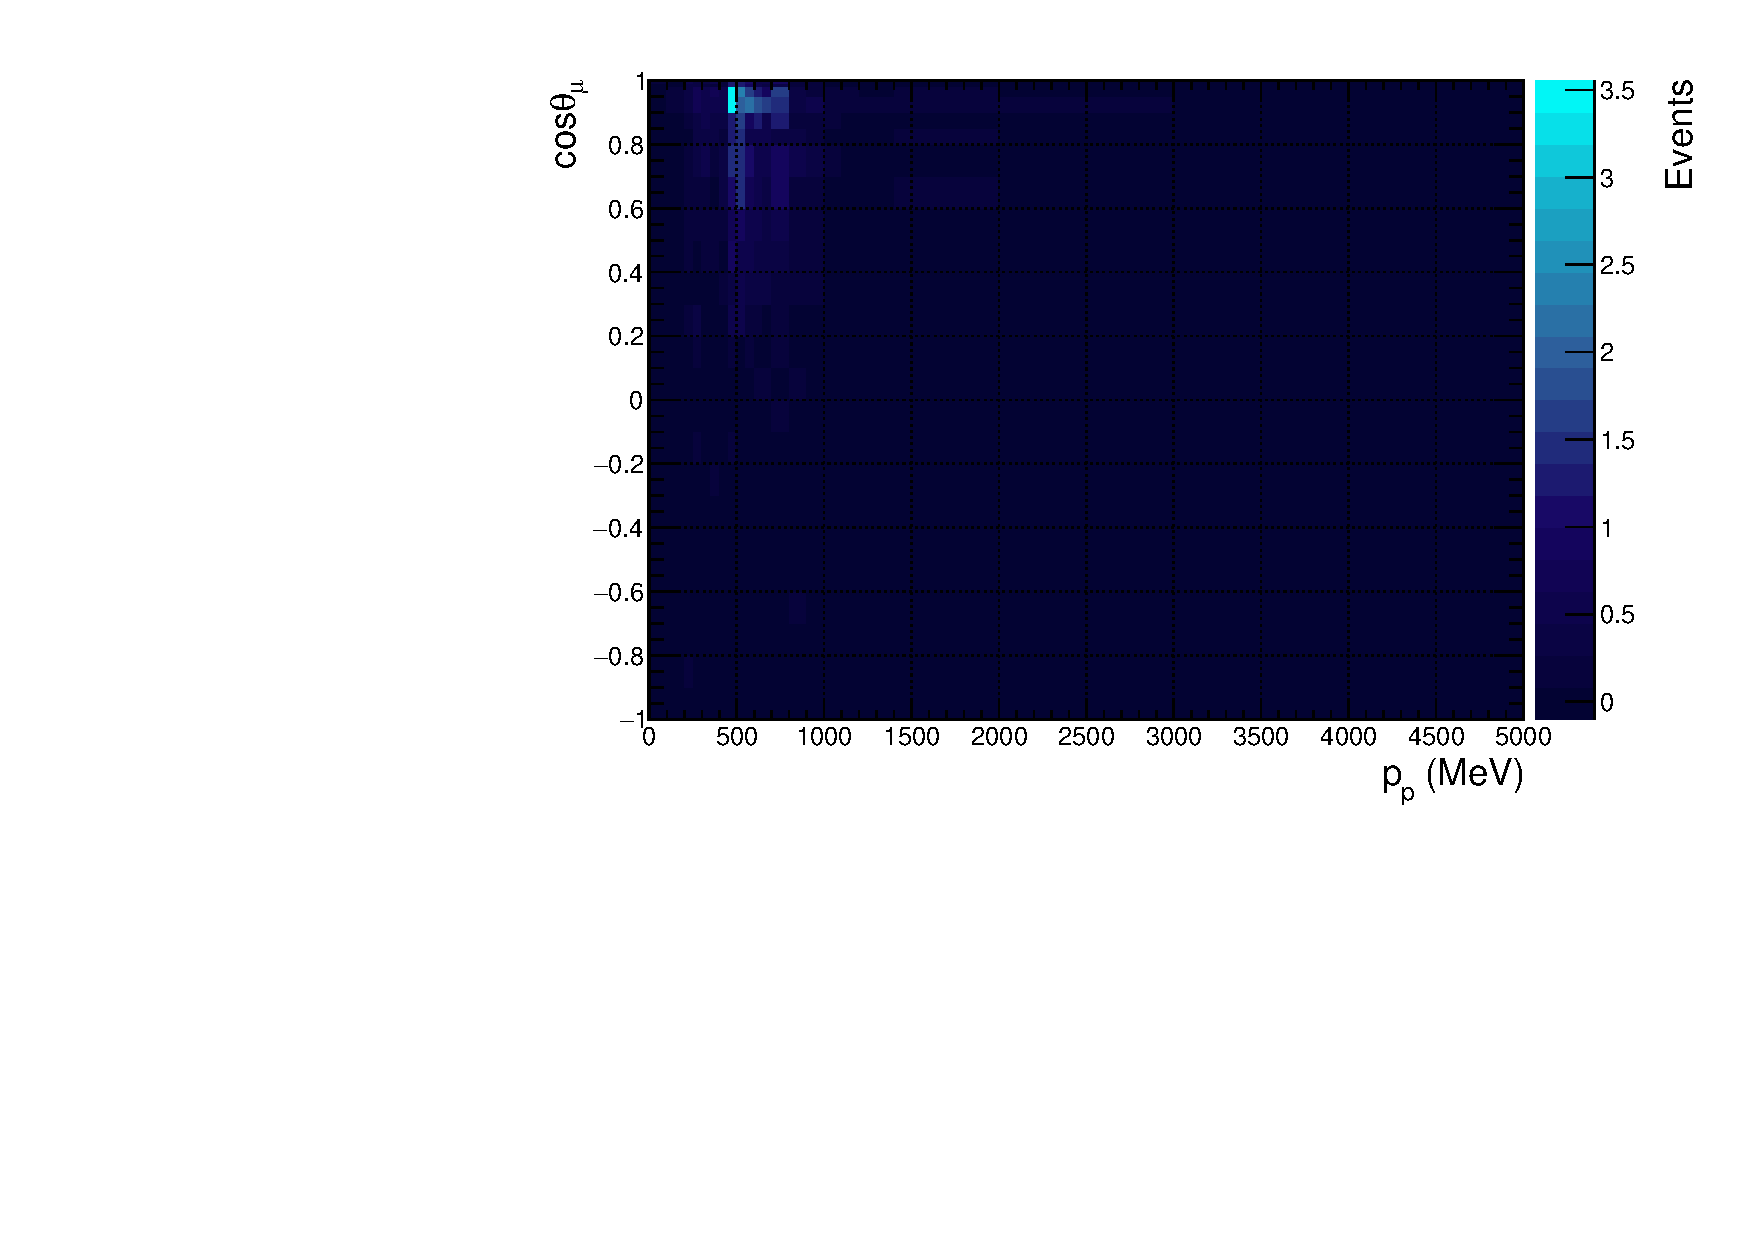
\includegraphics[width=0.9\linewidth]{figs/hptpc_sigvar_cc1piNp.pdf}
  \caption{CC 1$\pi$ Np: $p_{p}$-cos$\theta_{\mu}$}
\end{subfigure}
\begin{subfigure}{.49\textwidth}
  \centering
  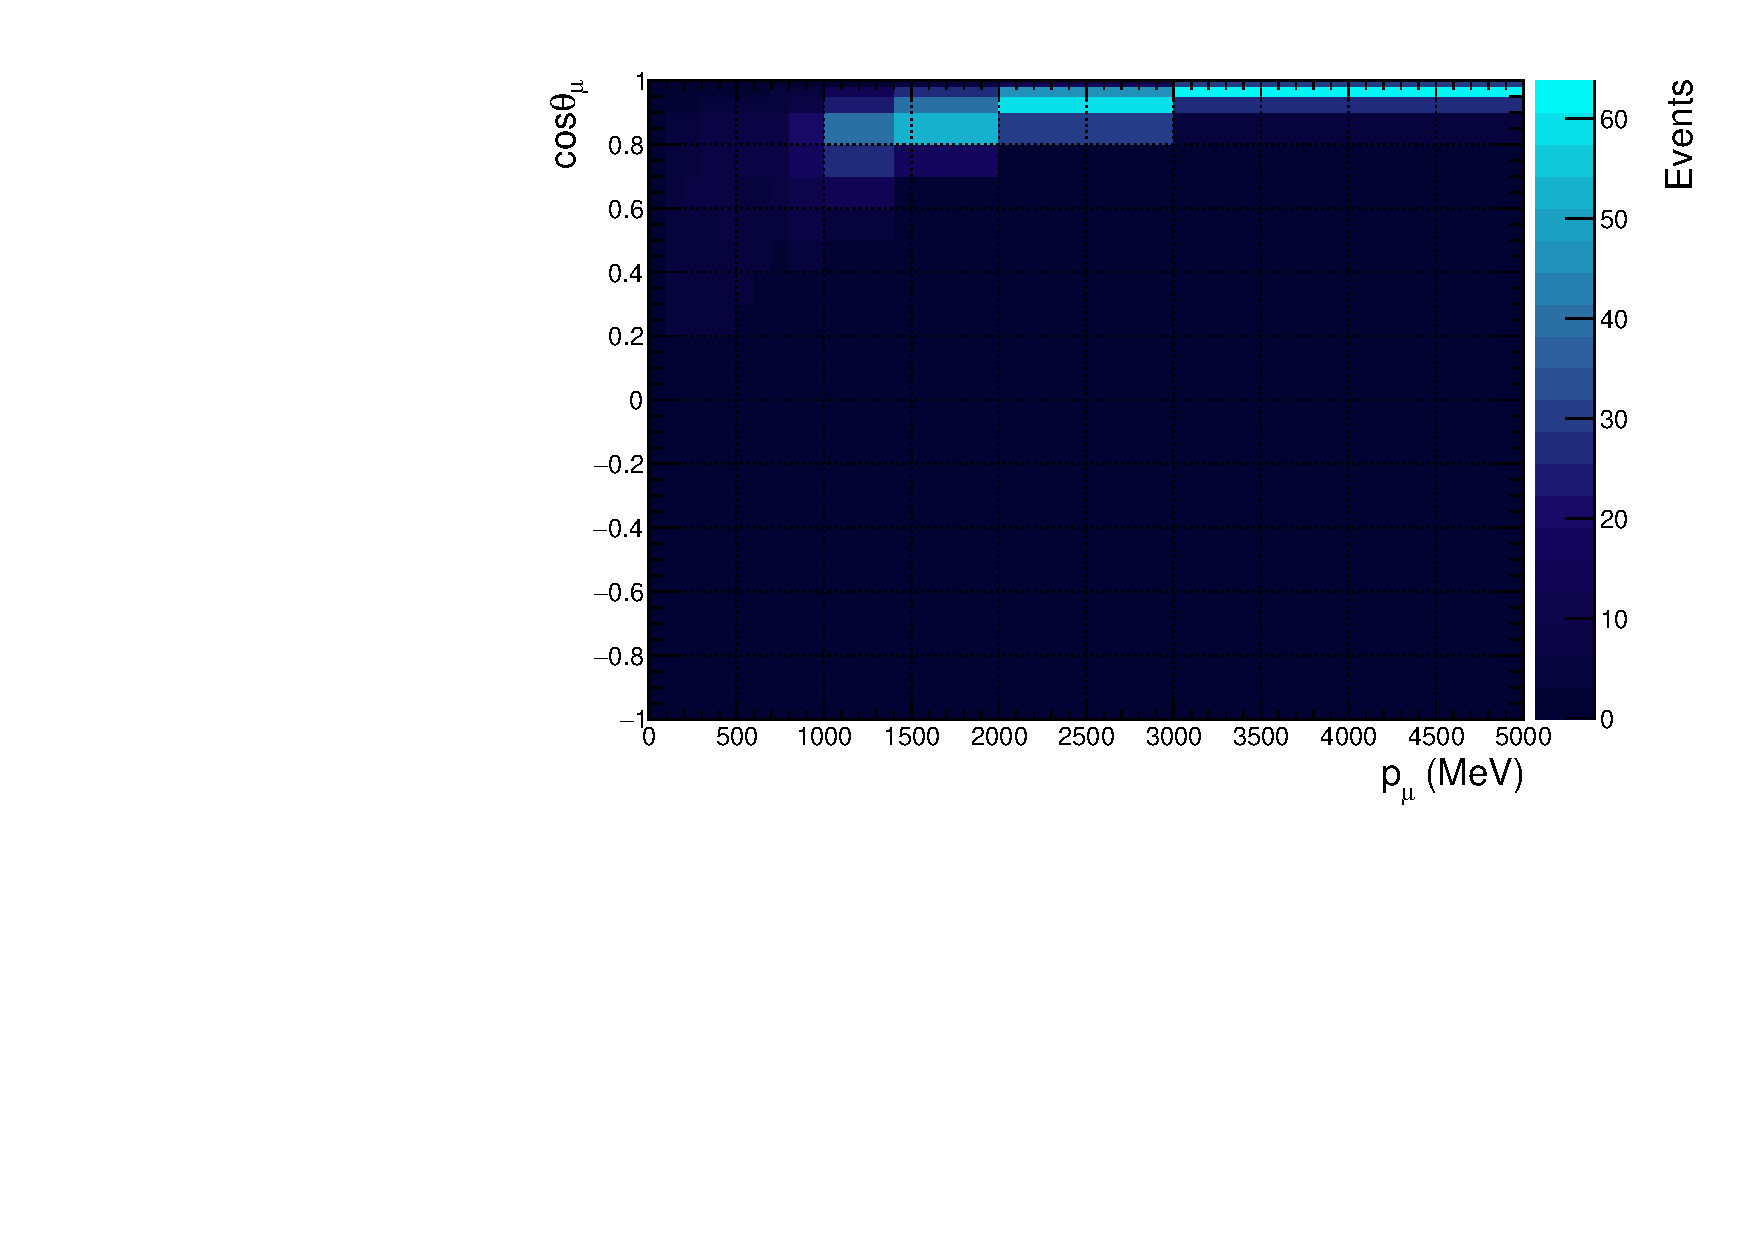
\includegraphics[width=0.9\linewidth]{figs/hptpc_sigvar_ccOther.pdf}
  \caption{CC Other: $p_{\mu}$-cos$\theta_{\mu}$}
\end{subfigure}
\caption{Distributions of HPTPC MC in different kinematic variables. For each sample, the pair of kinematics shown are those that had the largest change in event rates in $\pm1\sigma$ parameter variations.}
\label{fig:hptpcsigvar}
\end{figure}

The samples binned in $p_{p}$ and $p_{\pi}$ have hard cuts at low momentum, beyond which there are very few events. However, these are significantly below the ND280 detection thresholds. These samples, along with the $\delta p_{T}$ binned CC 1$\pi$ 1p  sample, have much narrower momentum distributions than those binned in $p_{\mu}$. The `gaps' in the distributions at cos$\theta_{\mu}\sim$0.8 are binning effects, whereby bins in the peak regions are finer, so have fewer events. The binnings have not been fully tuned to the new kinematic variables. 

\subsubsection{Asimov Fits}

Three Asimov fits were ran to compare the sensitivities of the two detectors. The ND280 and HPTPC nominal MC distributions were fit in $p_{\mu}$-cos$\theta_{\mu}$, and the HPTPC MC was also fit in the combination of single transverse variables for each sample shown in Figure \ref{fig:hptpcsigvar}.

The fit results are shown in Figures \ref{fig:hptpcfluxND}, \ref{fig:hptpcfluxSK} and \ref{fig:hptpcxsec}.

\begin{figure}
\centering
\begin{subfigure}{0.3\textwidth}
  \centering
  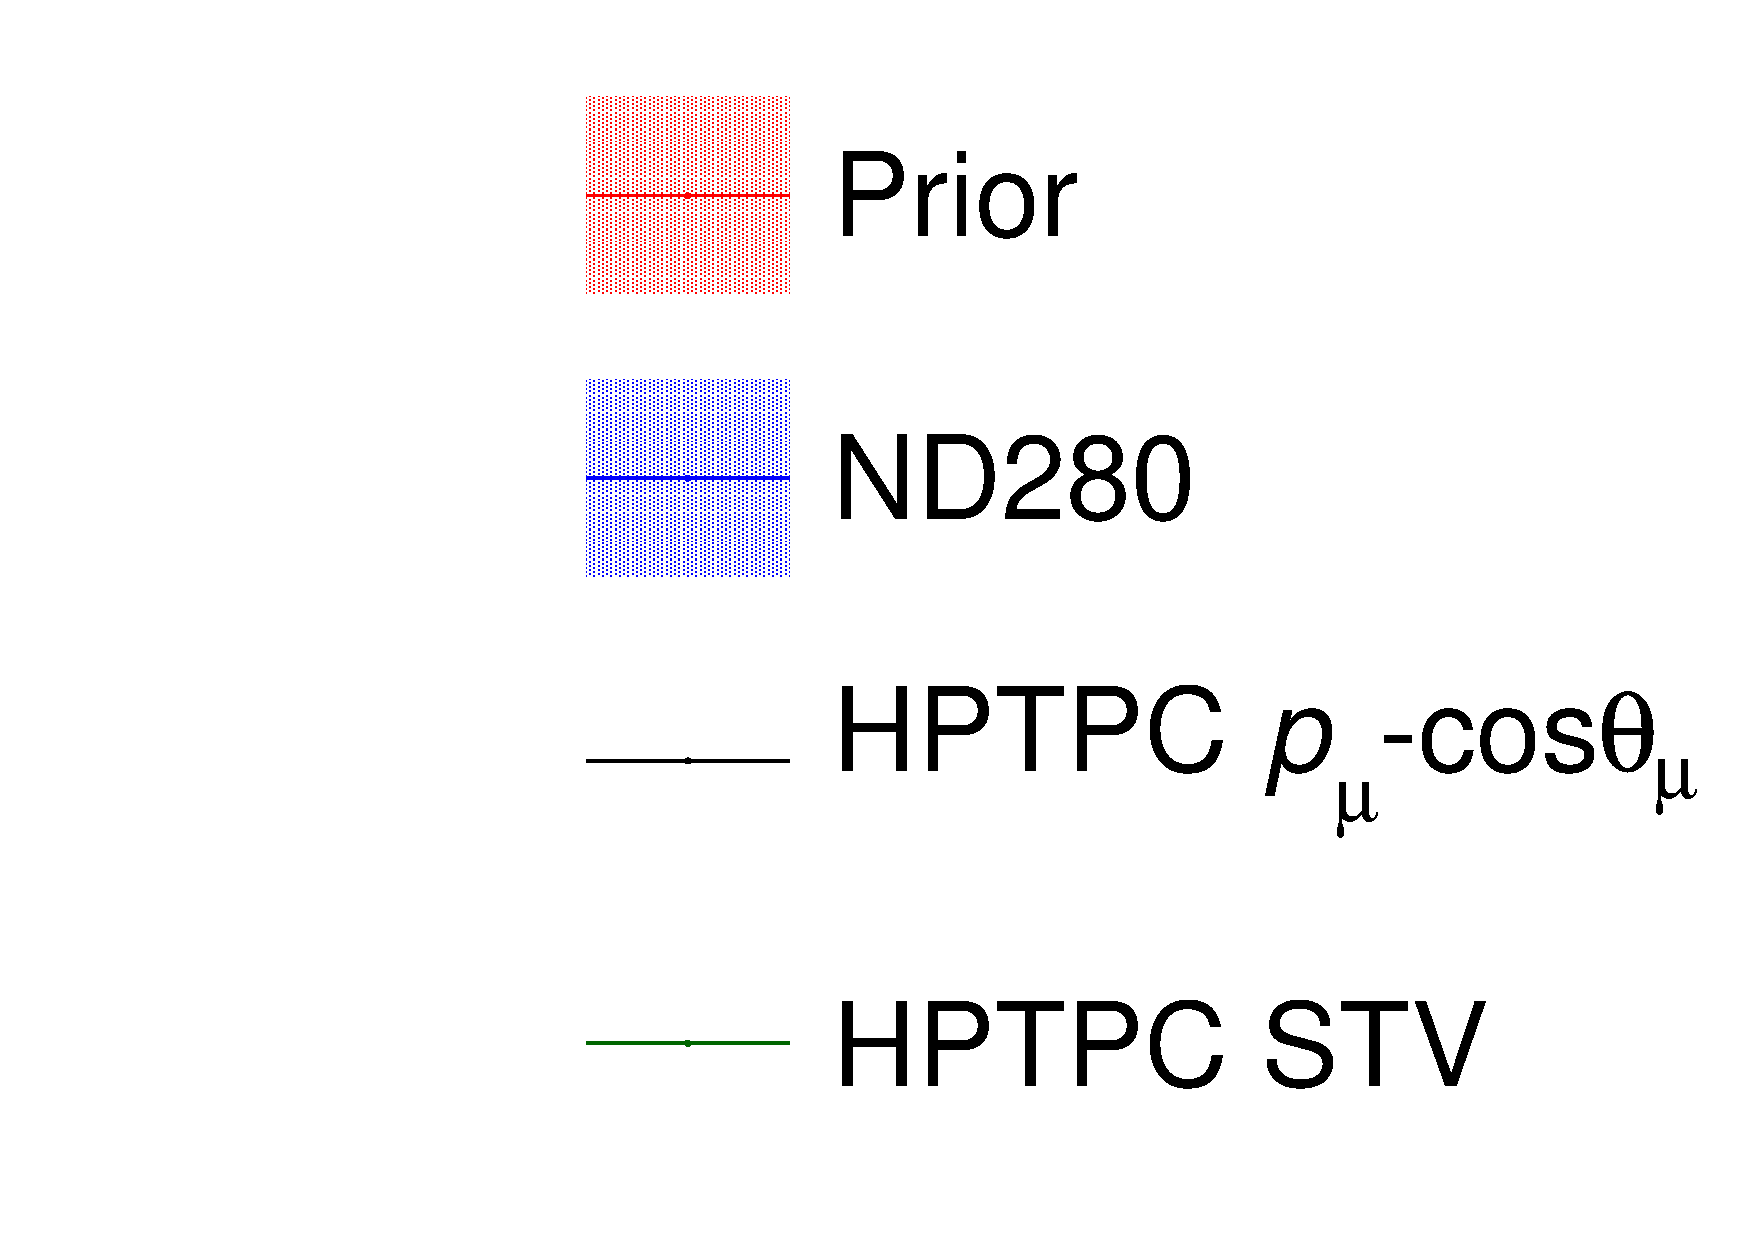
\includegraphics[width=1.0\linewidth, trim={5mm  90mm 0mm 0mm}, clip]{figs/hptpcfits_leg}	
\end{subfigure}
\begin{subfigure}{0.3\textwidth}
  \centering
  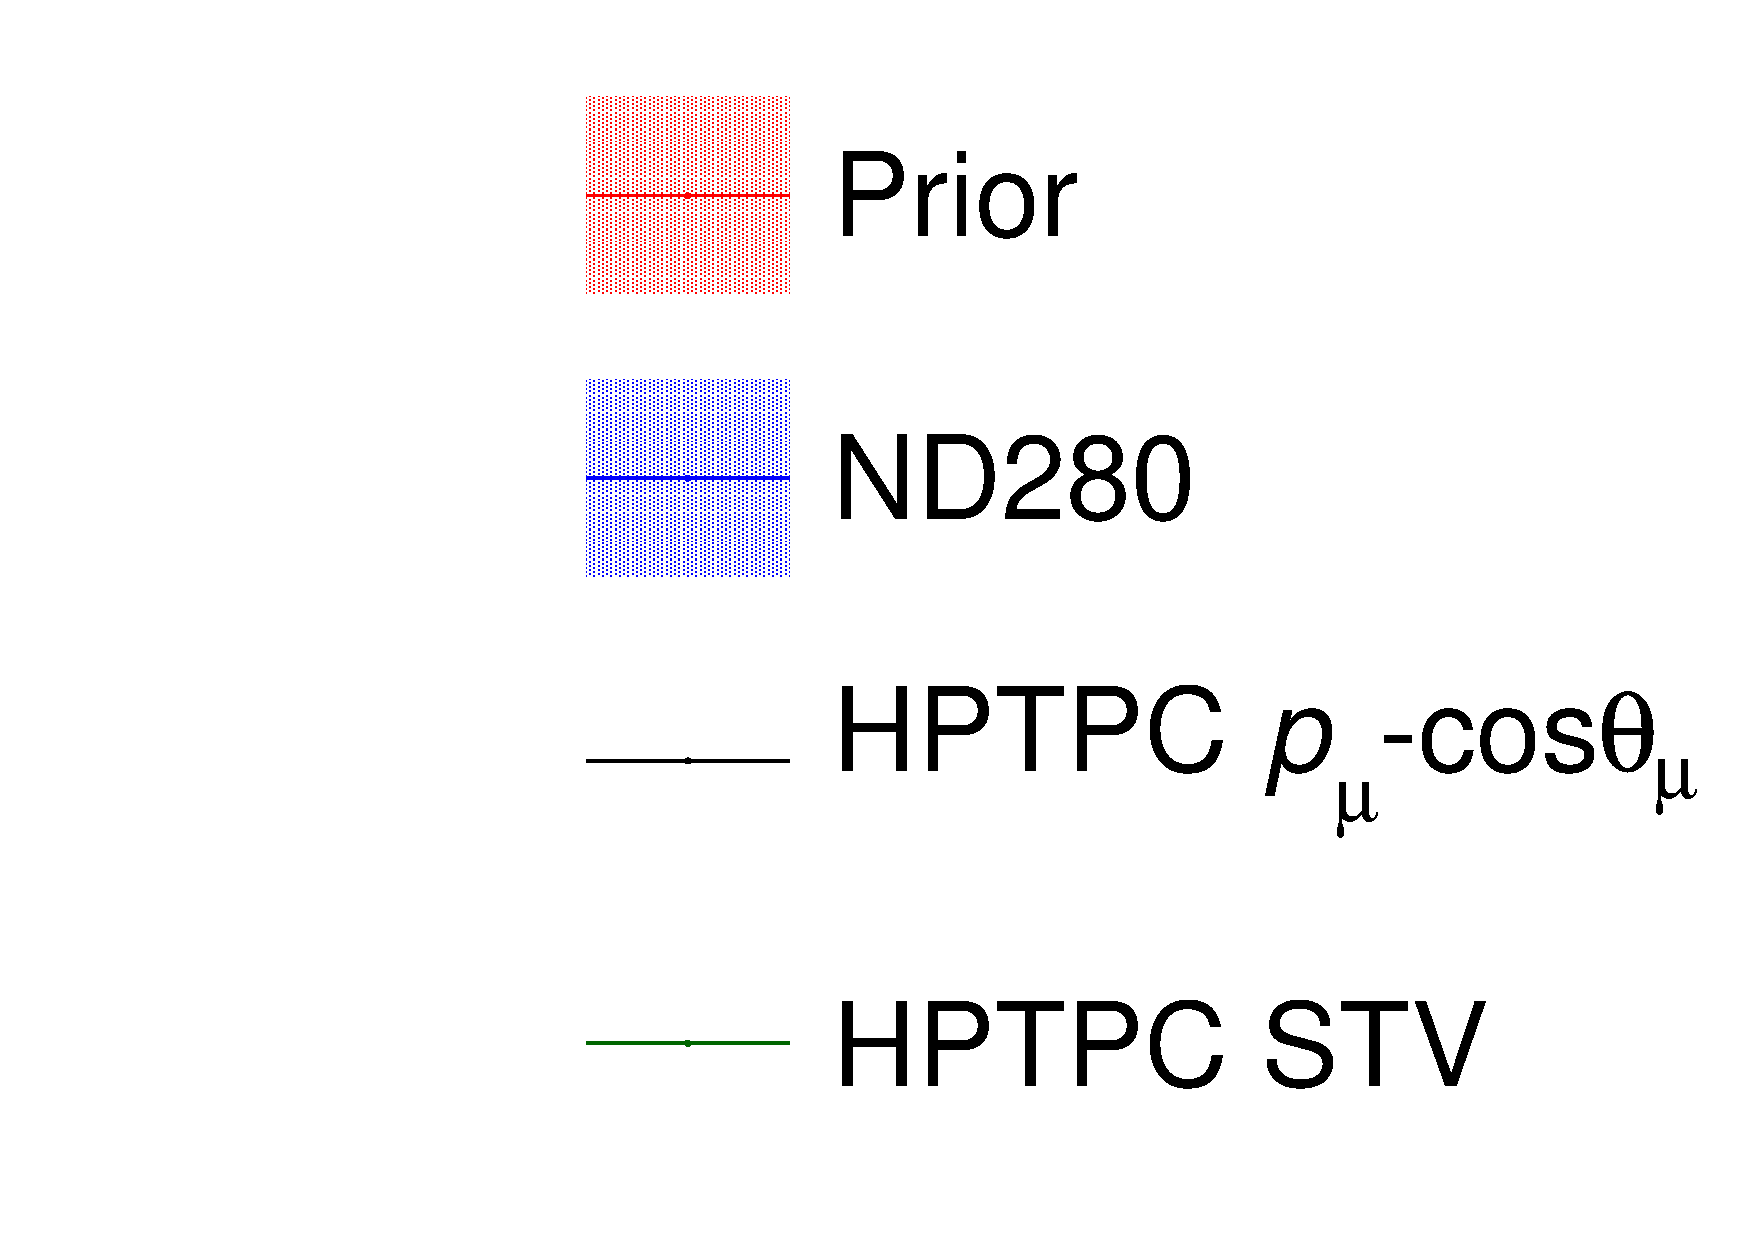
\includegraphics[width=1.0\linewidth, trim={5mm  0mm 0mm 95mm}, clip]{figs/hptpcfits_leg}	
\end{subfigure}
\begin{subfigure}{0.45\textwidth}
  \centering
  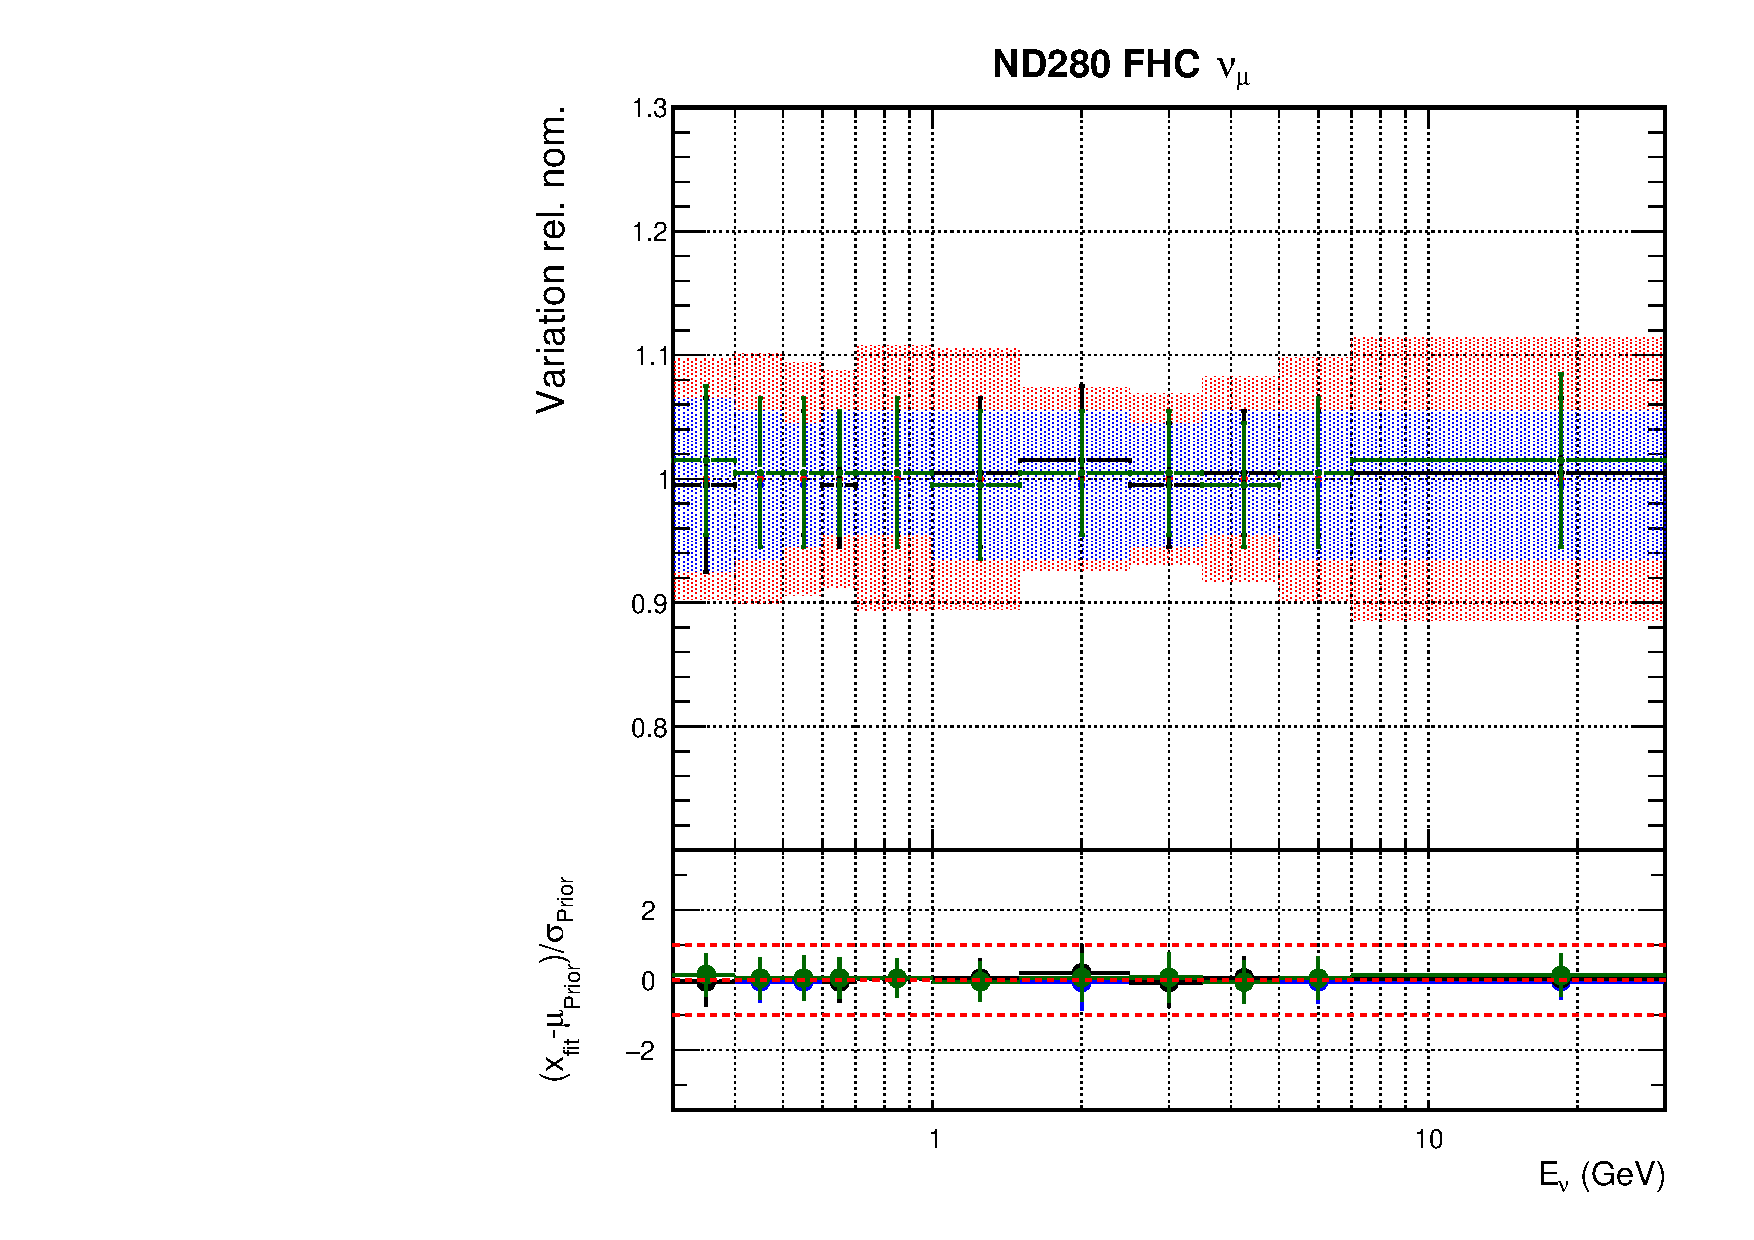
\includegraphics[width=0.75\linewidth]{figs/hptpcfitsflux_0}
  \caption{ND FHC $\nu_{\mu}$}
\end{subfigure}
\begin{subfigure}{0.45\textwidth}
  \centering
  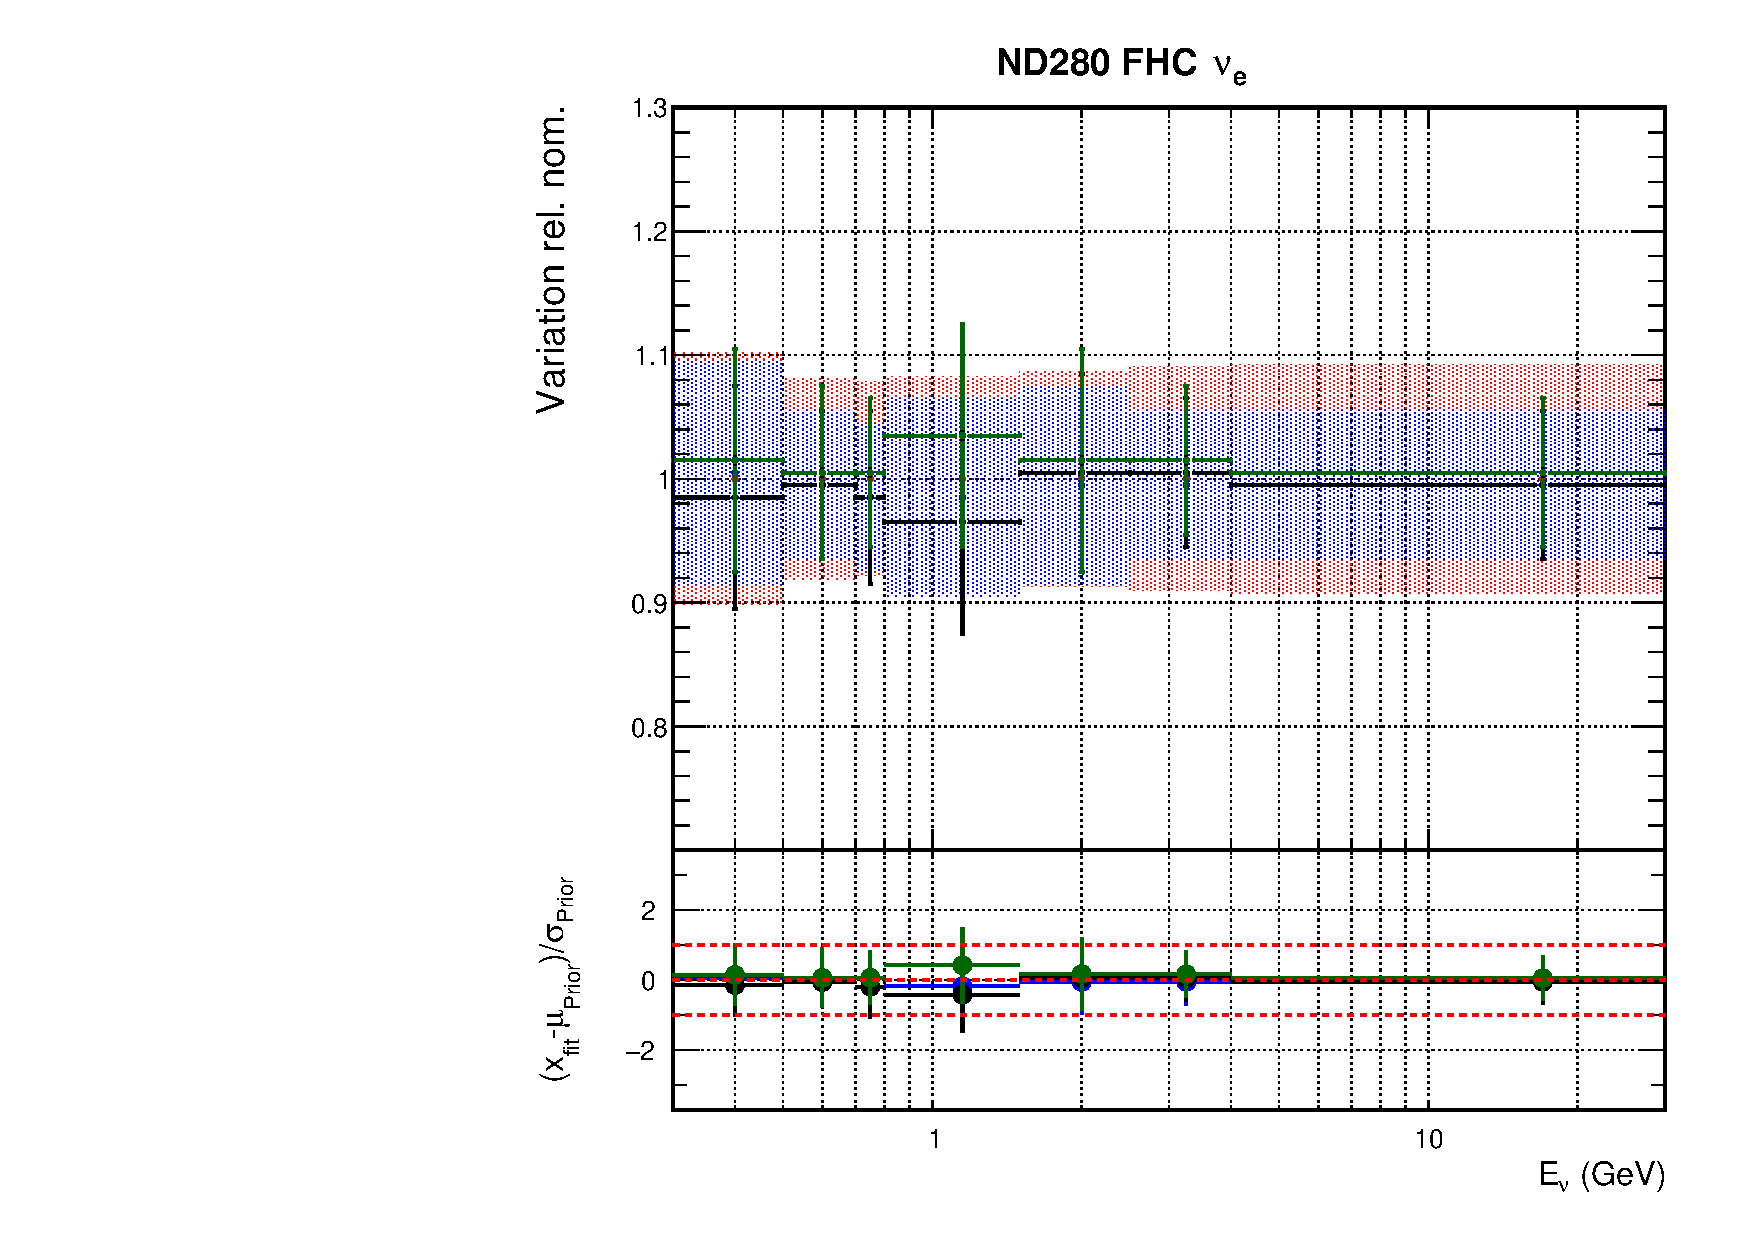
\includegraphics[width=0.75\linewidth]{figs/hptpcfitsflux_1}
  \caption{ND FHC $\bar{\nu_{\mu}}$}
\end{subfigure}
\begin{subfigure}{0.45\textwidth}
  \centering
  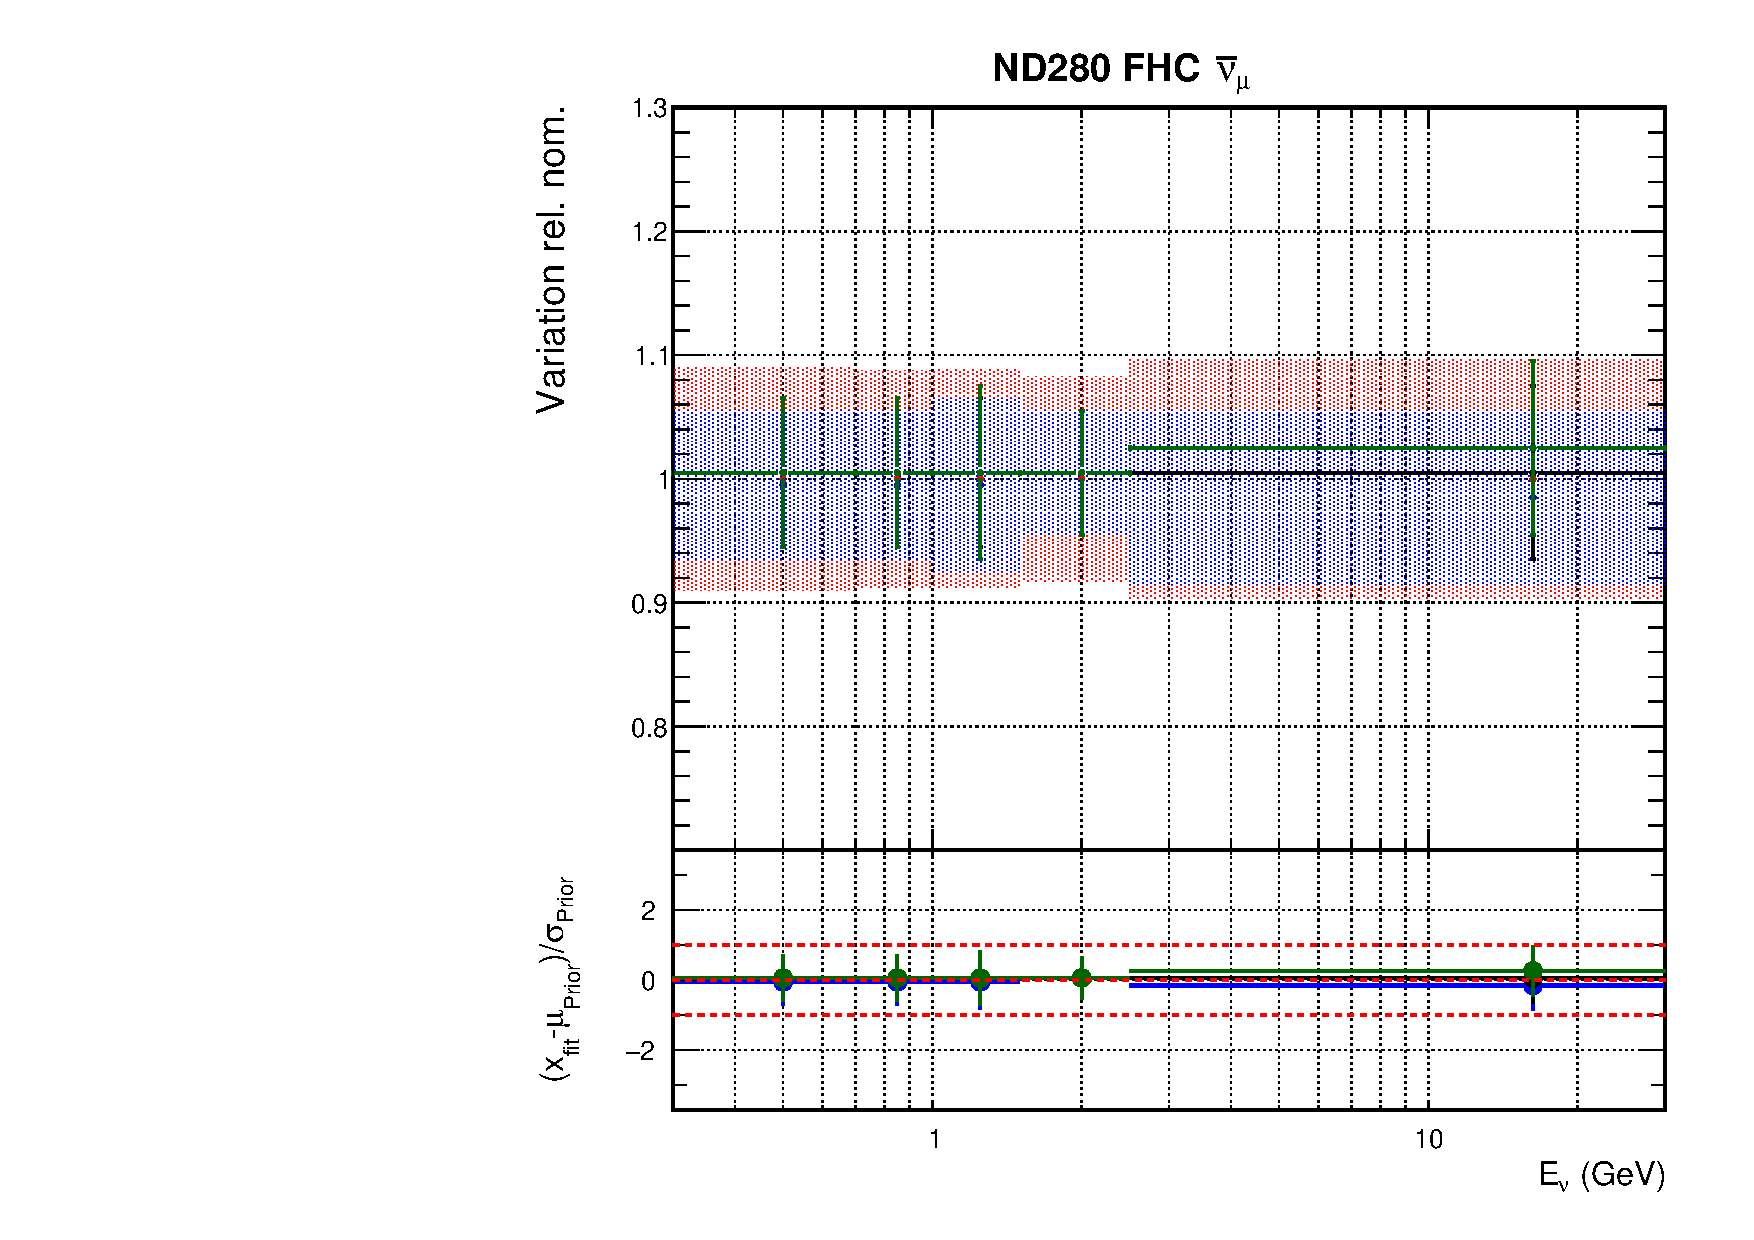
\includegraphics[width=0.75\linewidth]{figs/hptpcfitsflux_2}
  \caption{ND FHC $\nu_e$}
\end{subfigure}
\begin{subfigure}{0.45\textwidth}
  \centering
  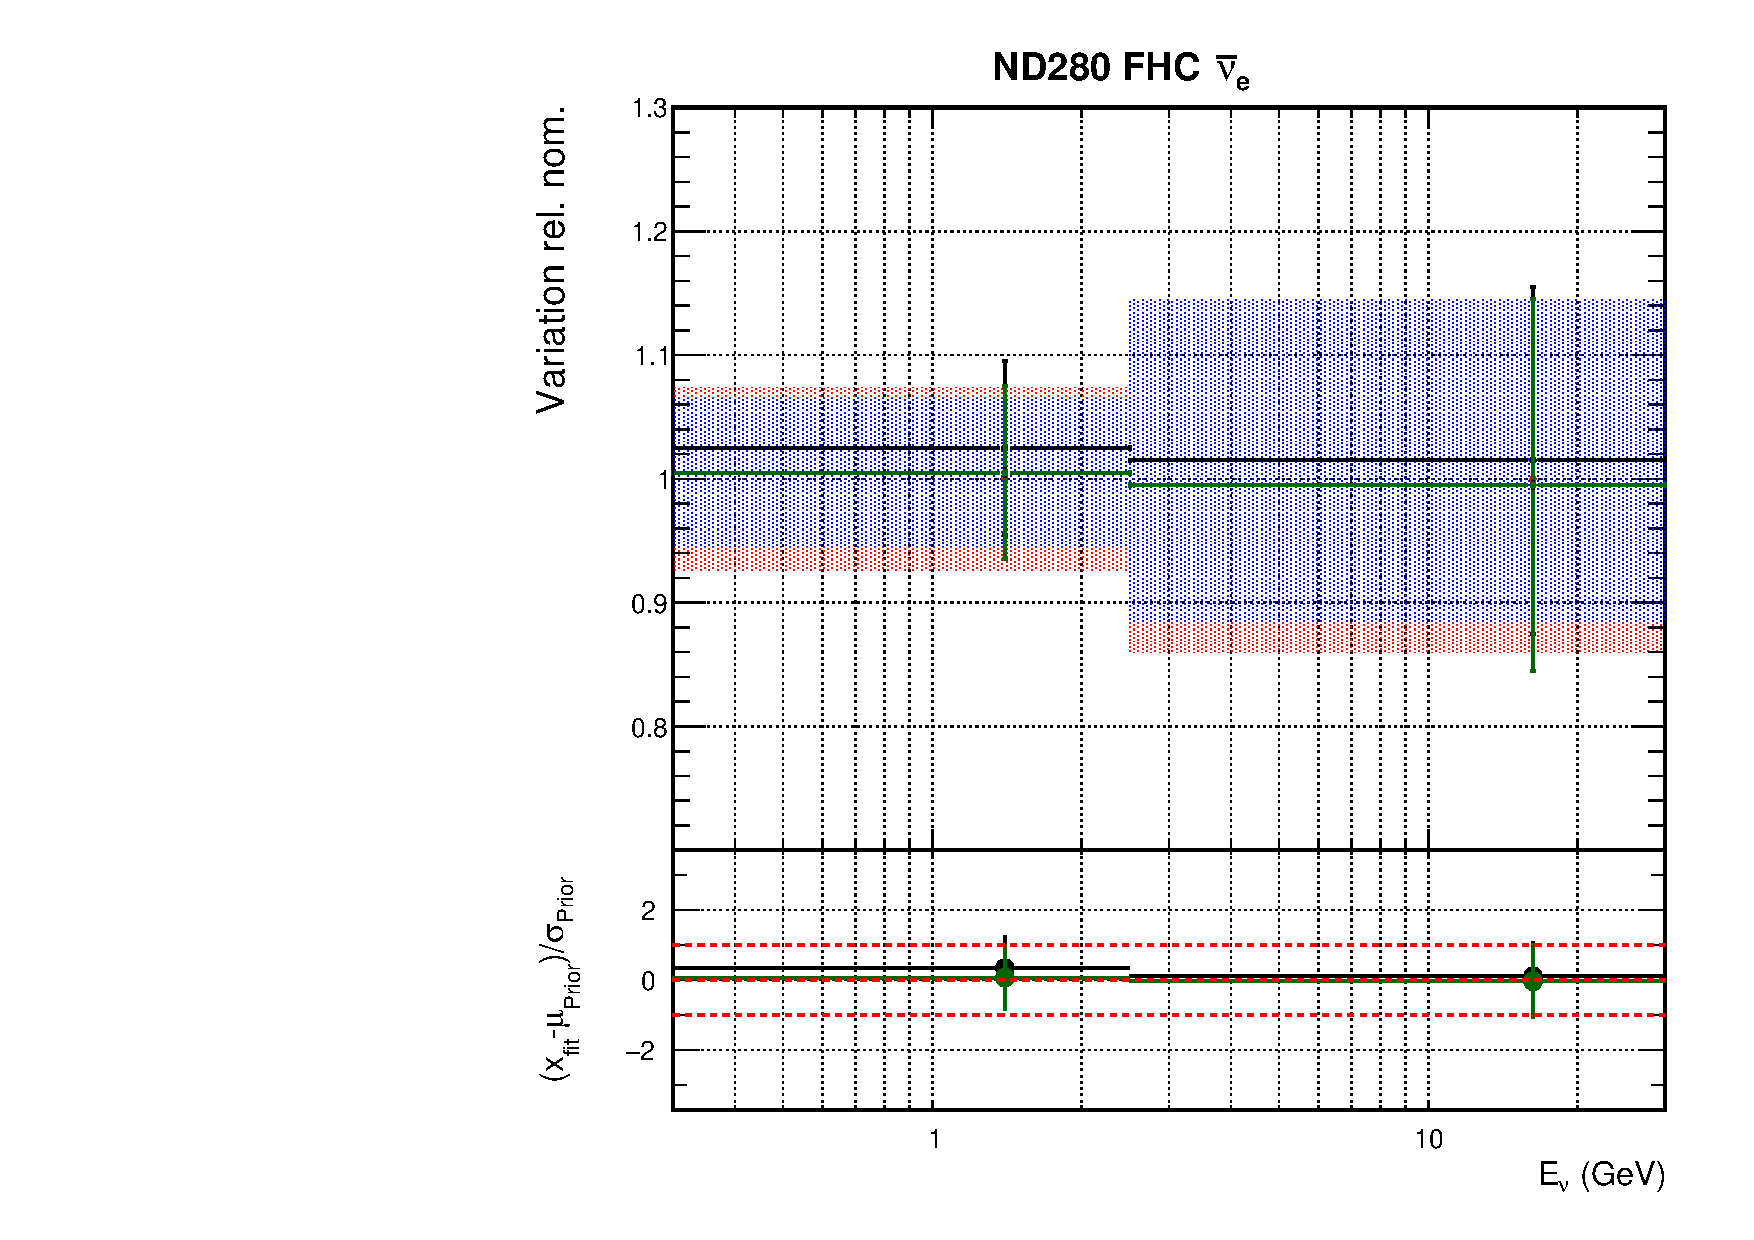
\includegraphics[width=0.75\linewidth]{figs/hptpcfitsflux_3}
  \caption{ND FHC $\bar{\nu_{e}}$}
\end{subfigure}
\begin{subfigure}{0.45\textwidth}
  \centering
  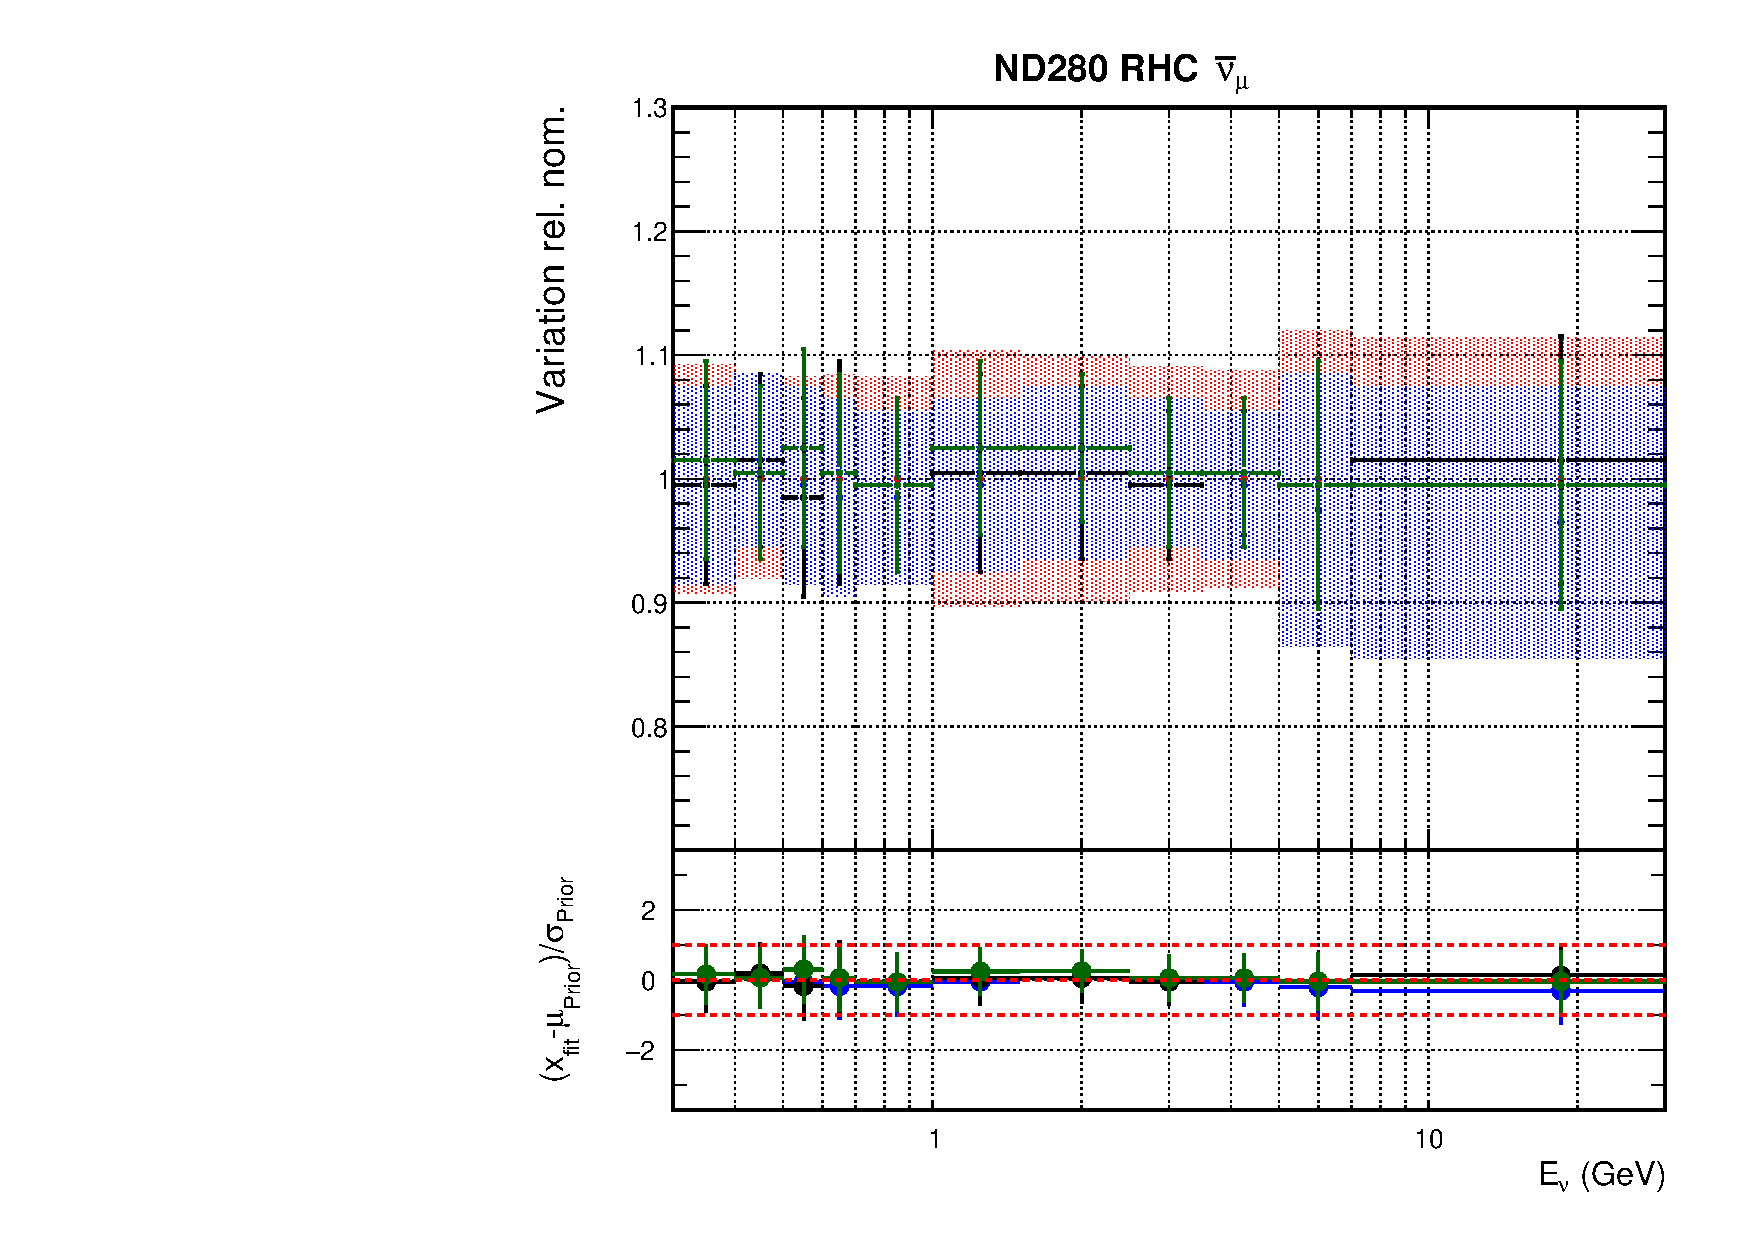
\includegraphics[width=0.75\linewidth]{figs/hptpcfitsflux_4}
  \caption{ND RHC $\nu_{\mu}$}
\end{subfigure}
\begin{subfigure}{0.45\textwidth}
  \centering
  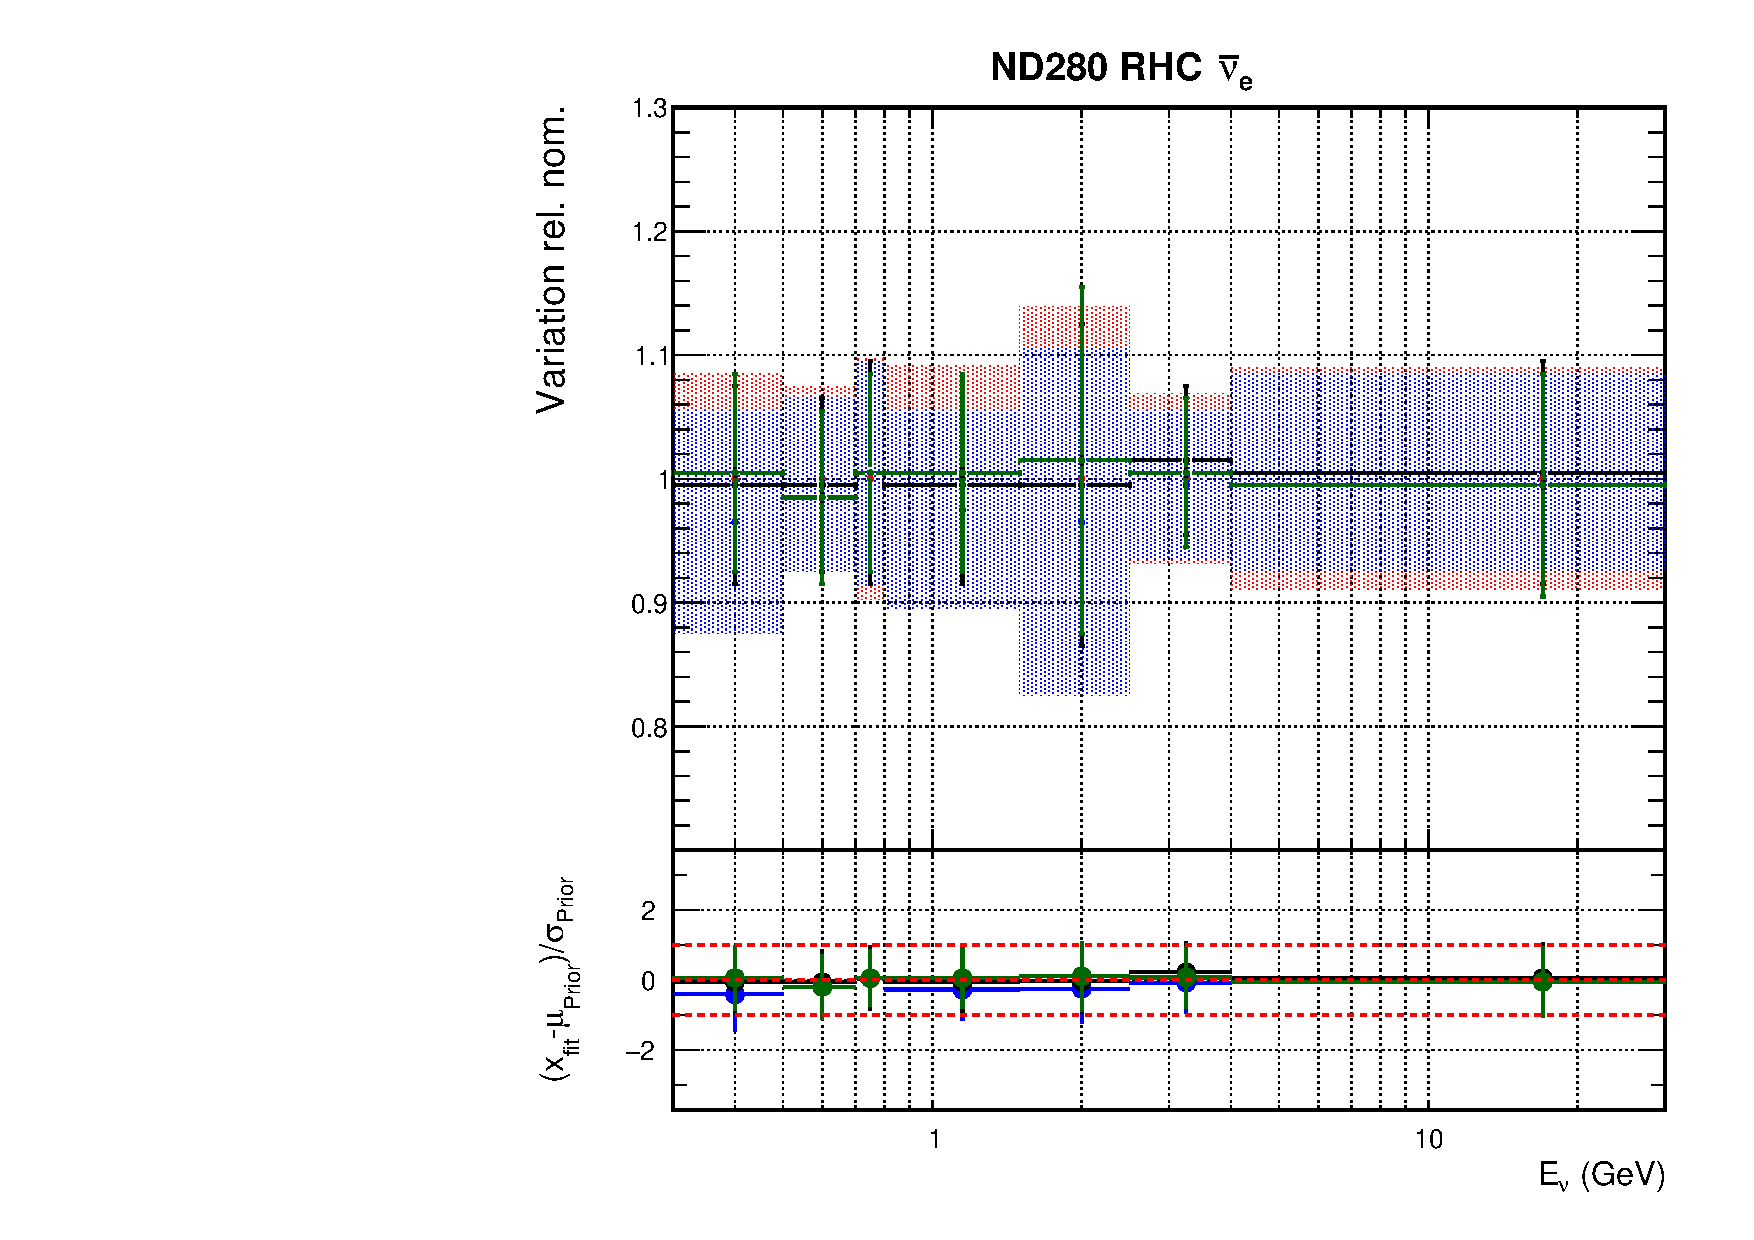
\includegraphics[width=0.75\linewidth]{figs/hptpcfitsflux_5}
  \caption{ND RHC $\bar{\nu_{\mu}}$}
\end{subfigure}
\begin{subfigure}{0.45\textwidth}
  \centering
  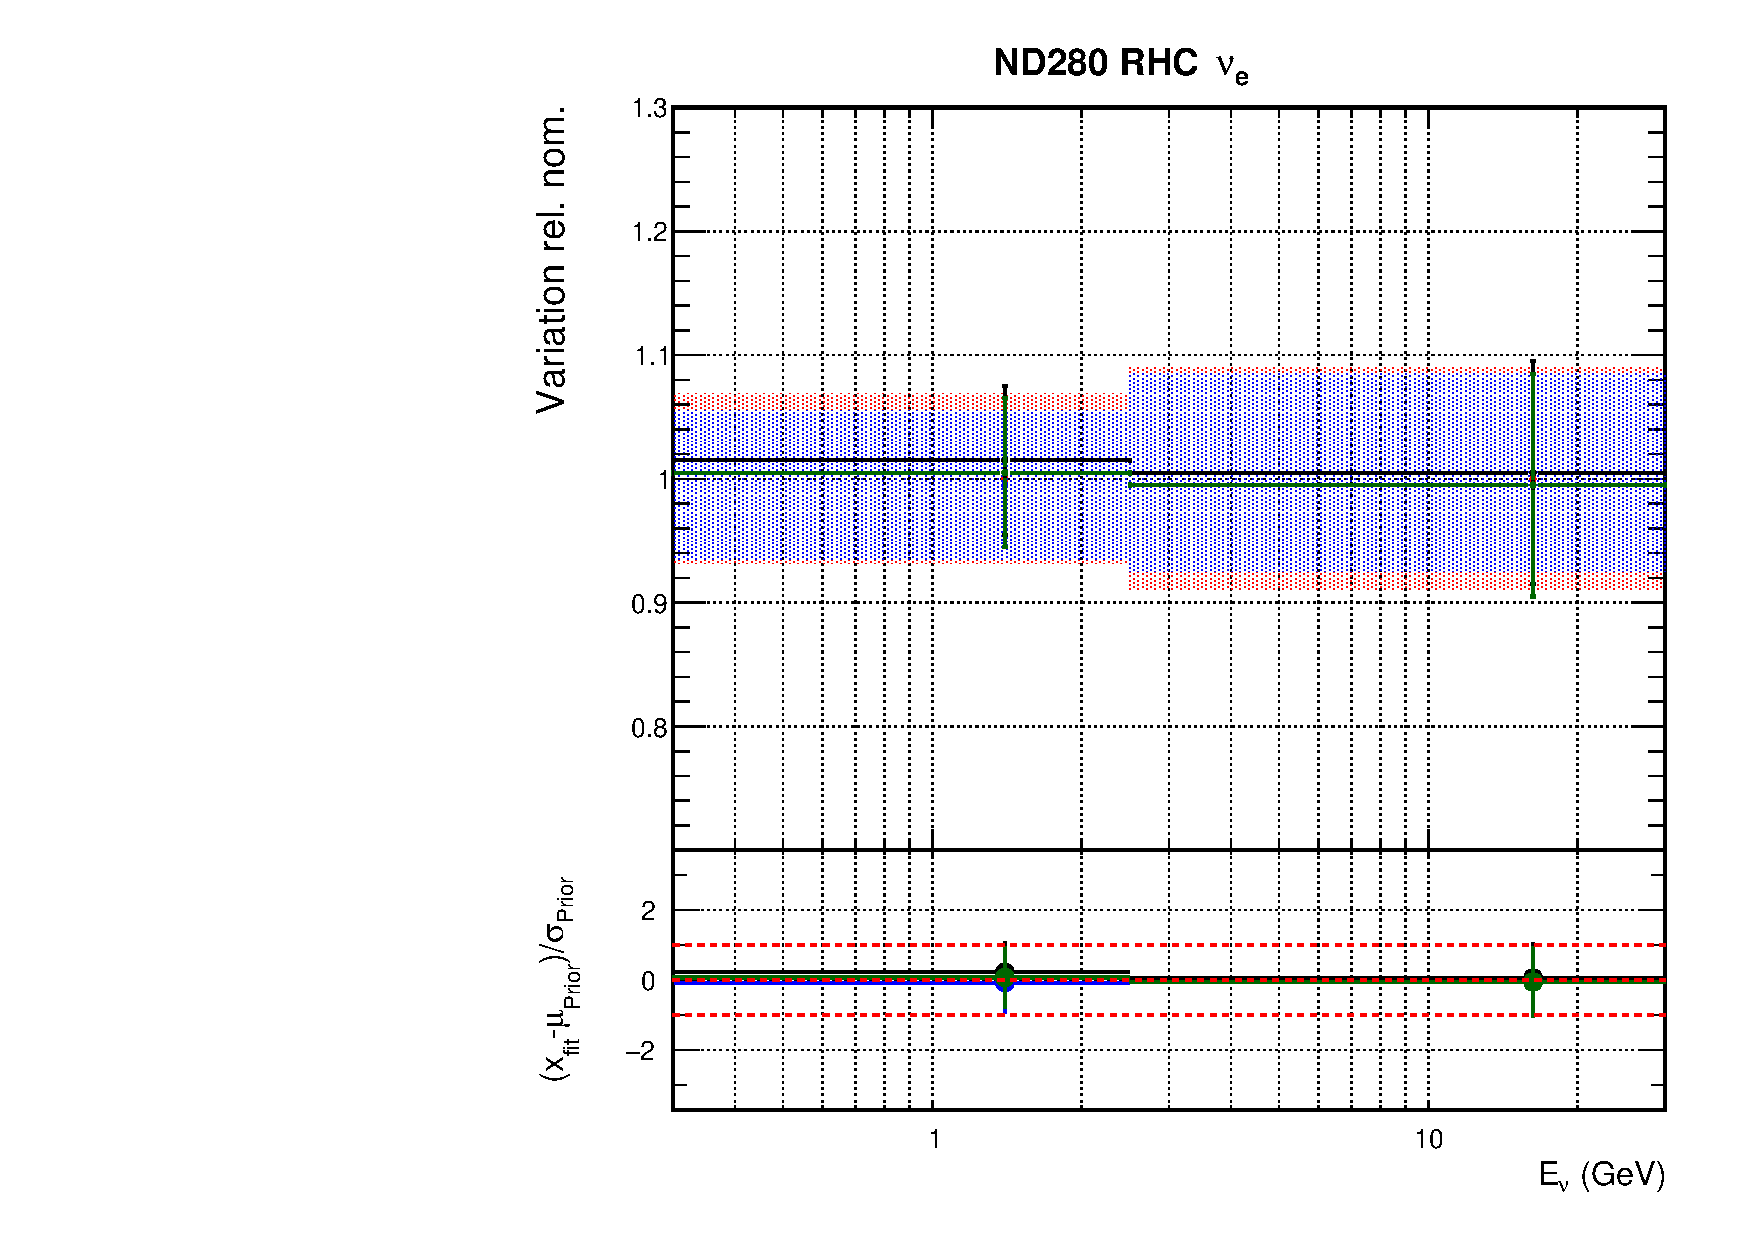
\includegraphics[width=0.75\linewidth]{figs/hptpcfitsflux_6}
  \caption{ND RHC $\nu_{e}$}
\end{subfigure}
\begin{subfigure}{0.45\textwidth}
  \centering
  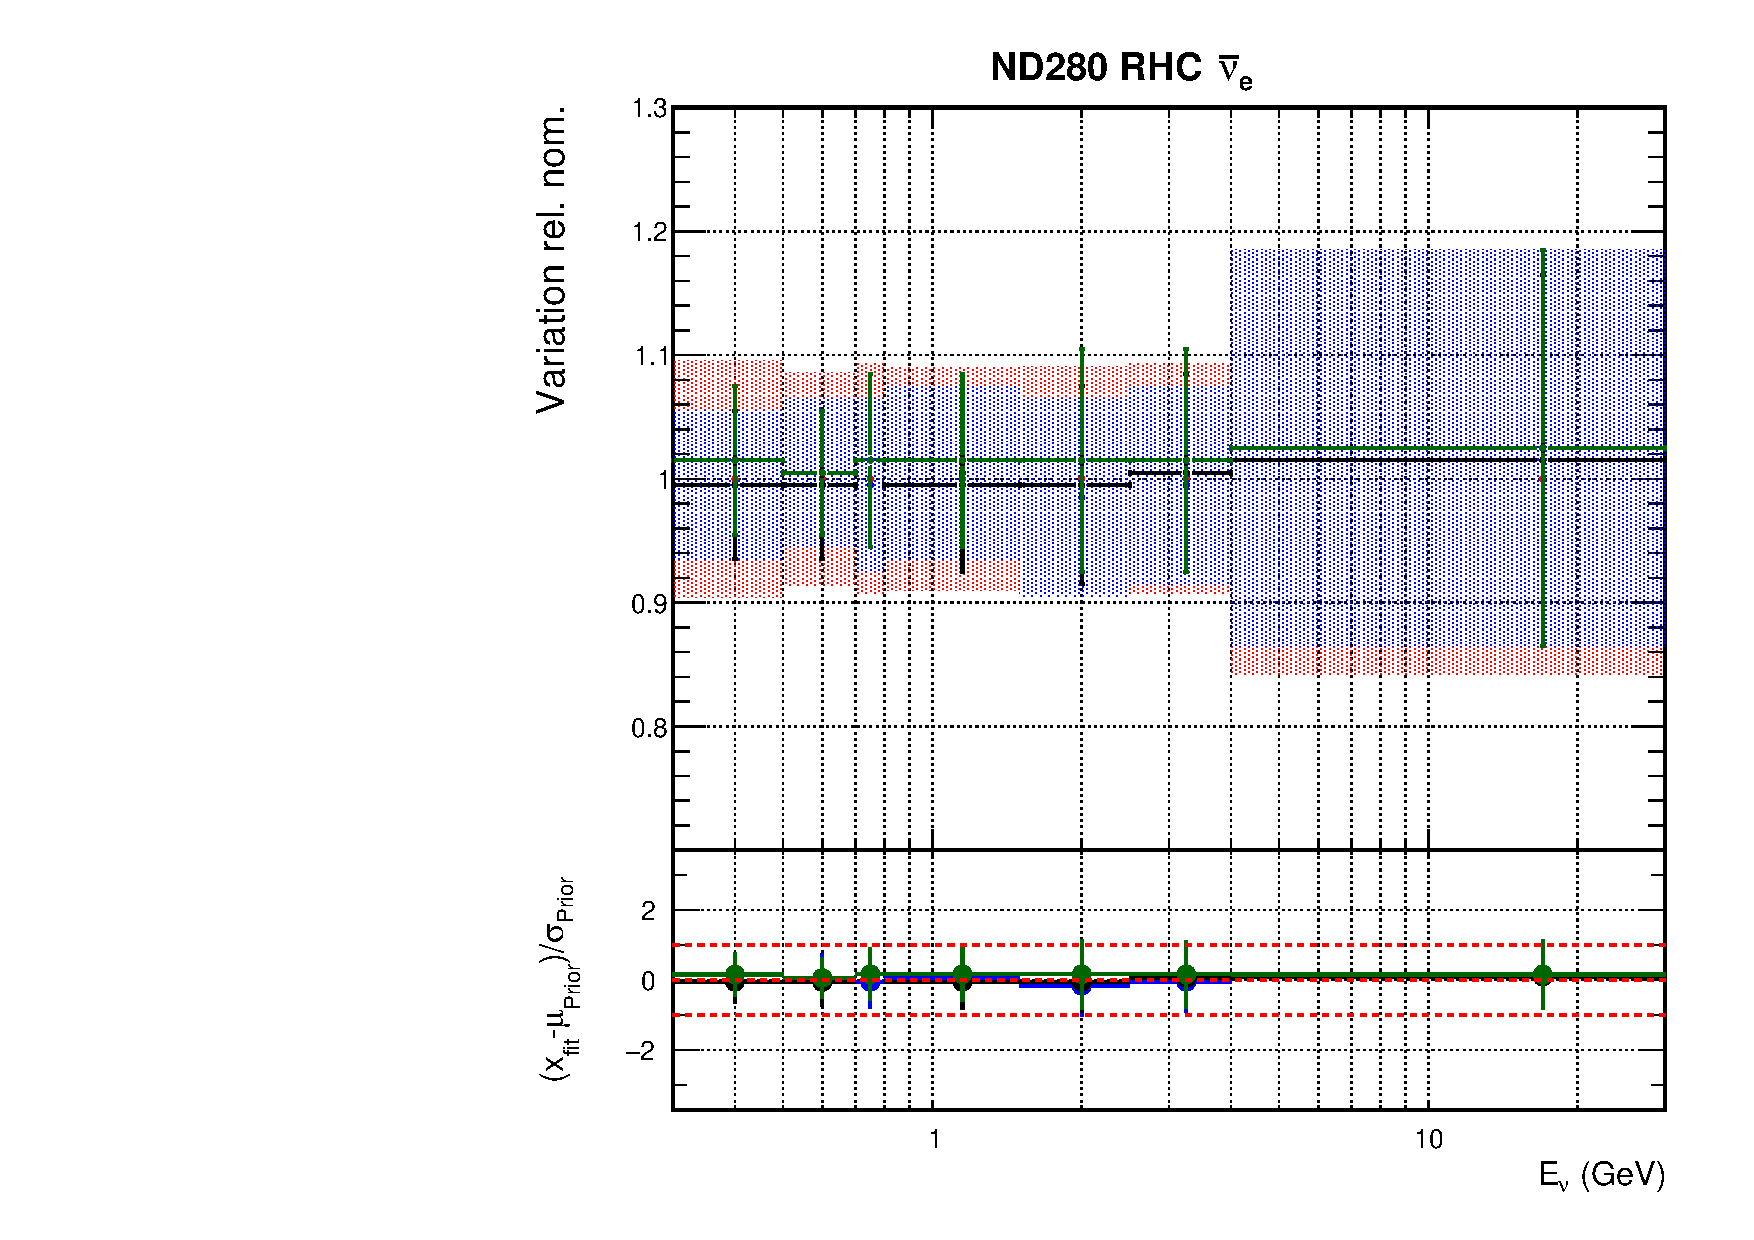
\includegraphics[width=0.75\linewidth]{figs/hptpcfitsflux_7}
  \caption{ND RHC $\bar{\nu_e}$}
\end{subfigure}
\caption{ND280 flux parameters for ND280 $p_{\mu}$-cos$\theta_{\mu}$, HPTPC $p_{\mu}$-cos$\theta_{\mu}$, and HPTPC mixed STV fits.}
\label{fig:hptpcfluxND}
\end{figure}

\begin{figure}
\centering
\begin{subfigure}{0.3\textwidth}
  \centering
  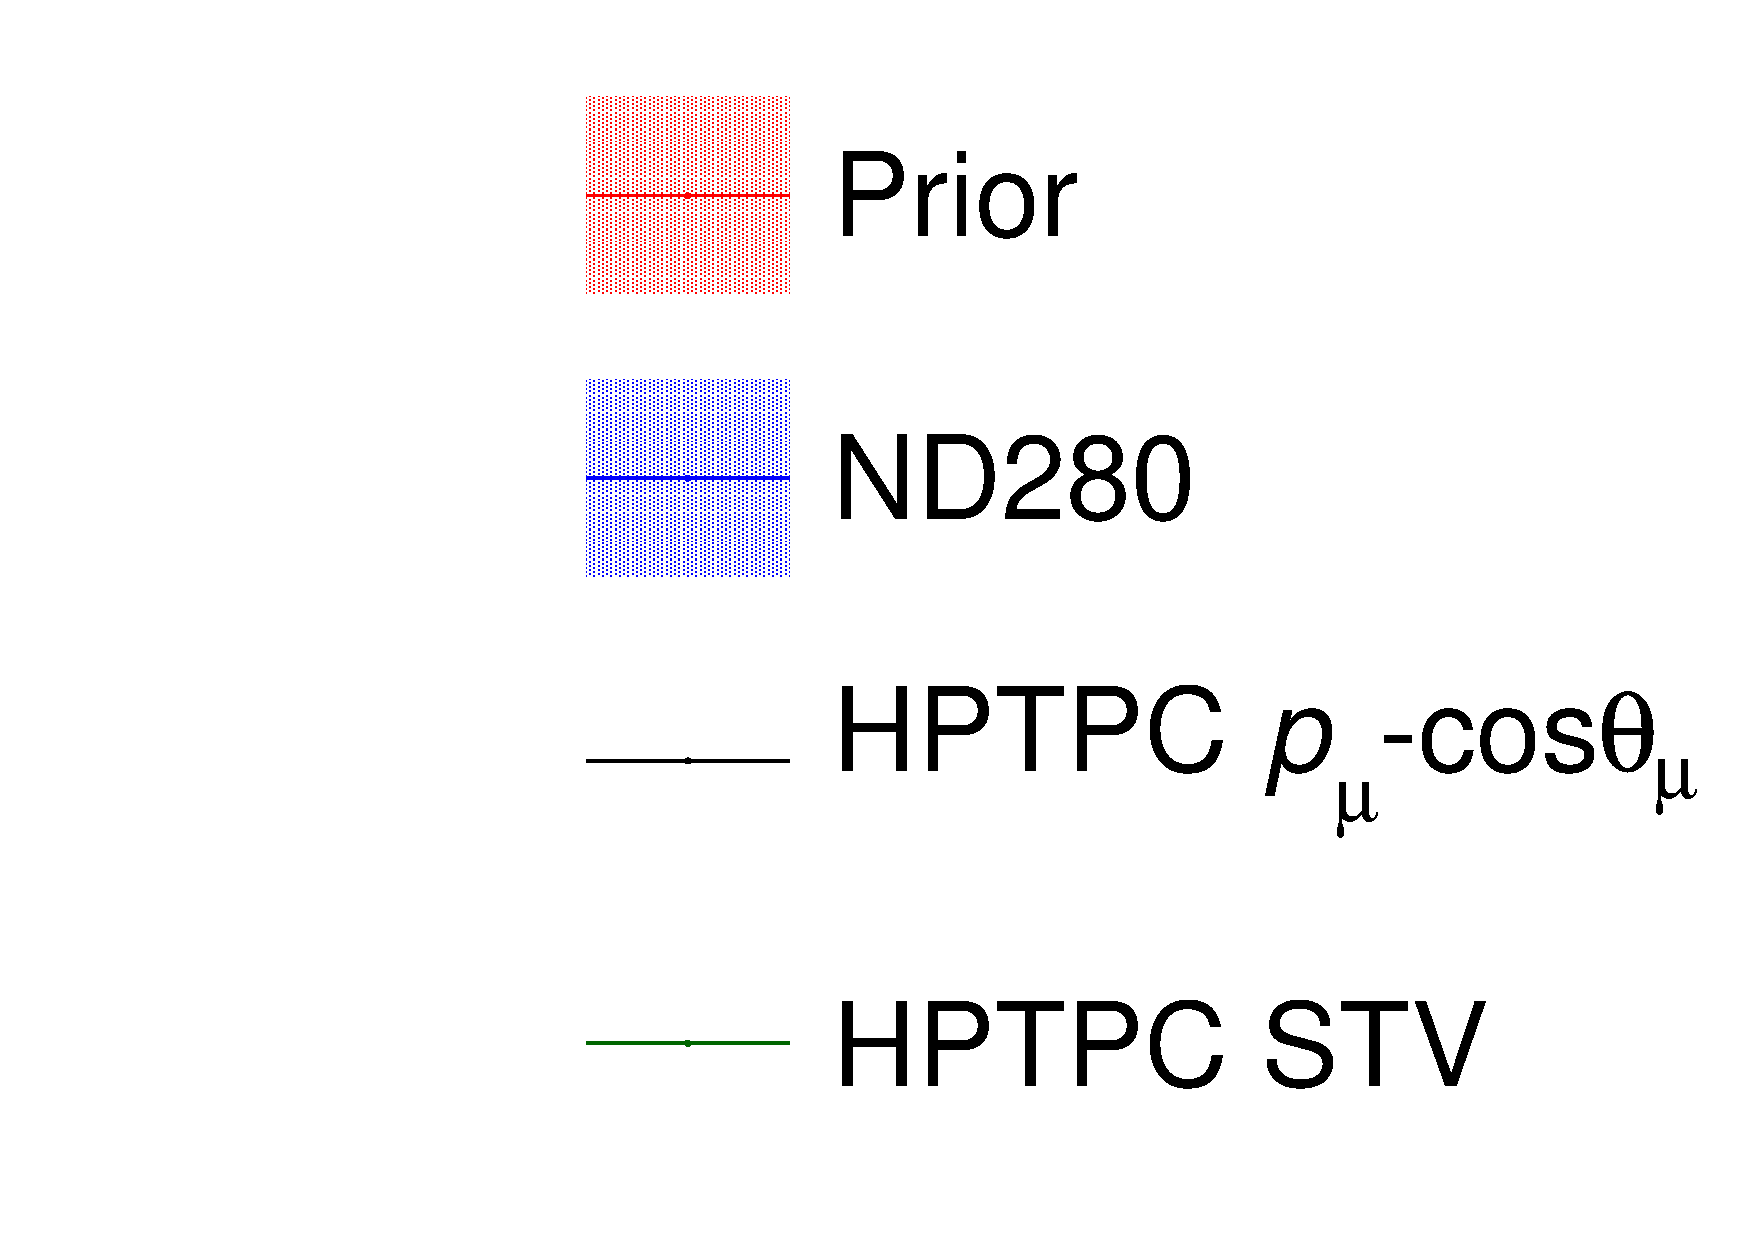
\includegraphics[width=1.0\linewidth, trim={5mm  90mm 0mm 0mm}, clip]{figs/hptpcfits_leg}	
\end{subfigure}
\begin{subfigure}{0.3\textwidth}
  \centering
  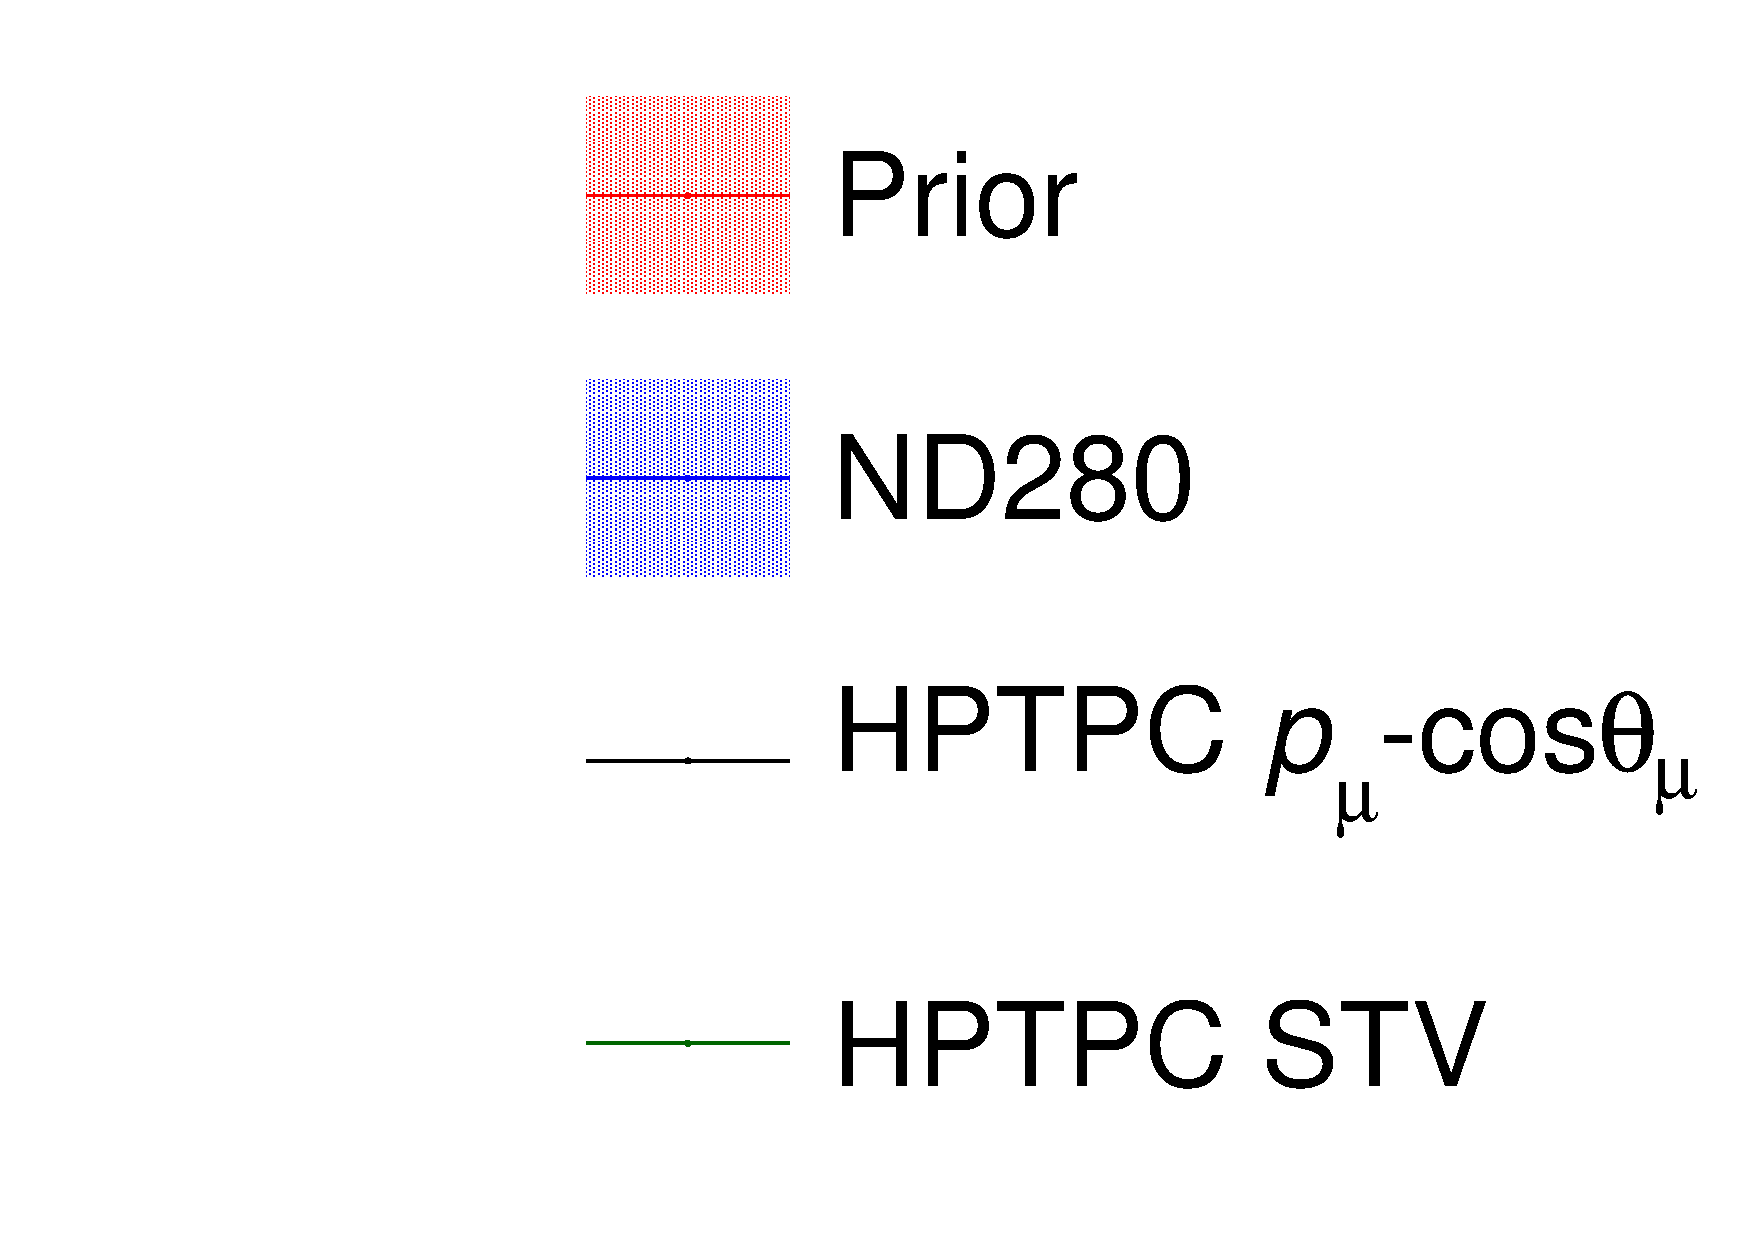
\includegraphics[width=1.0\linewidth, trim={5mm  0mm 0mm 95mm}, clip]{figs/hptpcfits_leg}	
\end{subfigure}
\begin{subfigure}{0.45\textwidth}
  \centering
  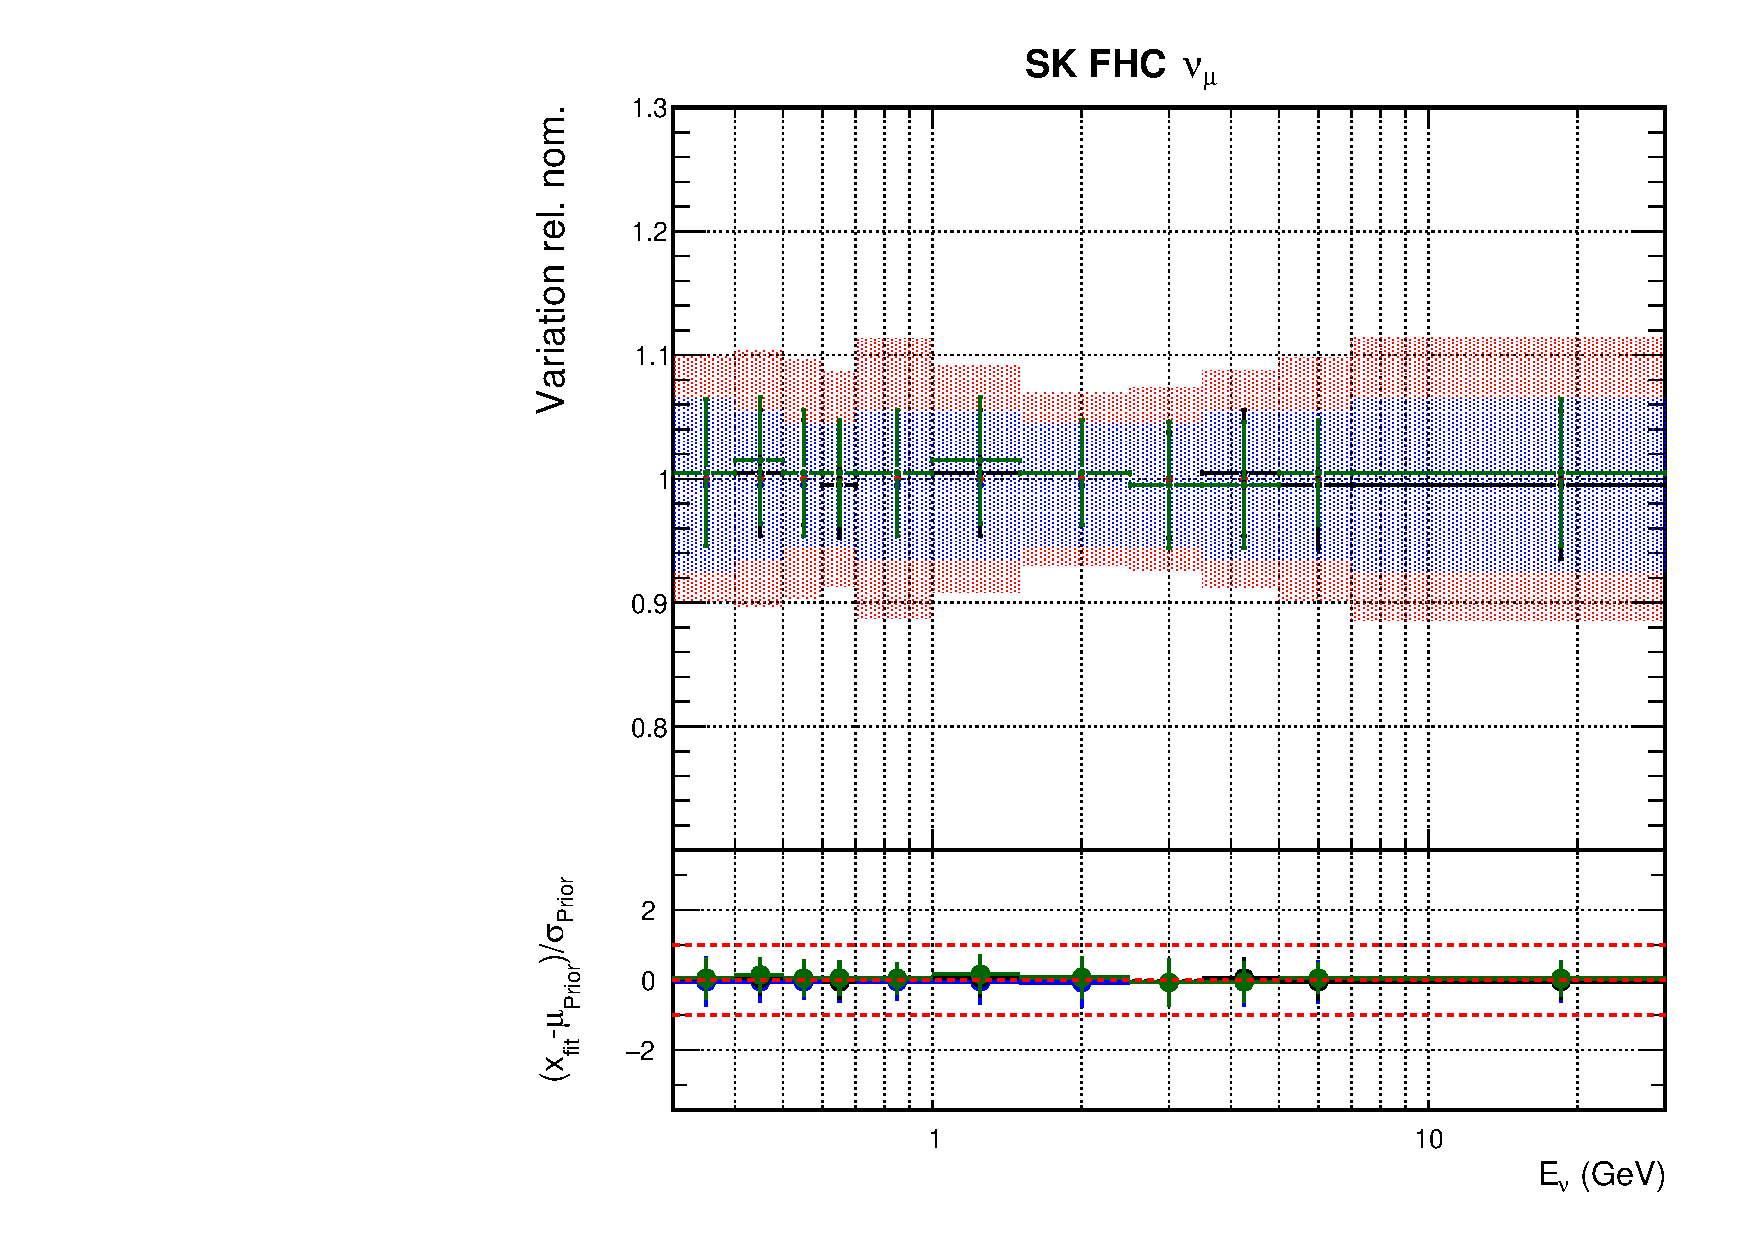
\includegraphics[width=0.75\linewidth]{figs/hptpcfitsflux_8}
  \caption{SK FHC $\nu_{\mu}$}
\end{subfigure}
\begin{subfigure}{0.45\textwidth}
  \centering
  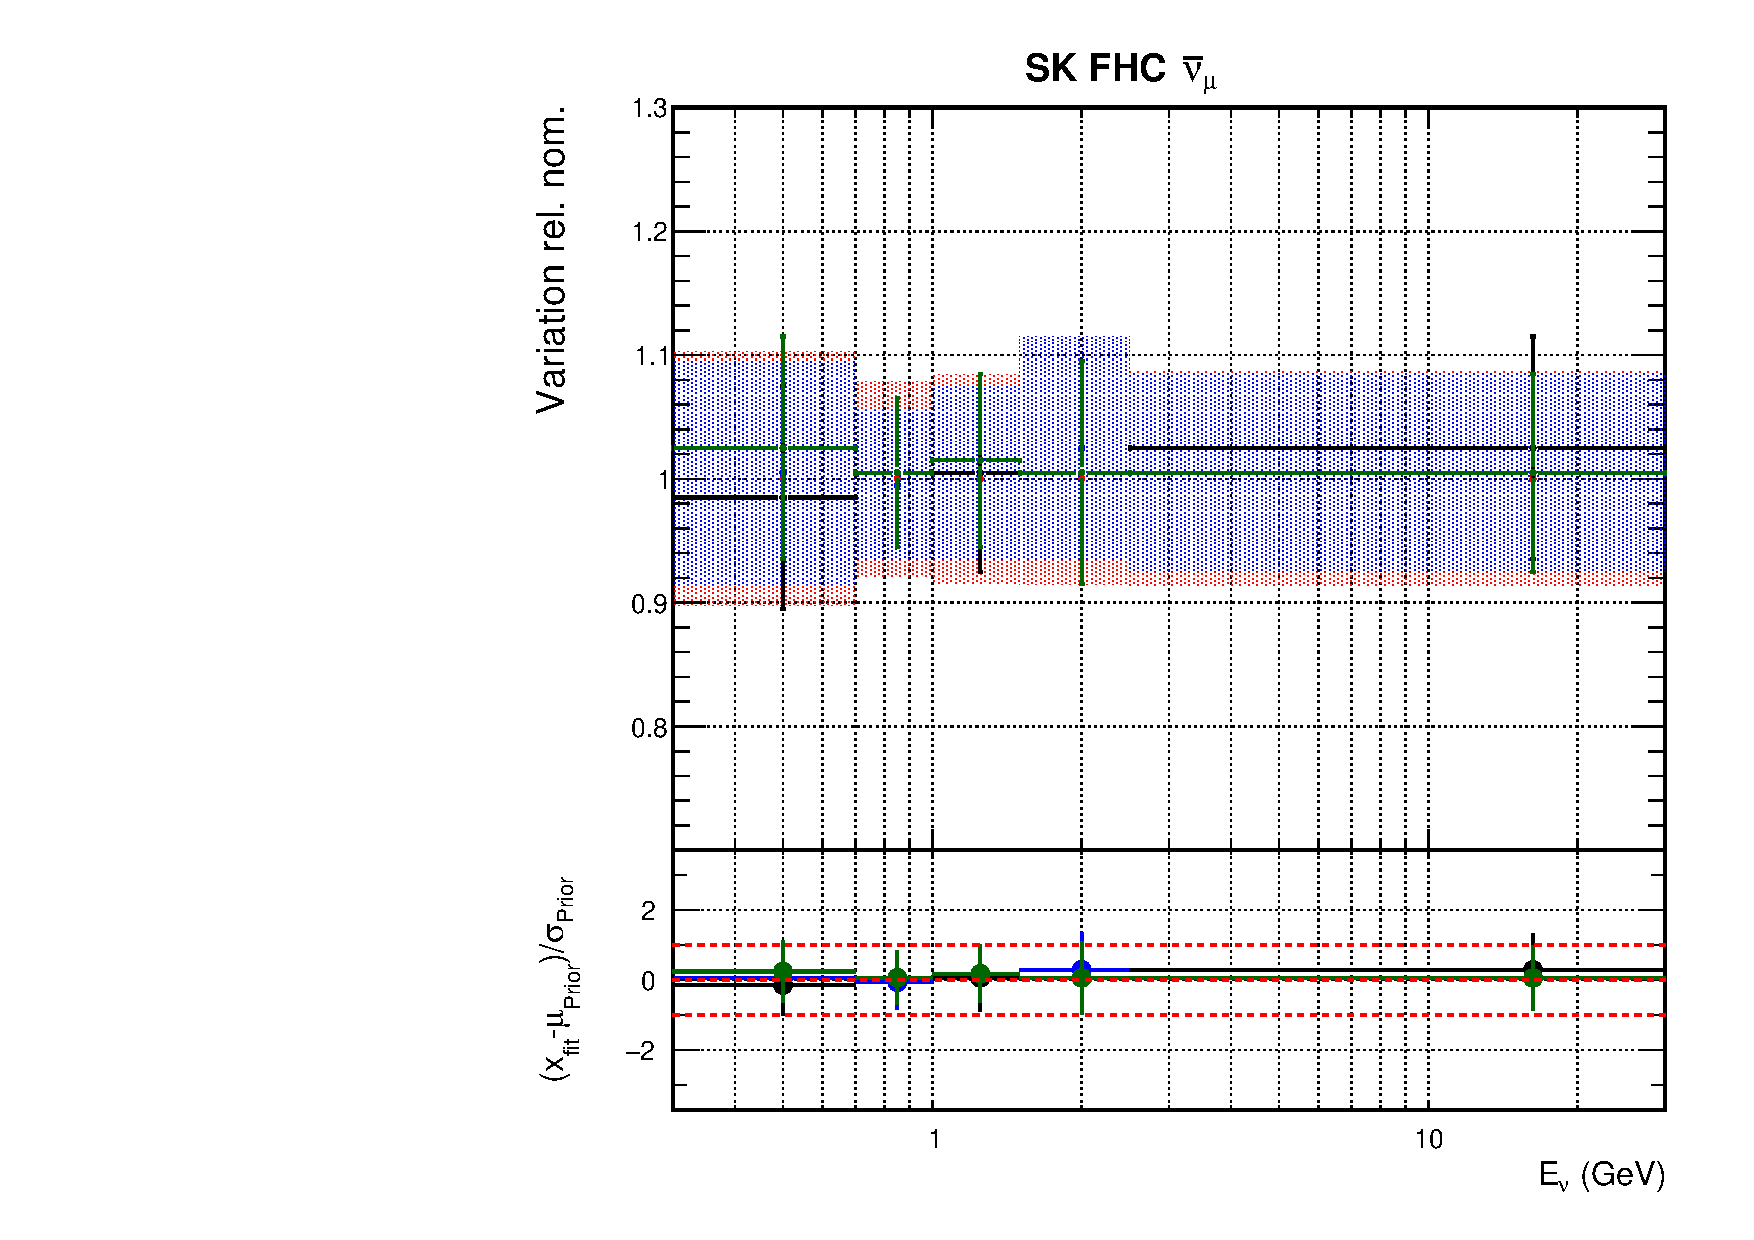
\includegraphics[width=0.75\linewidth]{figs/hptpcfitsflux_9}
  \caption{SK FHC $\bar{\nu_{\mu}}$}
\end{subfigure}
\begin{subfigure}{0.45\textwidth}
  \centering
  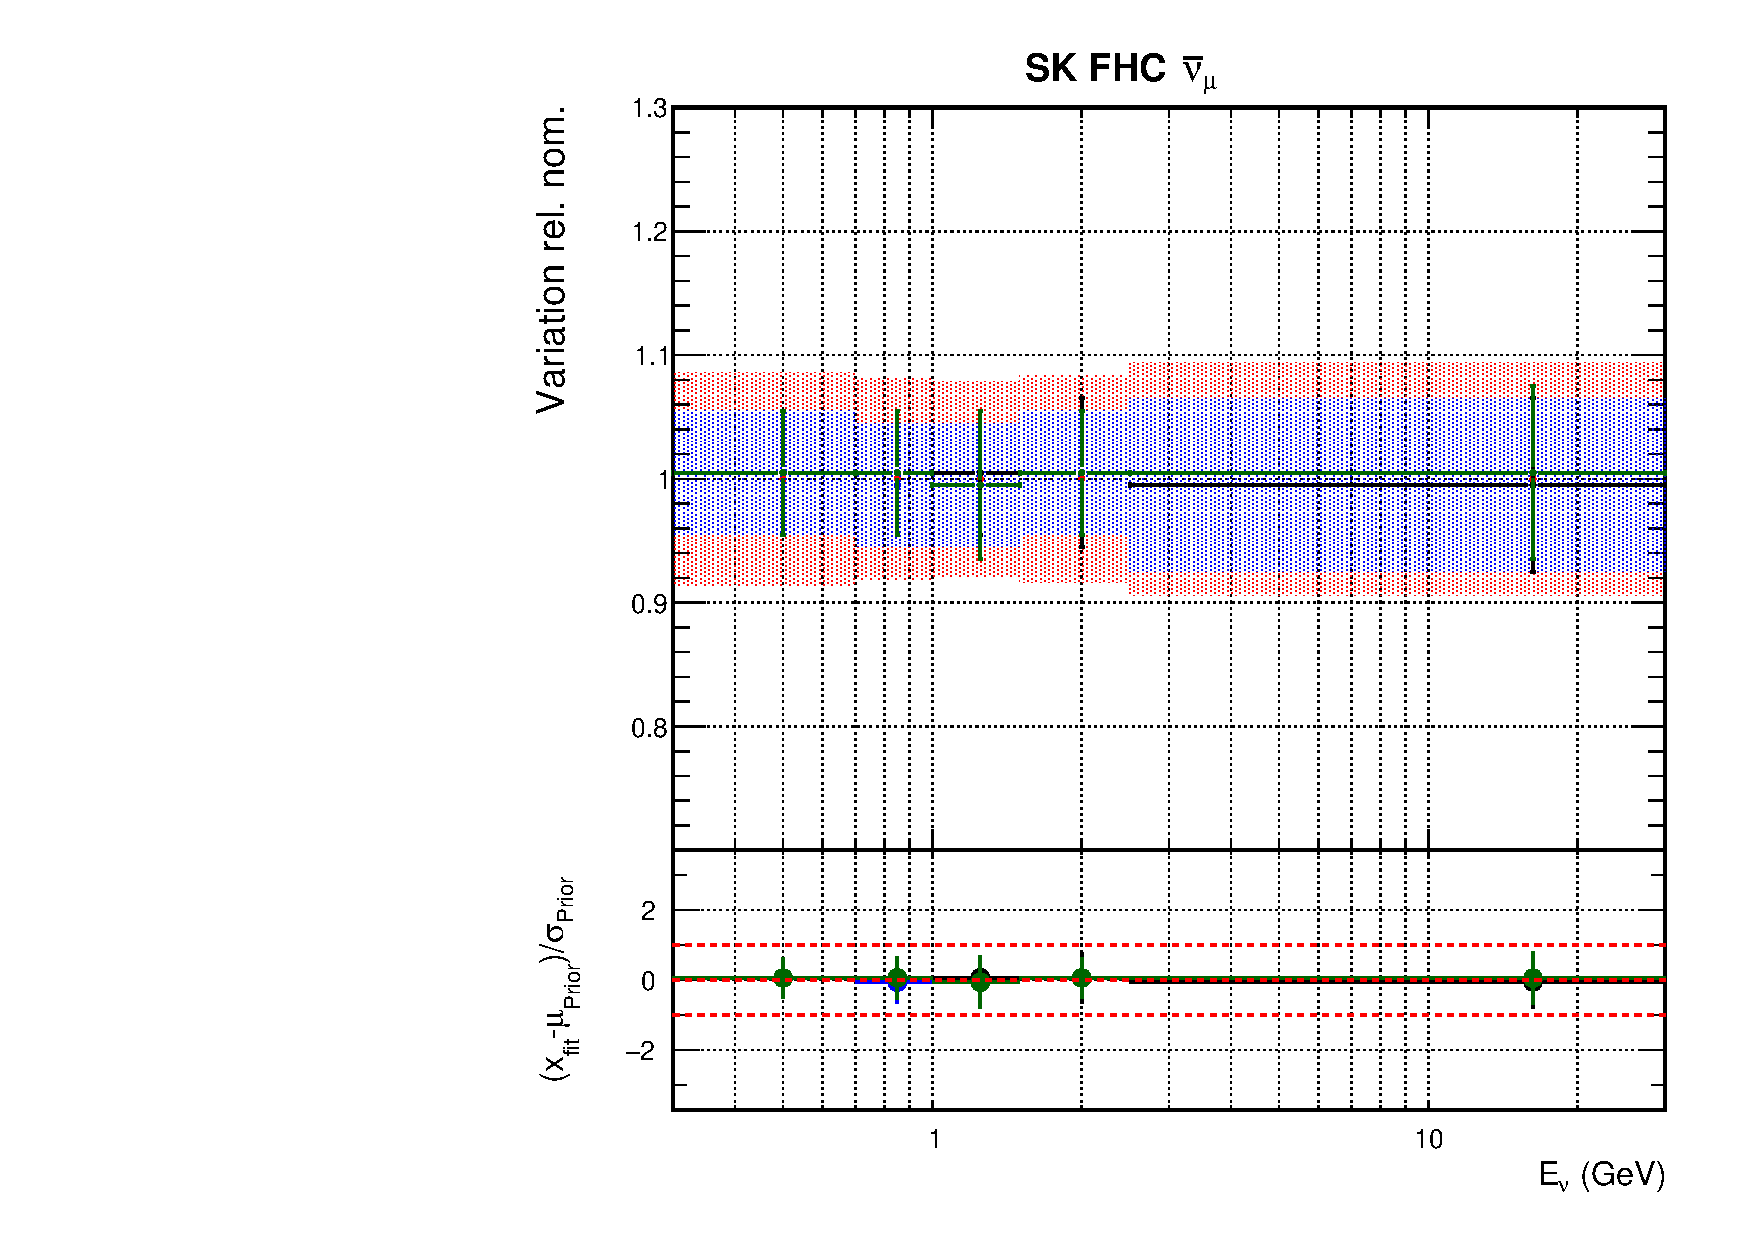
\includegraphics[width=0.75\linewidth]{figs/hptpcfitsflux_10}
  \caption{SK FHC $\nu_e$}
\end{subfigure}
\begin{subfigure}{0.45\textwidth}
  \centering
  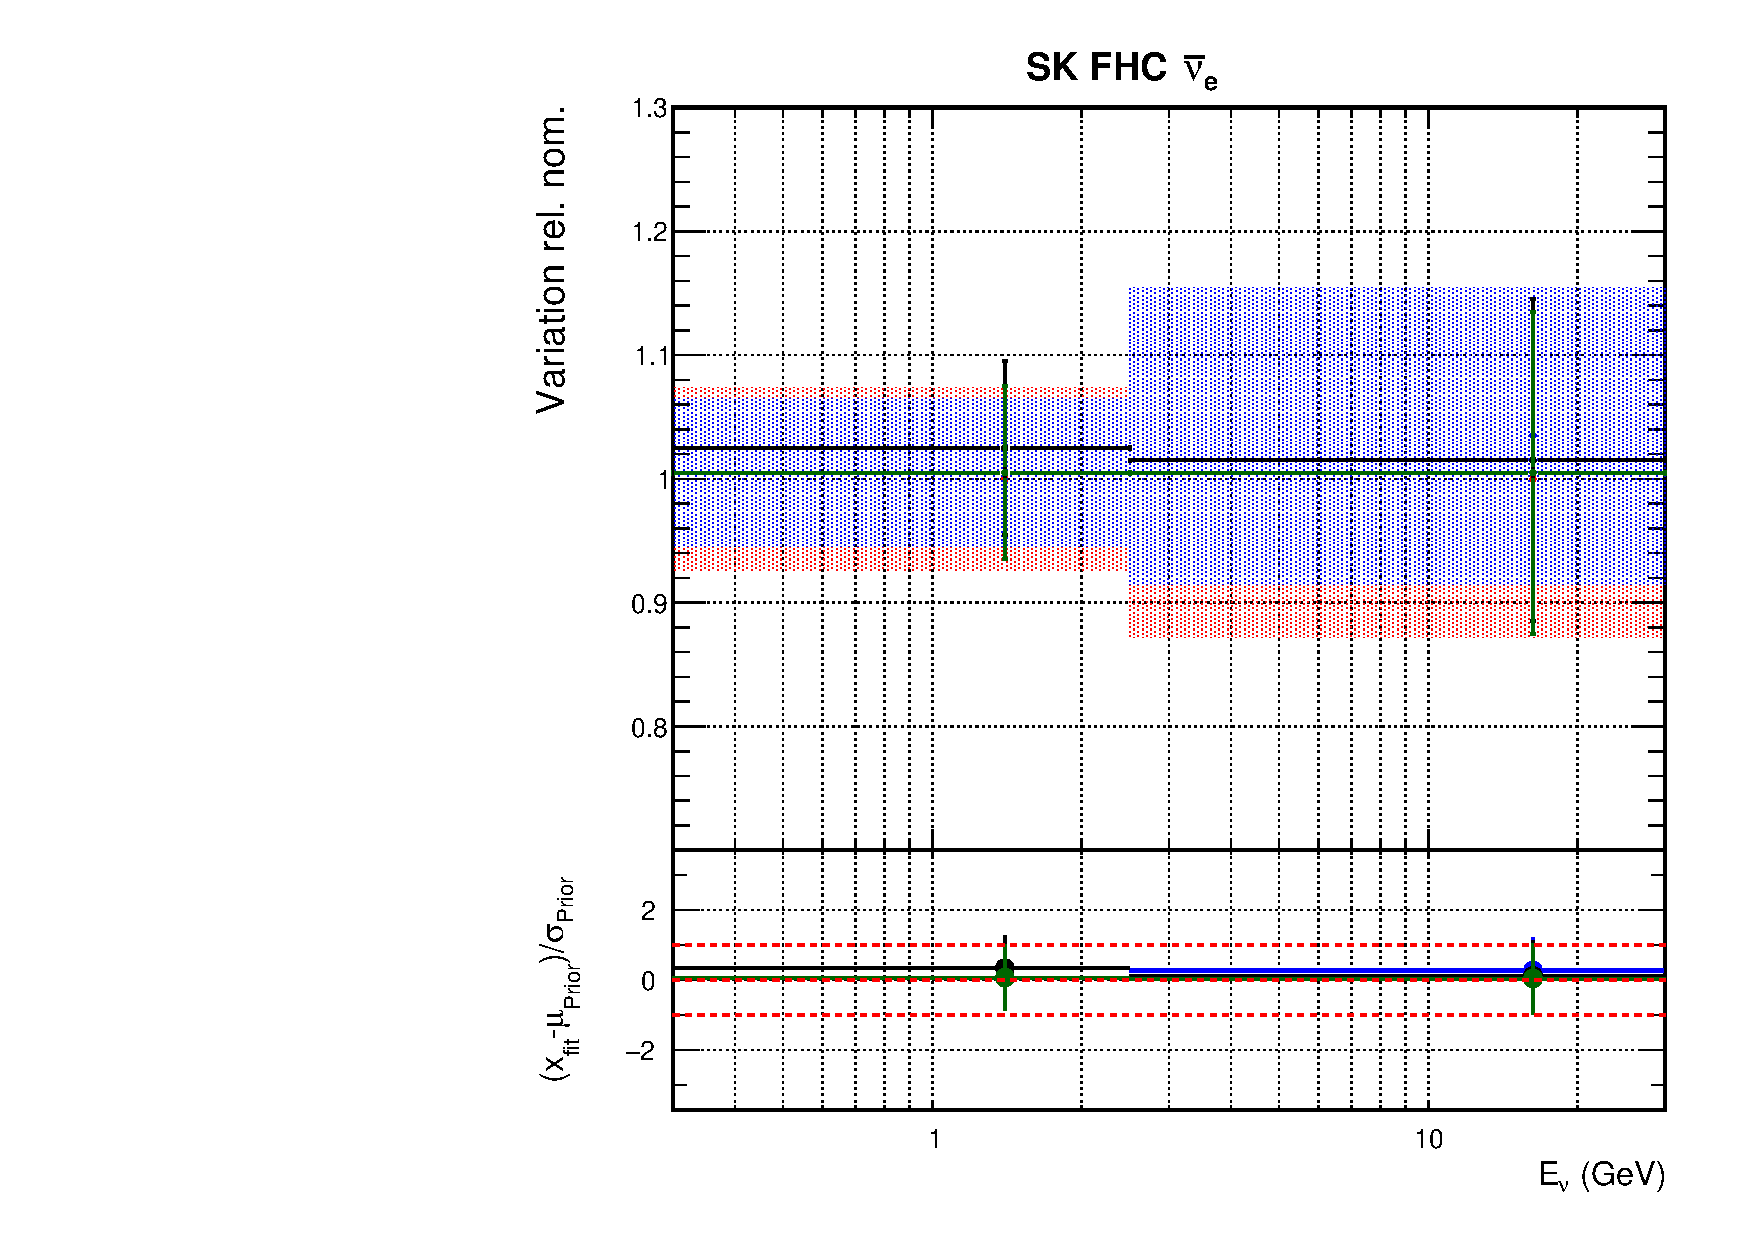
\includegraphics[width=0.75\linewidth]{figs/hptpcfitsflux_11}
  \caption{SK FHC $\bar{\nu_e}$}
\end{subfigure}
\begin{subfigure}{0.45\textwidth}
  \centering
  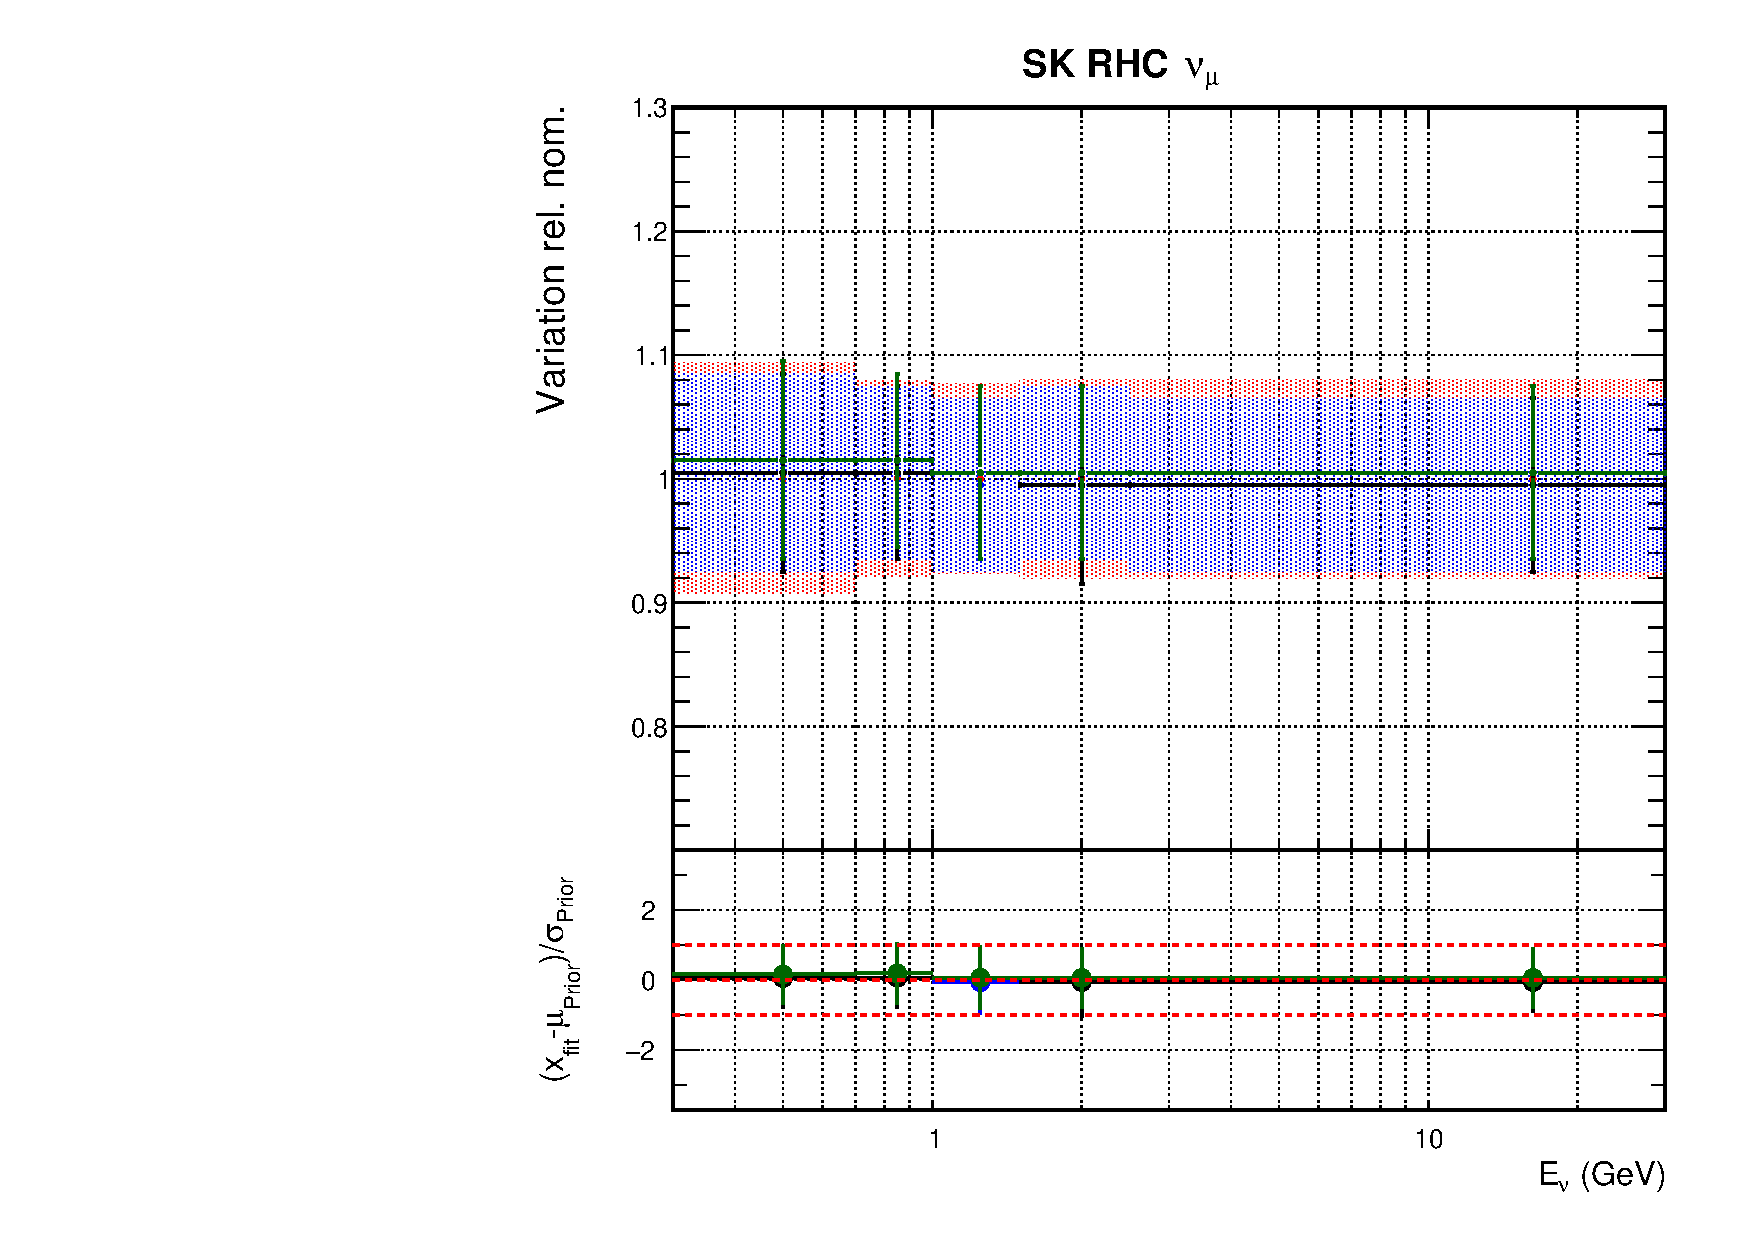
\includegraphics[width=0.75\linewidth]{figs/hptpcfitsflux_12}
  \caption{SK RHC $\nu_{\mu}$}
\end{subfigure}
\begin{subfigure}{0.45\textwidth}
  \centering
  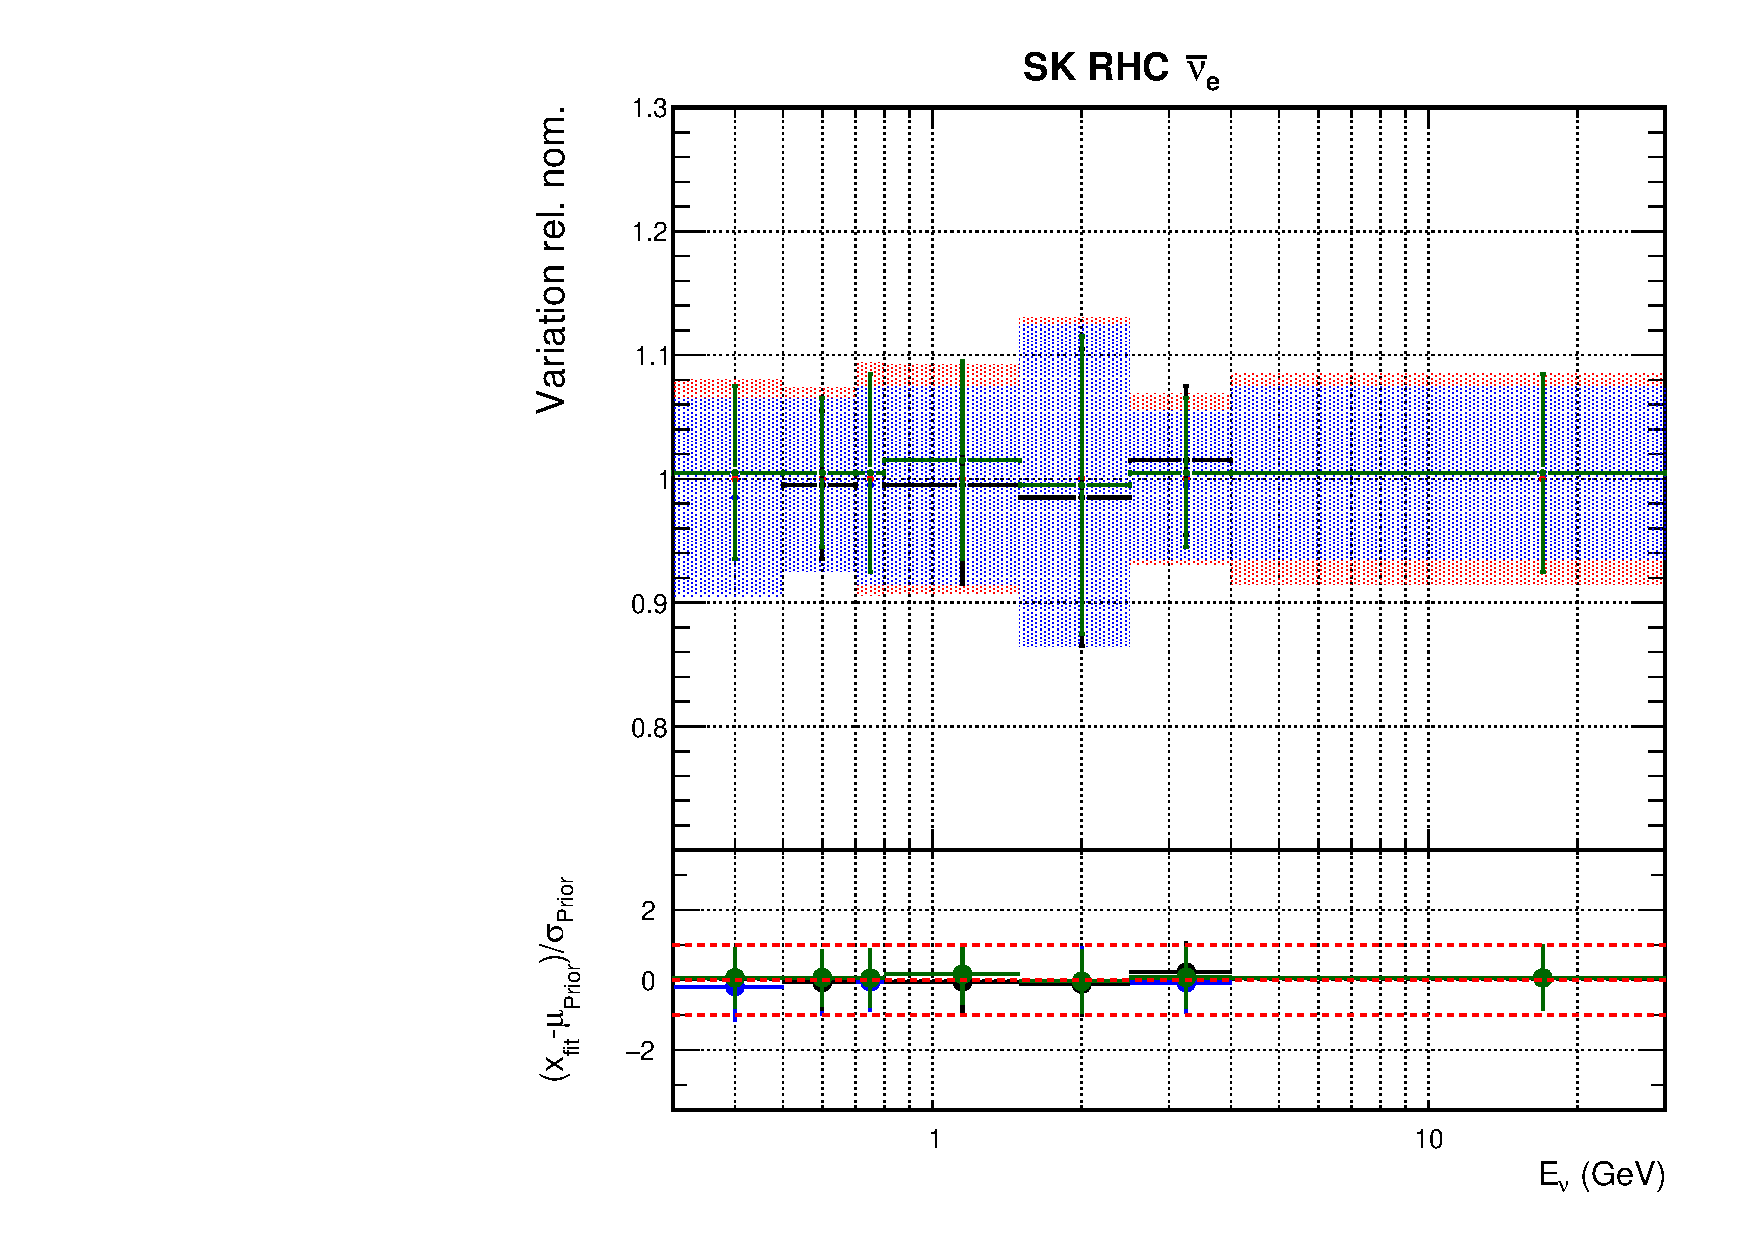
\includegraphics[width=0.75\linewidth]{figs/hptpcfitsflux_13}
  \caption{SK RHC $\bar{\nu_{\mu}}$}
\end{subfigure}
\begin{subfigure}{0.45\textwidth}
  \centering
  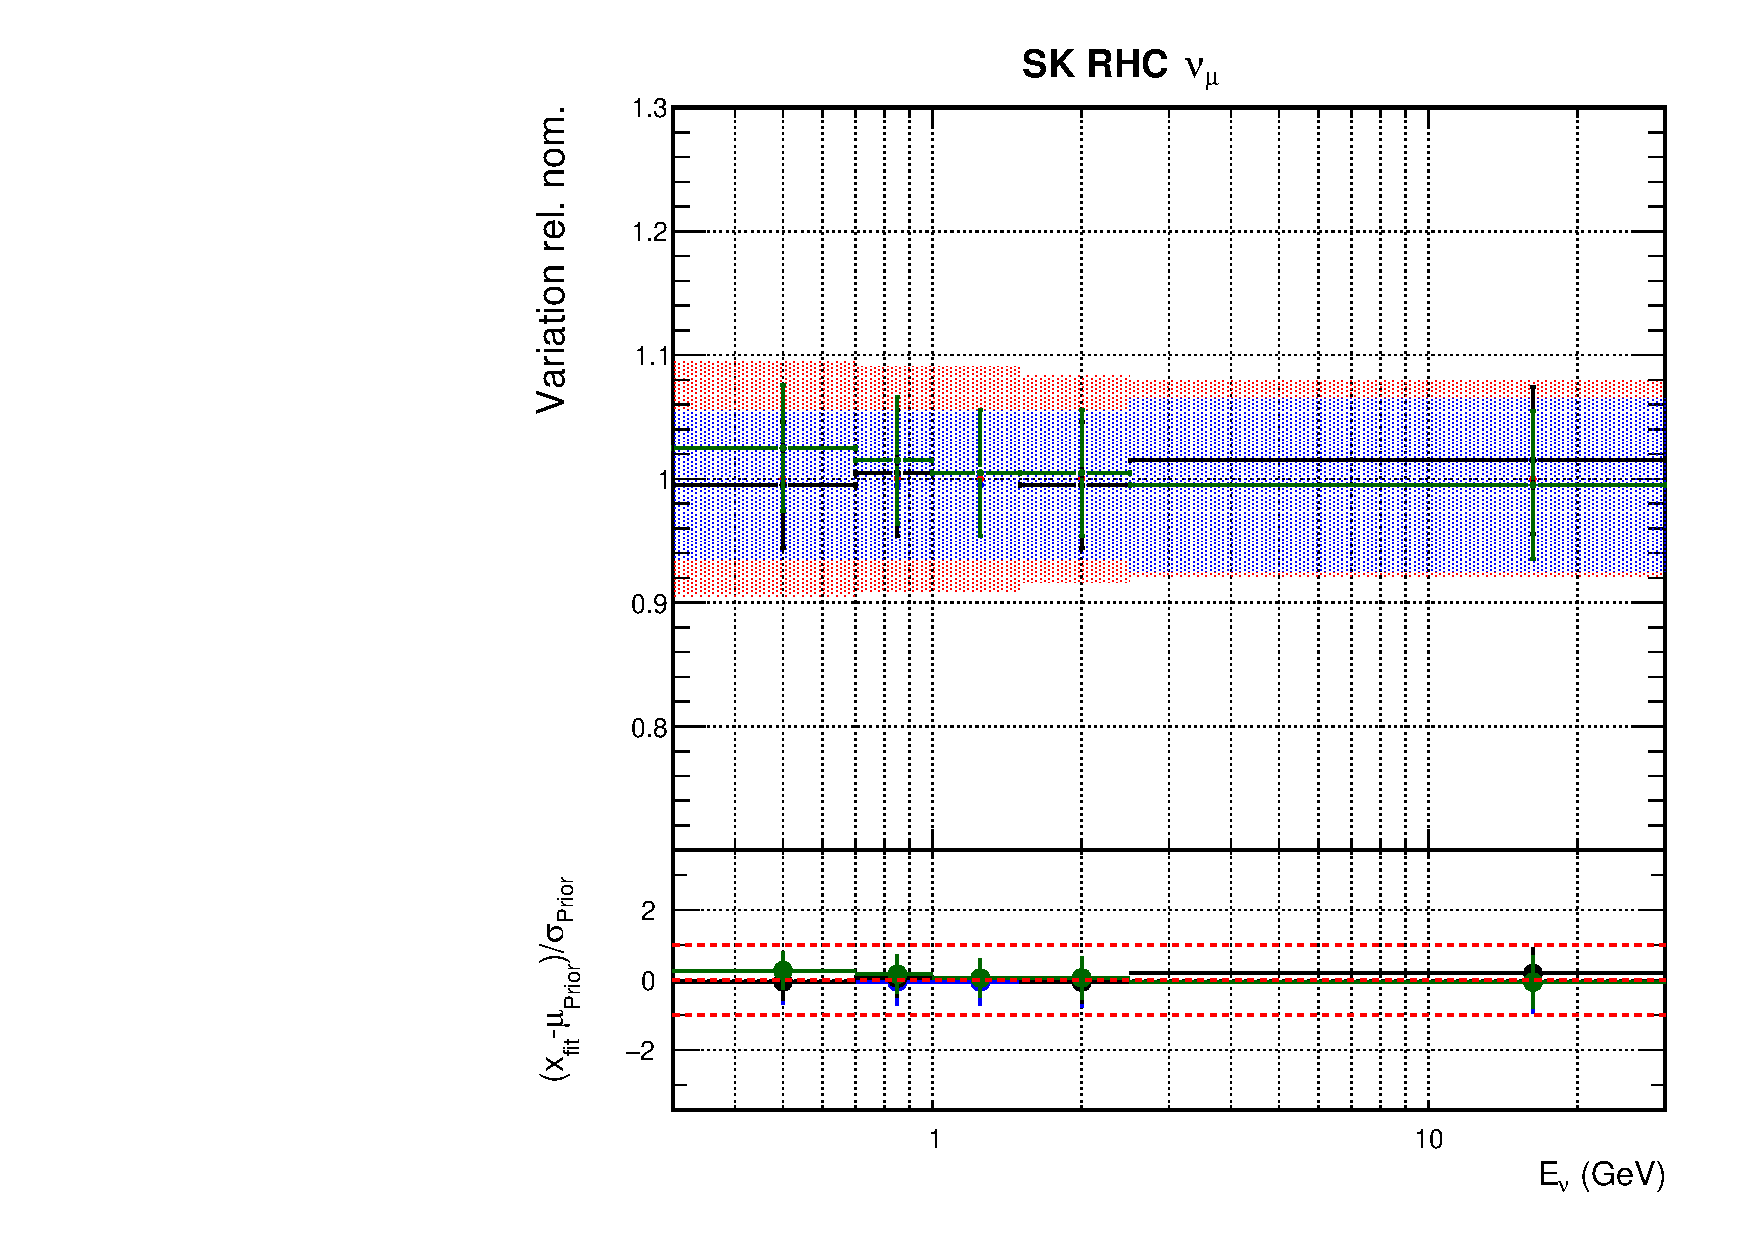
\includegraphics[width=0.75\linewidth]{figs/hptpcfitsflux_14}
  \caption{SK RHC $\nu_{e}$}
\end{subfigure}
\begin{subfigure}{0.45\textwidth}
  \centering
  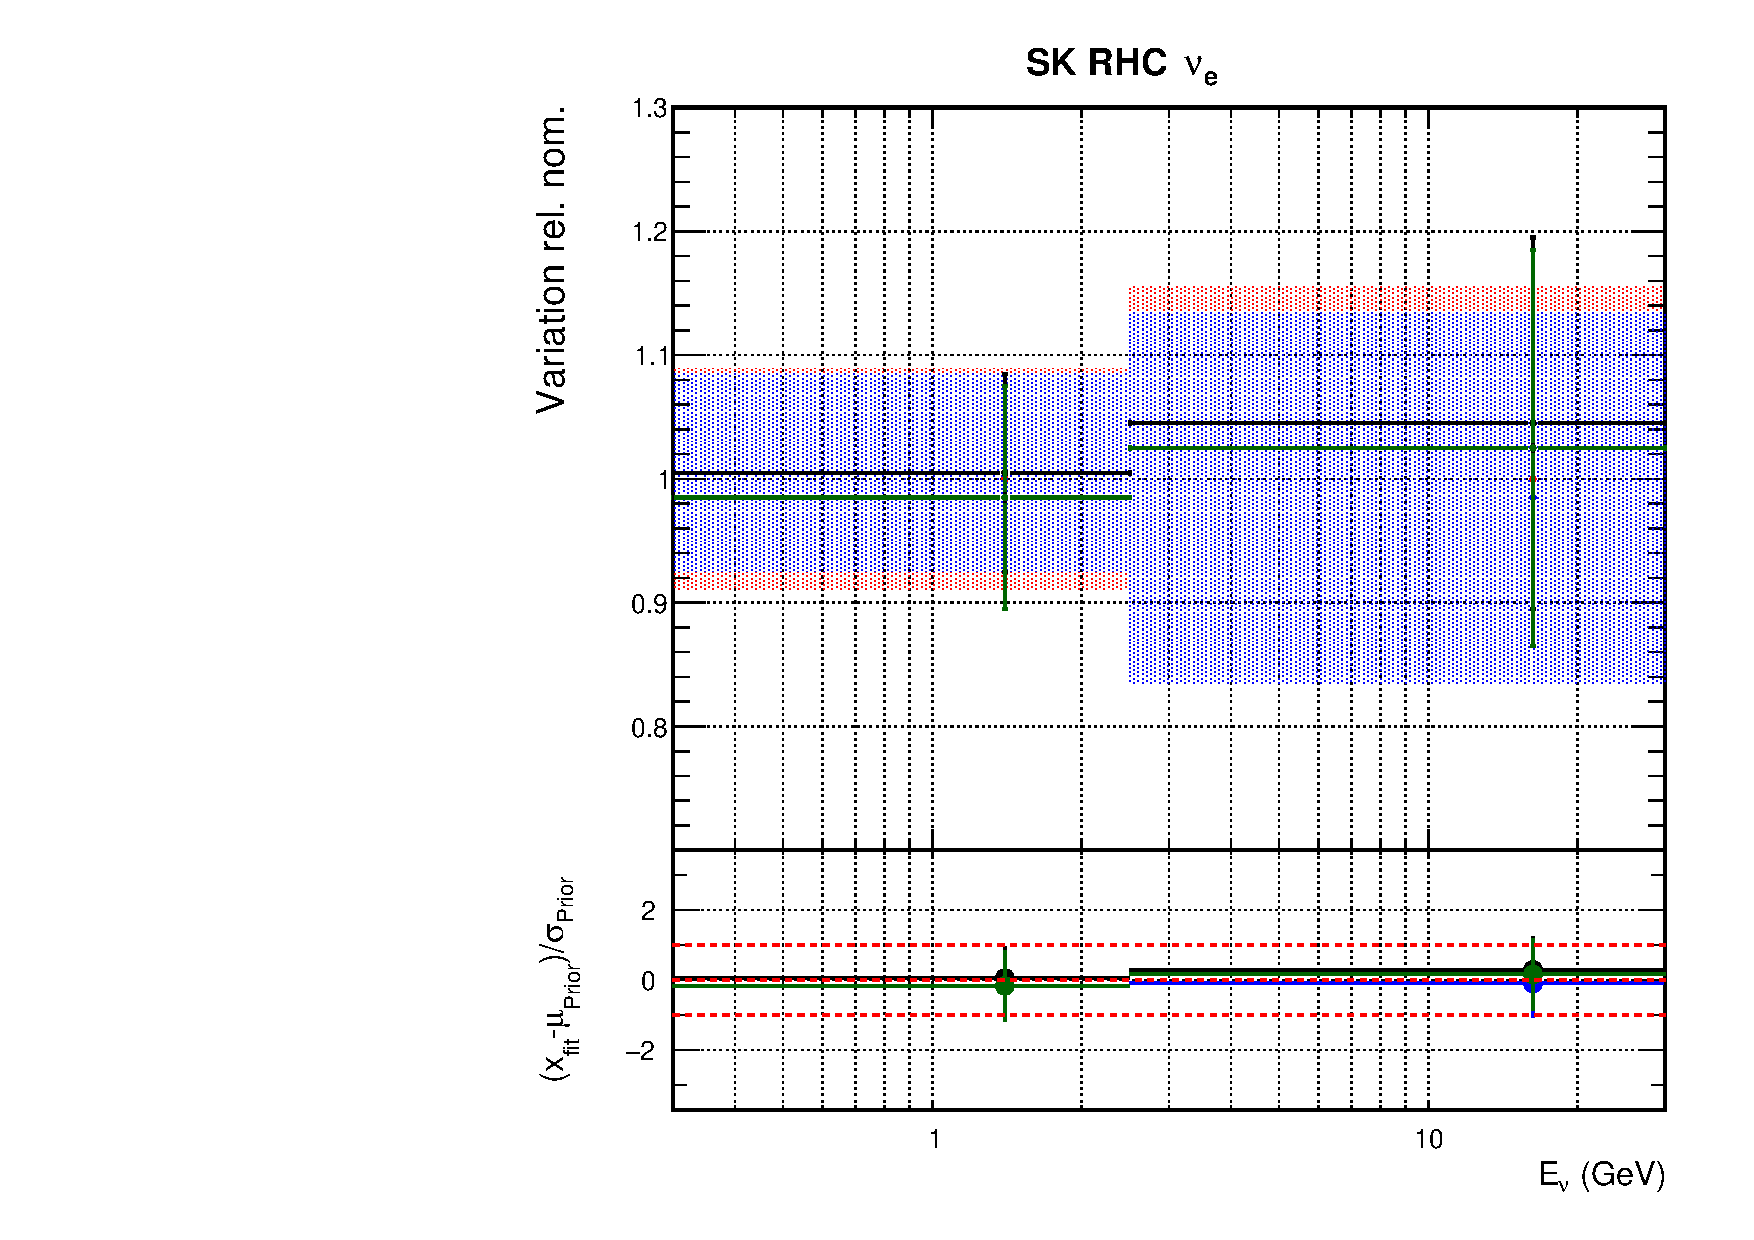
\includegraphics[width=0.75\linewidth]{figs/hptpcfitsflux_15}
  \caption{SK RHC $\bar{\nu_e}$}
\end{subfigure}
\caption{SK flux parameters for ND280 $p_{\mu}$-cos$\theta_{\mu}$, HPTPC $p_{\mu}$-cos$\theta_{\mu}$, and HPTPC mixed STV fits.}
\label{fig:hptpcfluxSK}
\end{figure}

\begin{figure}
\centering
\begin{subfigure}{0.3\textwidth}
  \centering
  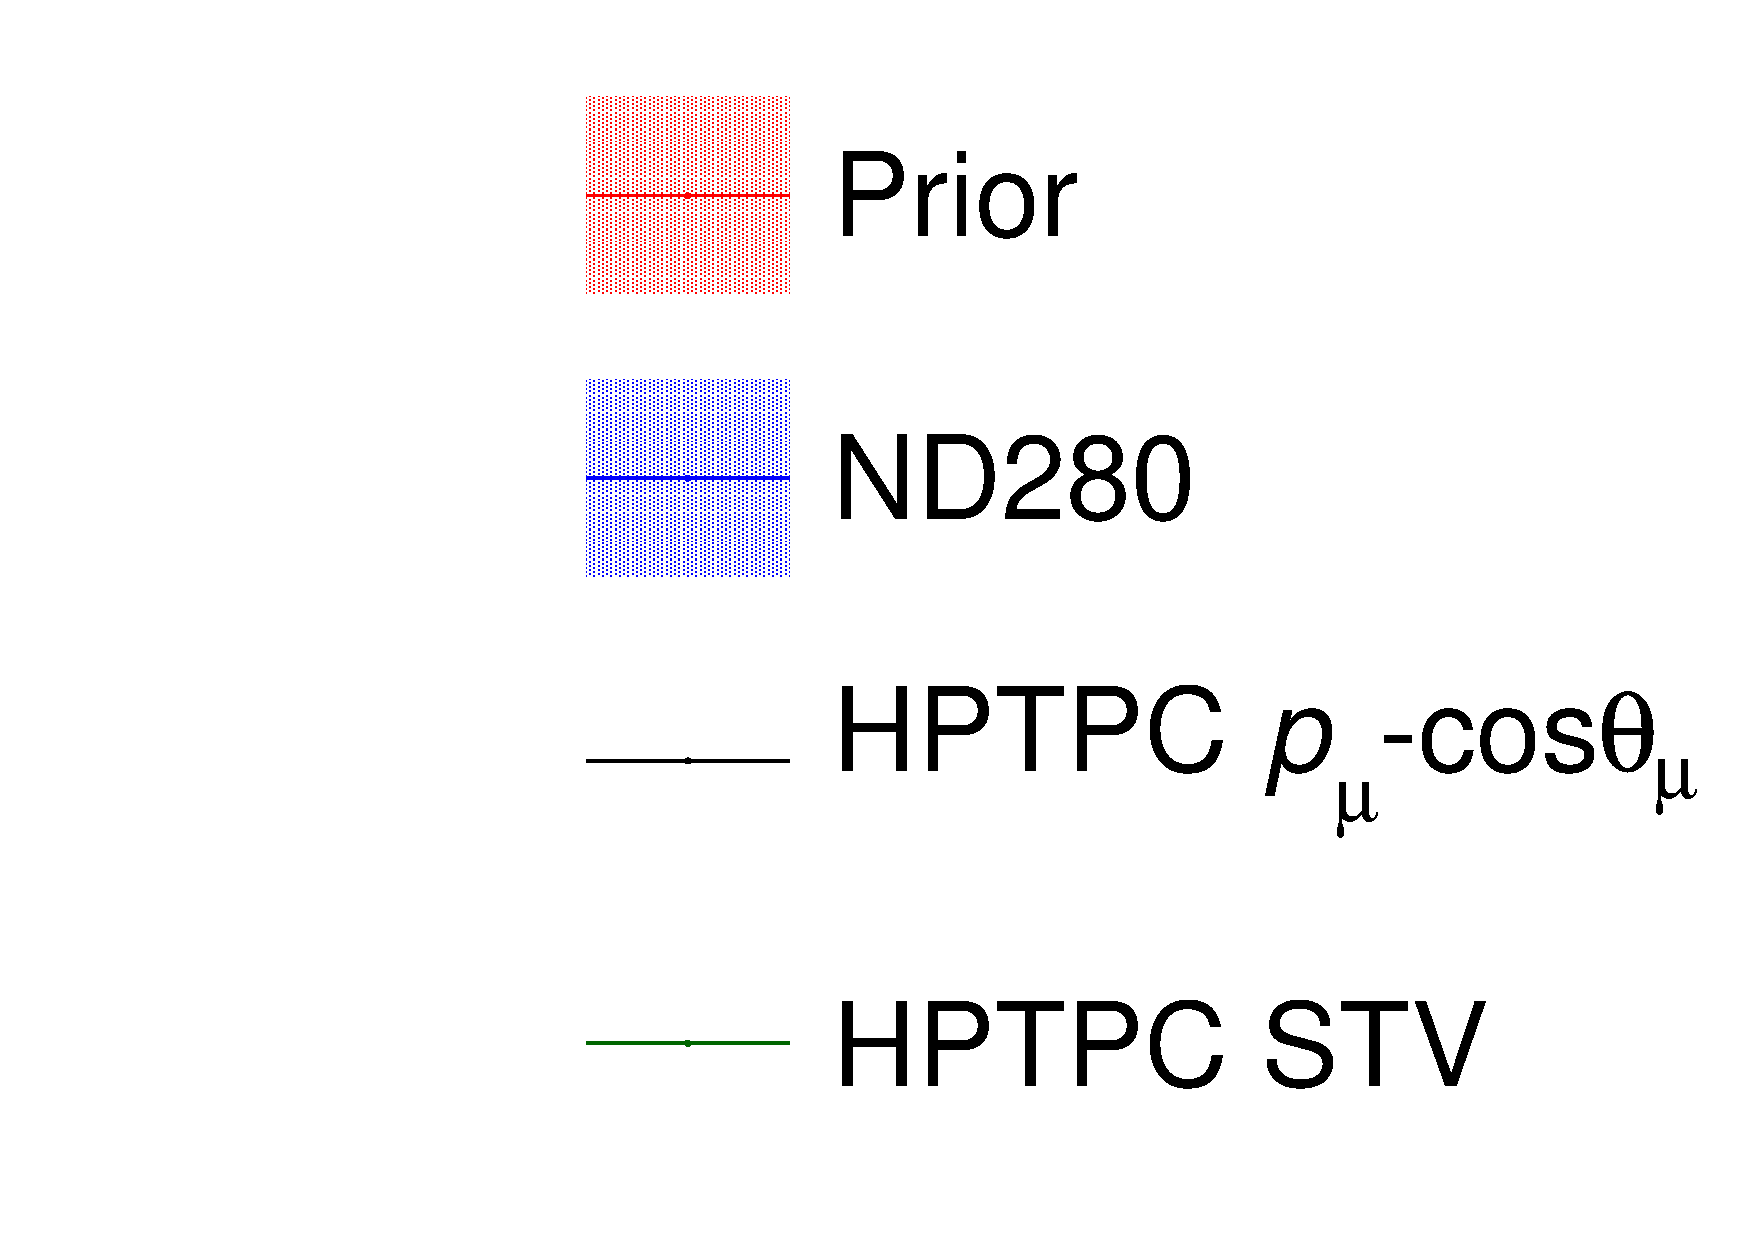
\includegraphics[width=1.0\linewidth, trim={5mm  90mm 0mm 0mm}, clip]{figs/hptpcfits_leg}	
\end{subfigure}
\begin{subfigure}{0.3\textwidth}
  \centering
  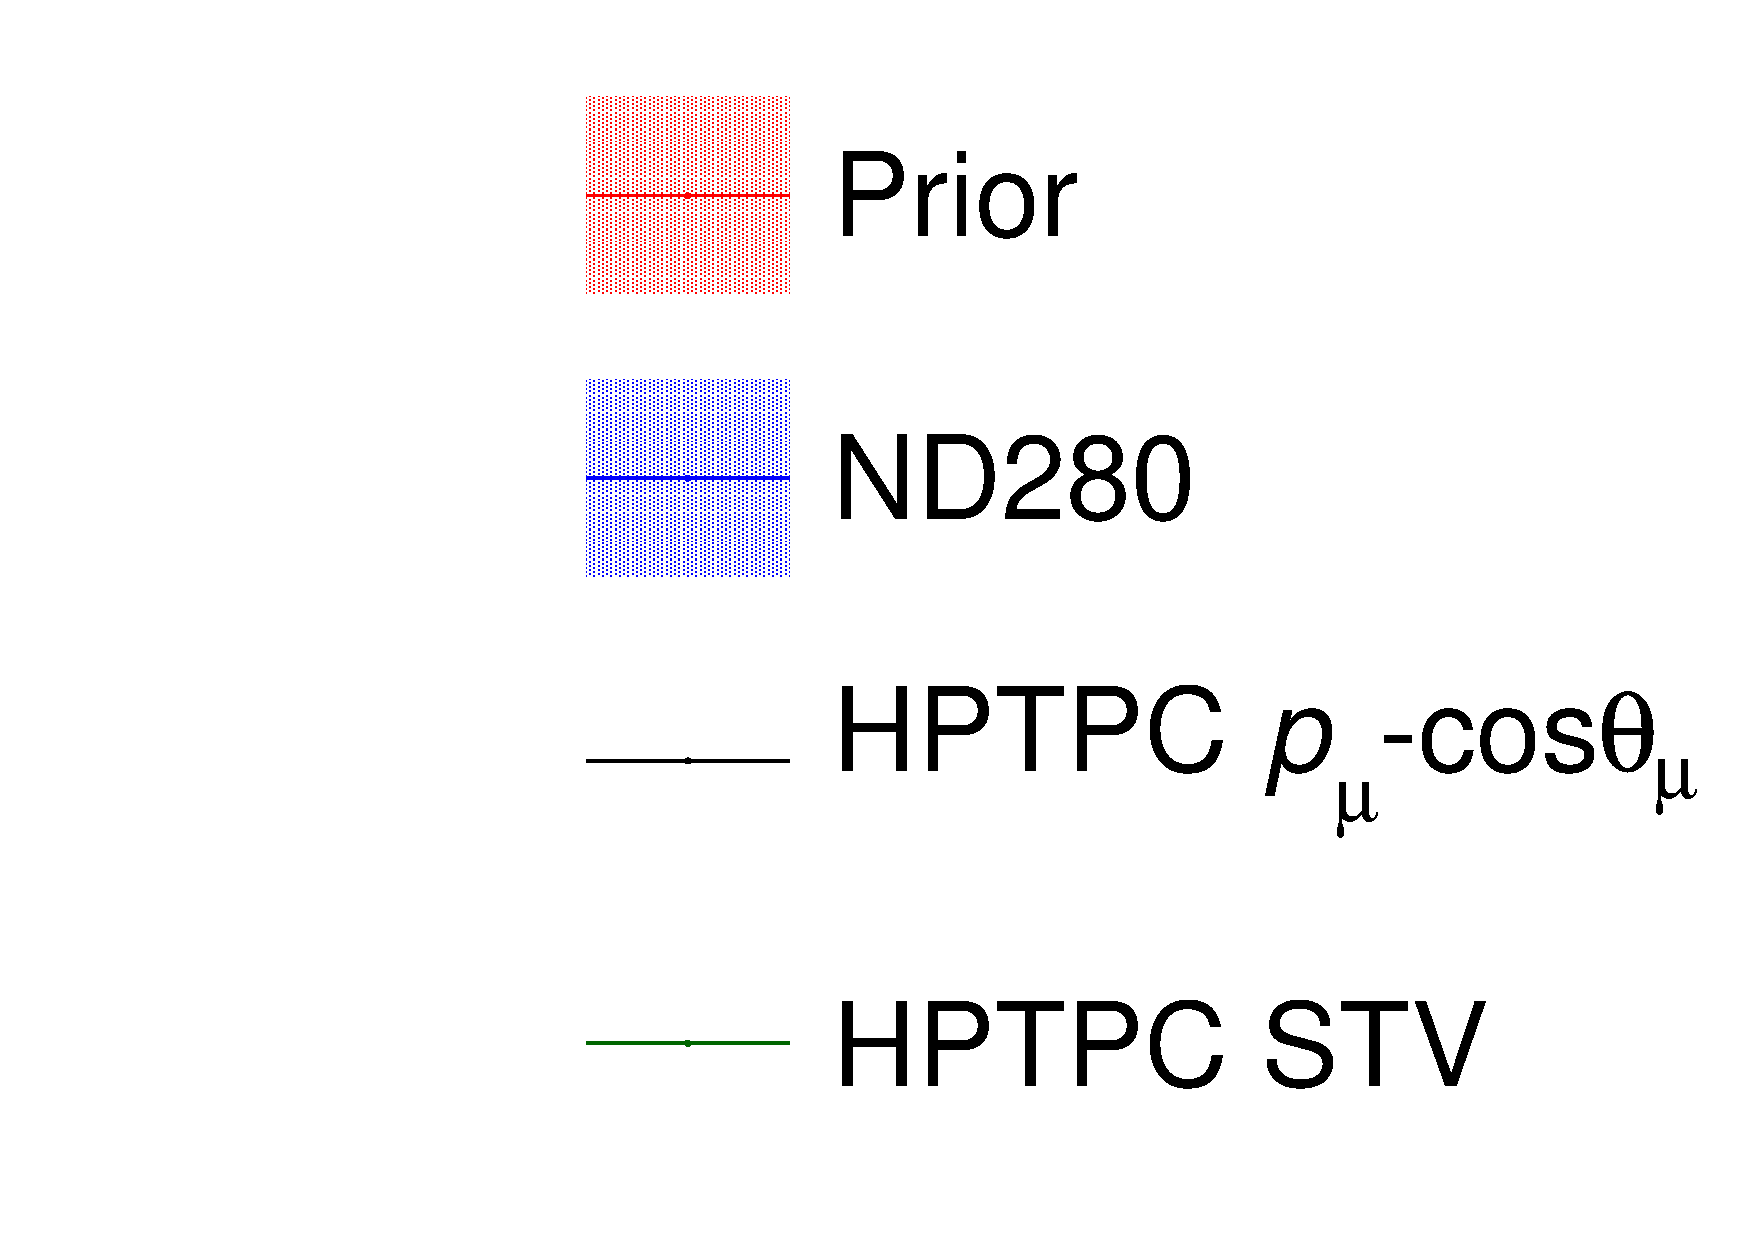
\includegraphics[width=1.0\linewidth, trim={5mm  0mm 0mm 95mm}, clip]{figs/hptpcfits_leg}	
\end{subfigure}
\begin{subfigure}{0.49\textwidth}
  \centering
  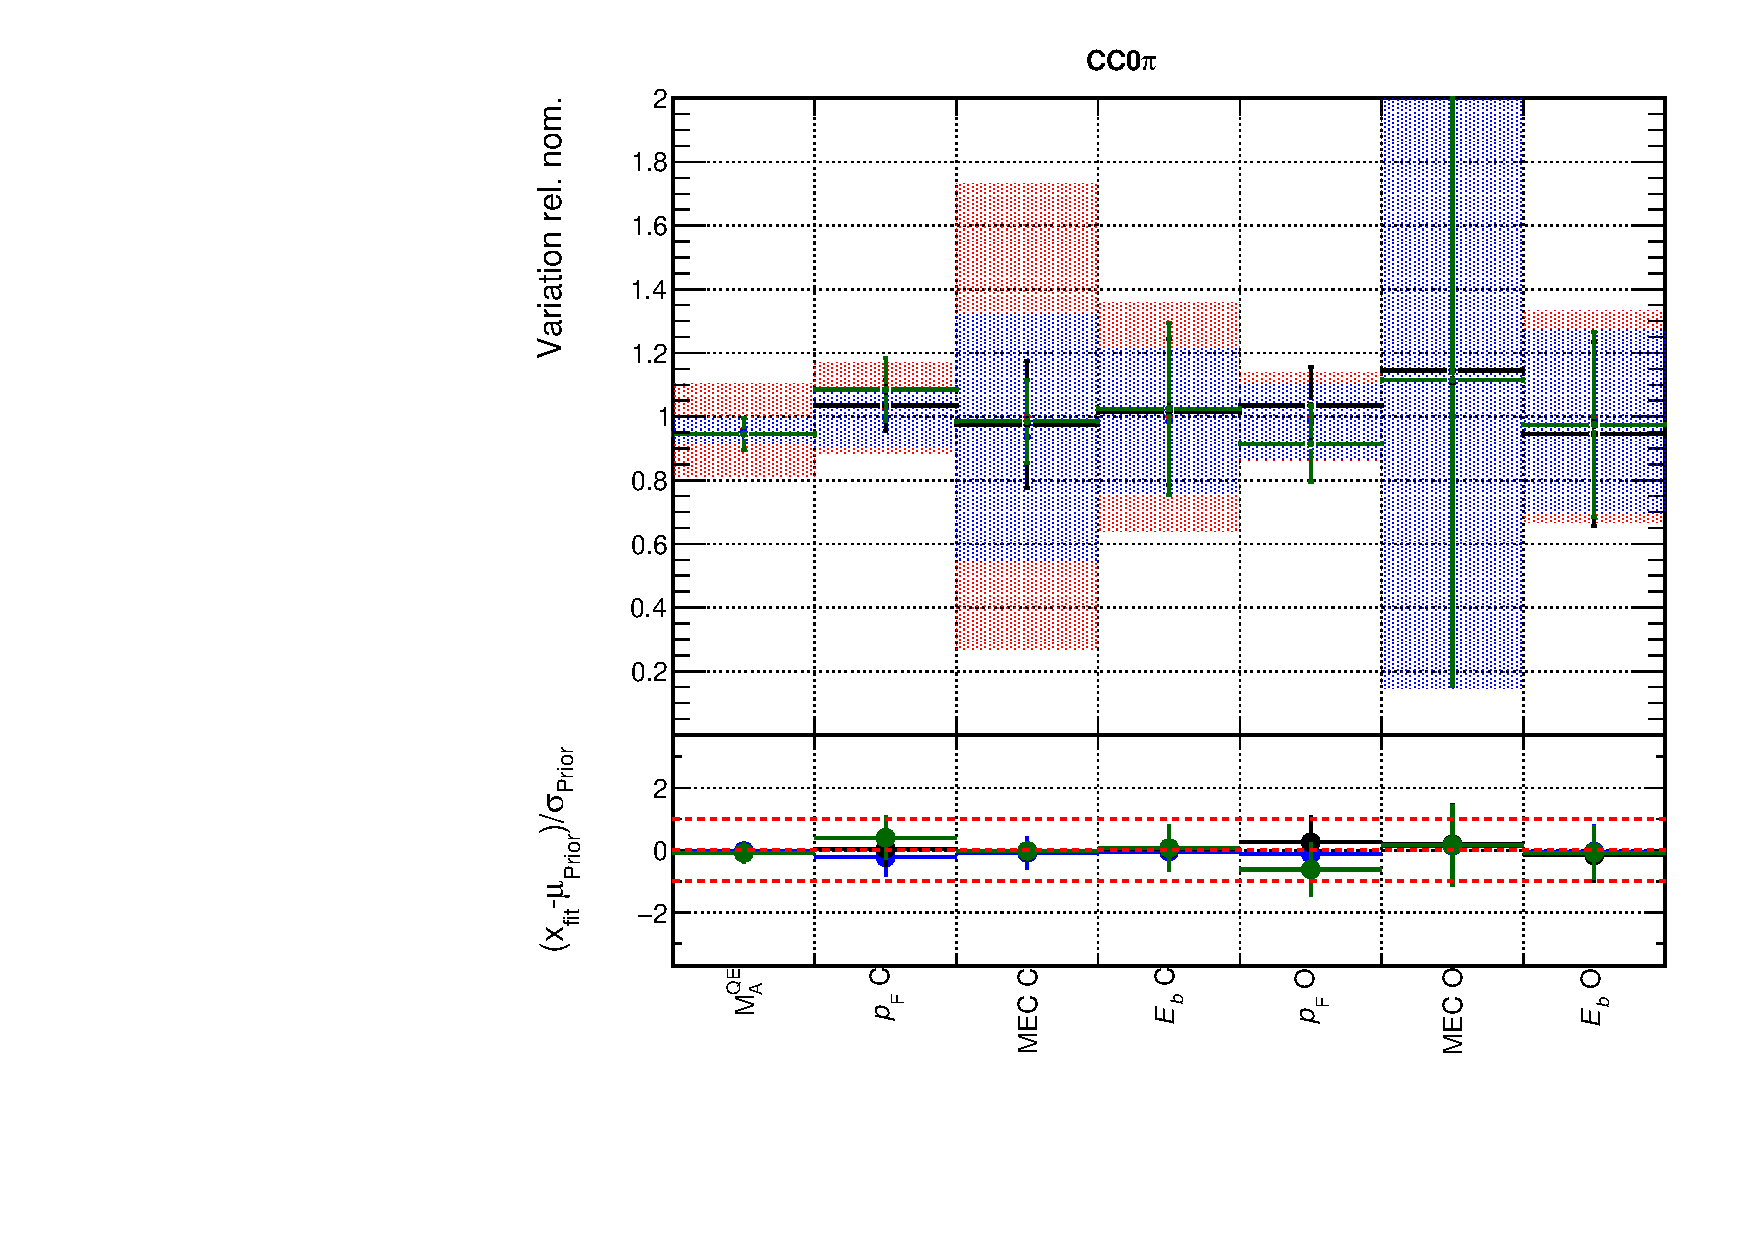
\includegraphics[width=0.95\linewidth]{figs/hptpcfitsxsec_1}
  \caption{CC0$\pi$}
\end{subfigure}
\begin{subfigure}{0.49\textwidth}
  \centering
  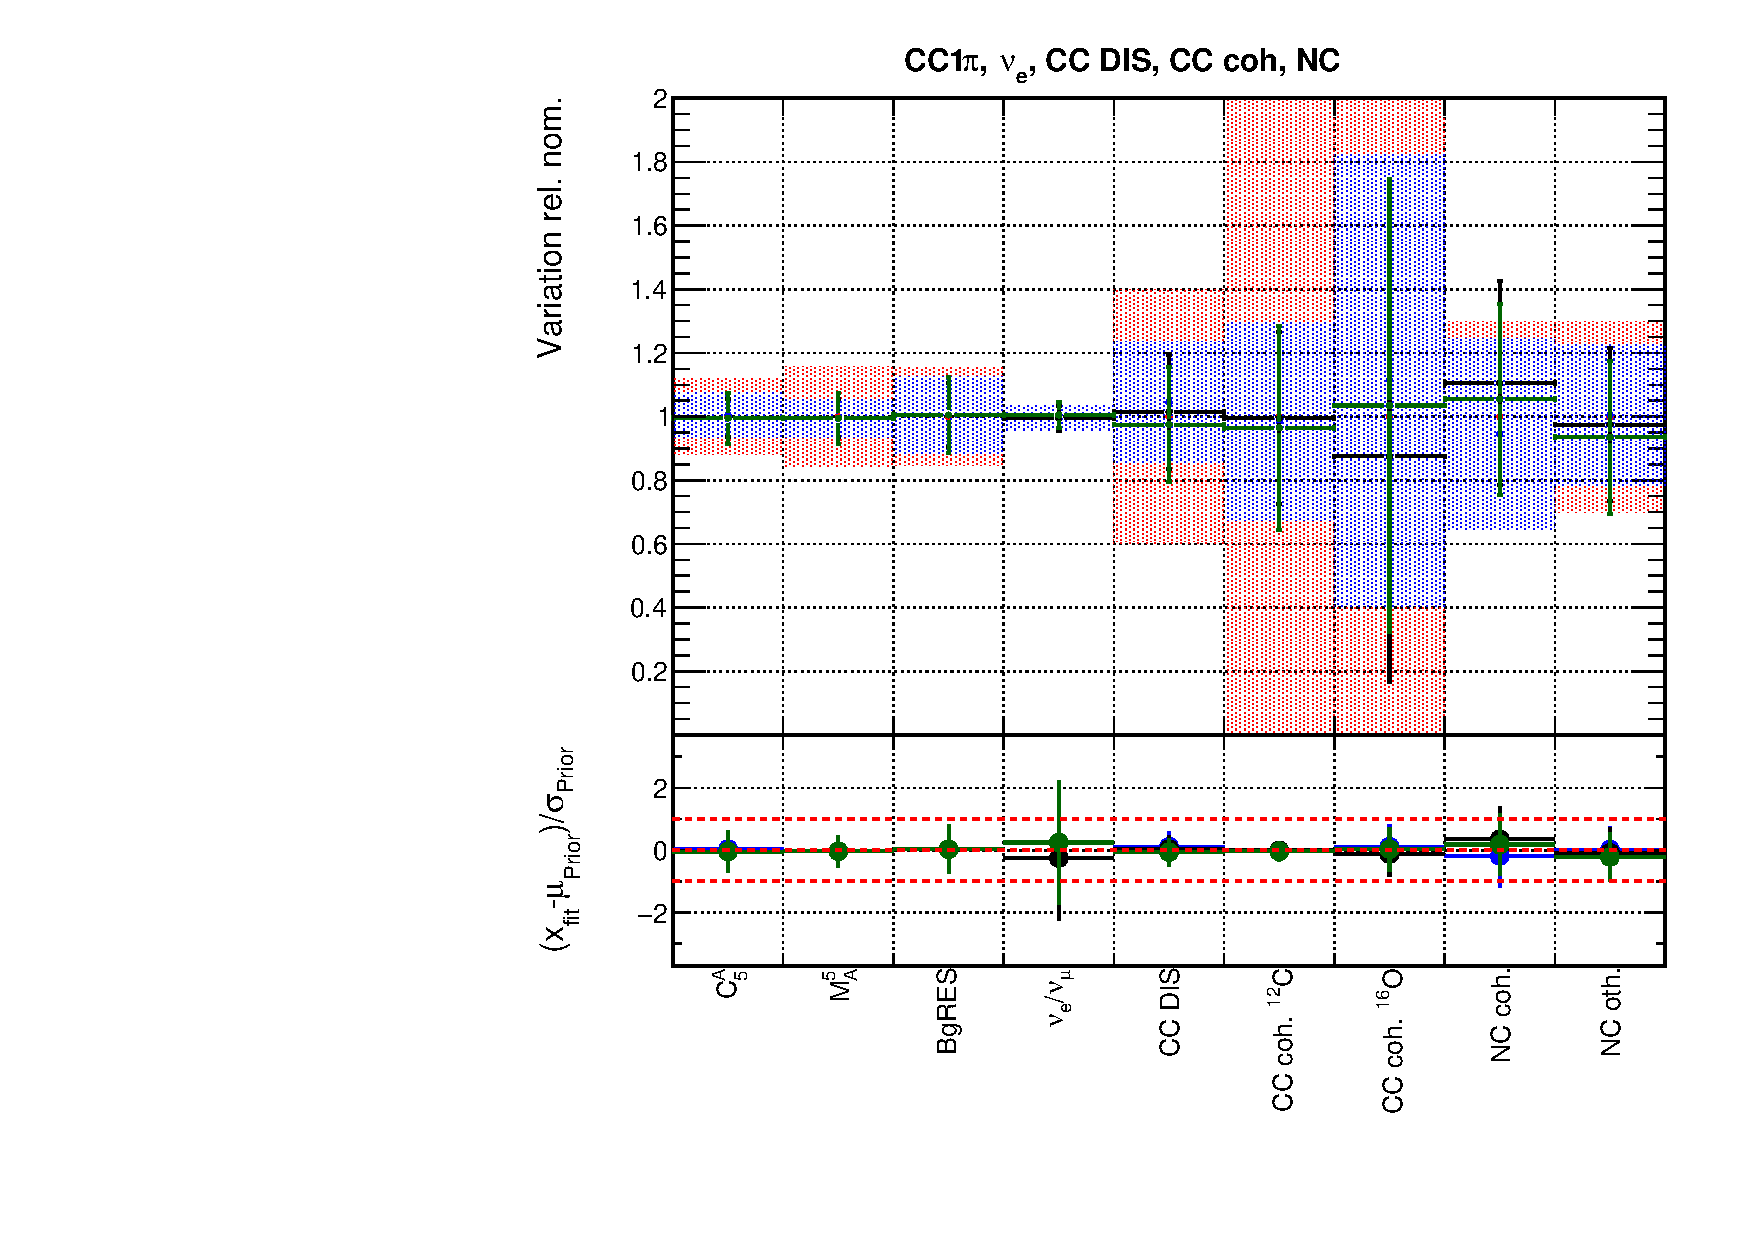
\includegraphics[width=0.95\linewidth]{figs/hptpcfitsxsec_2}
  \caption{CC1$\pi$, $\nu_e$, CC DIS, CC coh., NC}
\end{subfigure}
\begin{subfigure}{0.49\textwidth}
  \centering
  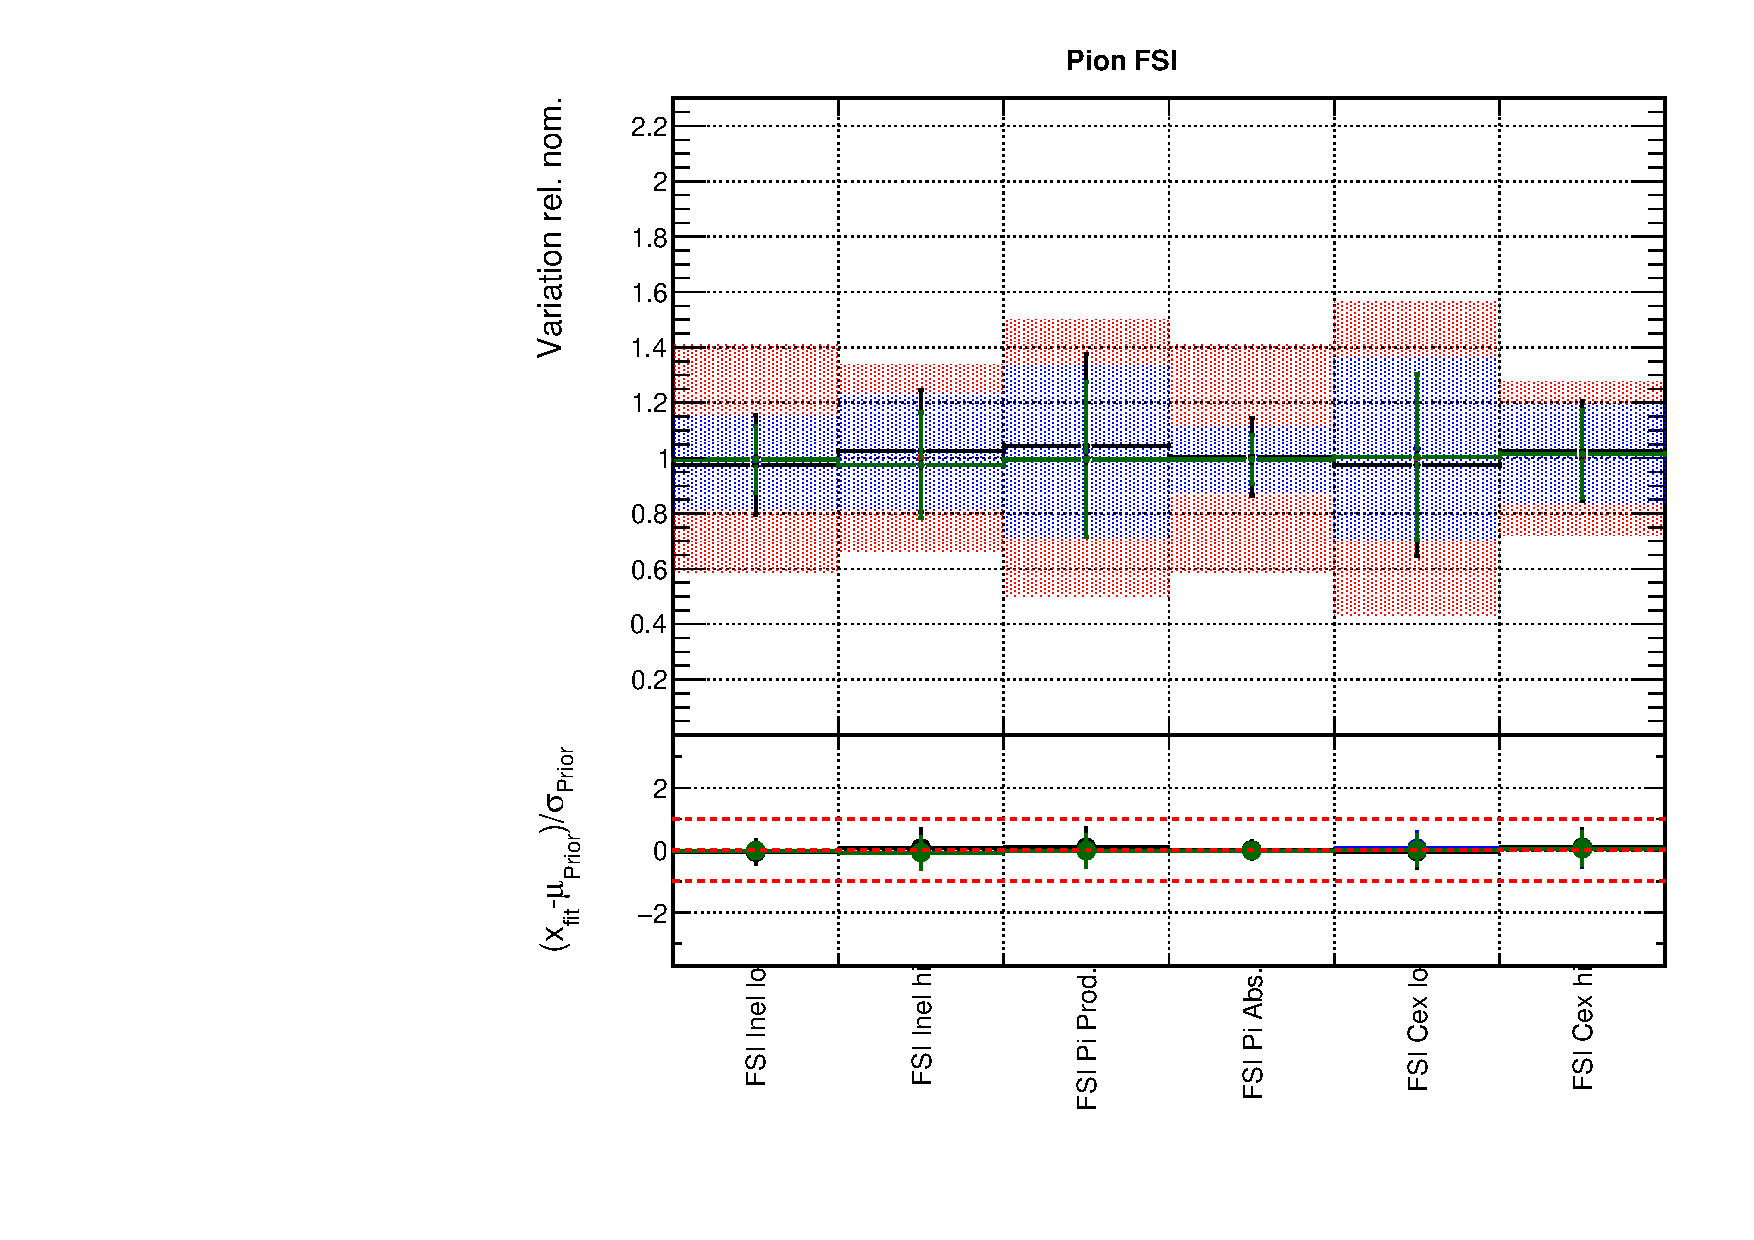
\includegraphics[width=0.95\linewidth]{figs/hptpcfitsxsec_3}
  \caption{FSI}
\end{subfigure}
\caption{Interaction parameters for ND280 $p_{\mu}$-cos$\theta_{\mu}$, HPTPC $p_{\mu}$-cos$\theta_{\mu}$, and HPTPC mixed STV fits.}
\label{fig:hptpcxsec}
\end{figure}

As expected, the postfit values of all parameters are very close to their nominal values. The slight differences are due to marginalisation effects, which are larger than for the full analysis fits due to the lower statistics.

The majority of flux parameters have a smaller postfit uncertainty for the HPTPC than ND280. The increase in number of events from lowering the detection thresholds allows a slight increase in the constraint on these systematics.

There is also a further reduction in the majority of postfit flux uncertainties for fitting in STVs rather than just $p_{\mu}$-cos$\theta_{\mu}$. This is a smaller effect however, and is not consistent across all energies.

Several of the interaction parameters also have a general trend of the HPTPC seeing better constraint than ND280, and the STVs being a slight improvement on just the lepton variables.

The size of the $M_{A}^{QE}$, Fermi momentum $^{12}$C, and binding energy $^{12}$C uncertainties are very similar in the three fits. The MEC $^{12}$C uncertainty has a stronger constraint for the HPTPC, but only a small improvement from the STVs. The $^{16}$O parameters have very little constraint in any of the fits as only FGD1 MC is used. 

Of the 1 $\pi$ parameters, the $I_{1/2}$ non-resonant background is the only uncertainty to reduce for the HPTPC compared to ND280. The STVs do not improve the constraint any further. The CC DIS and CC coh. $^{12}$C parameters have small improvements in constraint for HPTPC, but this is not reduced any further by the STVs. The CC coh. $^{16}$O has a similar postfit uncertainty for all three fits, as the constraint comes entirely from the prior. The NC parameters have similar postfit uncertainties for each of the fits.

The FSI parameters all have similar constraints for the HPTPC and ND280, but a significant improvement from using the STVs.

Overall, the majority of parameters have a smaller uncertainty for the HPTPC STV fit than the ND280 $p_{\mu}$-cos$\theta_{\mu}$ fit.

These results show that lowering detection thresholds, and using more kinematic information than just the lepton variables, can improve the constraint of systematic uncertainties in the fit. However, this is not a complete study, for a number of reasons. Firstly, without detector systematics in the fit the results are not entirely valid. These could correlate with the other parameters differently for the two detectors, altering the uncertainties in each fit.

There is also a low sample size used in this study compared to the full T2K oscillation analysis. Using the entire runs 2-9 MC to produce HPTPC-like events would give a better comparison of the potential sensitivities.

Furthermore, the HPTPC events are truth-smeared ND280 FGD1 events, and so the target is carbon. Future studies aiming for a more complete comparison of the sensitivity of the detectors should use a full simulation of an HPTPC with different target gasses. The target volume of an HPTPC would also be larger than that of ND280, increasing the target mass and therefore the number of interactions, which is not accounted for in this study. 

Further improvements to the fitting framework could also help achieve the full potential of an HPTPC. With the increase in statistics future experiments will benefit from, events could be binned in more than two kinematic variables. This would allow better characterisation of interactions, and so systematics could be applied to the target events more accurately. The systematics themselves could also be generated to be more appropriate for use with transverse kinematics. The systematics used in this study were designed to depend on the leptonic information in the event. As the lower detection thresholds allow better measurements of the hadronic side of interactions, models constructed to use this information would better use the full constraining power of an HPTPC.

However, this study does show that just by lowering detection thresholds and using different kinematic variables, systematic uncertainties gain a significant improvement in constraint compared to ND280. This is not just due to the increase in interactions, but because the extra interactions detected are at low momentum. By reducing cross-section systematics, different interaction model components can be distinguished, and in particular by probing the low momentum regions an HPTPC will allow nuclear FSI model tensions to be resolved. This will be crucial for reducing systematic uncertainties sufficiently to measure $\delta_{CP}$ to 5$\sigma$ in future long baseline neutrino oscillation experiments. The full constraining power of an HPTPC will be further improved on these results by the larger target mass and fitting in more than two kinematic variables. Doing a full scale simulation of the detector would give a better indication of the HPTPC's potential sensitivity.

\section{Summary}

This chapter has presented an overview of sensitivity studies for a proposed near detector for future long baseline neutrino oscillation experiments. For the next generation of experiments to achieve their target sensitivity, systematic uncertainties will need to be reduced to the 1-2$\%$ level. This will require tensions in nuclear models to be resolved.

Using a gas target will allow an HPTPC to probe the low momentum region of parameter space where nuclear models currently diverge. Increasing the pressure of the gas, combined with future Mega-Watt beams, means there can be enough detected events using a gaseous target. 

The 4-$\pi$ angular coverage and lower momentum thresholds of an HPTPC allow accurate measurement of the momentum and multiplicity of secondary particles. This allows STVs to be used to better characterise events affected by FSI, and so nuclear model tensions can be better resolved.

HPTPC MC events were produced by smearing the true kinematics of ND280 FGD1 MC events and using estimated improvements in detection thresholds. Asimov fits show an improvement in sensitivity from the estimated thresholds for an HPTPC compared to ND280, and for using a combination of different STVs for different samples compared to using lepton kinematics only.

Although a larger dataset, and full HPTPC simulation should be used for more comprehensive sensitivity studies, these results show that lowering detection thresholds and using different kinematic variables significantly improve the constraint on systematic uncertainties compared to ND280. This will allow nuclear models to be better distinguished in future long baseline neutrino oscillation experiments, which will be crucial for measuring $\delta_{CP}$ to 5$\sigma$.



\newpage